% !TeX root = constructions.tex

%%%%%%%%%%%%%%%%%%%%%%%%%%%%%%%%%%%%%%%%%%%%%%%%%%%%%%%%%%%%%%%%

\documentclass[11pt,a4paper]{report}

\usepackage{mathpazo}
\usepackage{microtype}
\usepackage{graphicx}
\usepackage{verbatim}
\usepackage{url}
\usepackage{bm}
\usepackage{float}
\usepackage{eqnarray}
\usepackage{titlesec}

\usepackage{tikz}
\usetikzlibrary{positioning,through,calc,intersections,arrows.meta,external}
\tikzexternalize[prefix=tikz/]
\tikzset{>=stealth} % Use stealth arrows

\textwidth=155mm
\textheight=235mm
\topmargin=0pt
\headheight=0pt
\oddsidemargin=5mm
\headsep=0pt
\parindent=0pt
\renewcommand{\baselinestretch}{1.1}
\setlength{\parskip}{0.3\baselineskip plus 1pt minus 1pt}
\addtolength{\jot}{3pt}

\newcommand*{\p}[1]{\textsf{\small #1}}
\newcommand*{\sm}[1]{$\scriptstyle #1$}
\newcommand*{\bover}[1]{\bm{\overline{#1}}}
\newcommand*{\erh}[1]{\setlength{\extrarowheight}{#1}}
\newcommand*{\disfrac}[2]{\displaystyle\frac{#1}{#2}}

\newenvironment{form}[1]{%
\begin{displaymath}%
\renewcommand{\arraystretch}{#1}%
\begin{array}{lcl}}%
{\end{array}%
\end{displaymath}%
}

%  Less space above chapter title
\makeatletter
\def\@makechapterhead#1{%
  {\parindent \z@ \raggedright \normalfont
    \ifnum \c@secnumdepth >\m@ne
        \centering\Large\bfseries \@chapapp\space \thechapter\par
        \hspace{.3em}
    \fi
    \Large \bfseries #1\par\nobreak
    \vskip 20\p@
  }}
\makeatother

\setcounter{tocdepth}{1}

%\includeonly{}

\begin{document}

\tikzsetfigurename{front}
% !TeX root = constructions.tex

\thispagestyle{empty}

\begin{center}
\textbf{\LARGE Surprising Geometric Constructions}

\bigskip
\bigskip
\bigskip
\bigskip

\textbf{\Large Moti Ben-Ari}

\bigskip
\bigskip

\url{http://www.weizmann.ac.il/sci-tea/benari/}
\end{center}
\vfill

\begin{footnotesize}
\begin{center}
\copyright{}\ 2019--20 by Moti Ben-Ari.
\end{center}

This work is licensed under the Creative Commons Attribution-NonCommercial-ShareAlike 3.0 Unported License. To view a copy of this license, visit \url{http://creativecommons.org/licenses/by-nc-sa/3.0/} or send a letter to Creative Commons, 444 Castro Street, Suite 900, Mountain View, California, 94041, USA.
\end{footnotesize}

\bigskip

\begin{center}

\includegraphics[width=.15\textwidth]{by-nc-sa.png}
\end{center}

\newpage
\thispagestyle{empty}
\mbox{}
\newpage
\thispagestyle{empty}

\tableofcontents
\newpage
\mbox{}
\newpage


\chapter{Introduction}

Geometric constructions are fundamental to Euclidean geometry and appear in secondary-school textbooks \cite{geometry}. Most students of mathematics will also know that three constructions are impossible: trisecting angle, squaring a circle and doubling a cube. There are many interesting and surprising geometrical constructions that are probably unknown to students and teachers. This document presents these constructions in great detail using only secondary-school mathematics.

The \LaTeX{} source can be found at \url{https://github.com/motib/constructions}.

Part~\ref{p.sec} presents constructions with the familiar straightedge and compass, as well as constructions known to the Greeks that use extensions of the straightedge and compass. In recent years, the art of origami---paper folding---has been given a mathematical formalization as described in Part~\ref{p.origami}. It may come as a surprise that constructions with origami are more powerful than constructions with straightedge and compass.

\section{Constructions with straightedge and compass}

\begin{description}
\item[Chapeter \ref{c.collapse}, the collapsing compass] The modern compass is a \emph{fixed compass} that maintains the distance between its legs when lifted off the paper. It can be used to construct a line segment of the same length as a given segment. The compass used in the ancient world was a \emph{collapsing compass} that does not maintain the distance between its legs when lifted from the paper. Euclid showed that any construction that can be done with a fixed compass can be done with a collapsing compass. Numerous incorrect proofs have been given based on incorrect diagrams \cite{toussaint}. In order to emphasize that a proof must not depend on a diagram, I ``prove'' that \emph{every} triangle is isoceles.

\item[Chapter \ref{c.trisect}, trisecting an angle] Trisecting an arbitrary angle is impossible, but the Greeks knew that any angle can be trisected using extensions of the straightedge and compass. This chapter presents constructions that trisect an angle using a neusis and a quadratrix. The quadratrix can also be used to square a circle.

\item[Chapter \ref{c.squaring}, squaring a circle] To square a circle requires the construction of a line segment of length $\pi$. This chapter presents three constructions of approximations to $\pi$, one by Adam Kochansky and two by Ramanujan.

\item[Chapter \ref{c.compass-only}, construction with only a compass] Are both a straightedge and a compass necessary? Lorenzo Mascheroni and Georg Mohr showed that a compass only is sufficient. 

\item[Chapter \ref{c.straightedge} ,construction with only a straightedge] Is a straightedge sufficient? The answer is no because a straightedge can ``compute'' only linear functions, whereas a compass can ``compute'' quadratic functions. Jacob Steiner proved that a straightedge is sufficient provided that somewhere in the plane a single circle exists. 
\end{description}

\section{Constructions with origami}

\begin{description}
\item[Chapter~\ref{c.axioms}, the axioms of origami] The seven axioms of origami can be formalized in mathematics. This chapters derives formulas for the axioms, together with numerical examples.

\item[Chapter~\ref{c.trisection}, trisecting an angle] Two methods for trisecting an angle with origami are given.

\item[Chapter~\ref{c.cube}, doubling a cube] Two methods for doubling a cube with origami are given.

\item[Chapter~\ref{c.lill}, finding roots] This chapter explains Eduard Lill's geometric method for finding real roots of any polynomial (actually, verifying that a value is a root). We demonstrate the method for cubic polynomials.

\item[Chapter~\ref{c.beloch}, constructing a cube root] Margharita P. Beloch published an implementation of Lill's method that can find a root of a cubic polynomial with one fold.

\end{description}


\tikzsetfigurename{collapse}
% !TeX root = constructions.tex

\part{Straightedge and Compass}\label{p.sec}


\chapter{Help, My Compass Collapsed!}\label{c.collapse}

\section{Fixed compasses and collapsing compasses}

In a modern compass used for geometric constructions the distance between the two legs can be fixed so that it is possible to copy a line segment or a circle from one position to another. We will call such a compass a \emph{fixed compass}. I have seen geometry textbooks that present the  construction a perpendicular bisector to a line segment as follows: construct two circles centered at the ends of the line segment such that the radii are equal and \emph{greater than half the length of the segment} (left diagram):

\vspace{-2ex}

\begin{center}
\begin{tikzpicture}[scale=0.5]
\begin{scope}
\coordinate (A) at (0,0);
\coordinate (B) at (4,0);
\draw (A) node[below left] {$A$} -- (B) node[below right] {$B$};
\fill (A) circle[radius=3pt];
\fill (B) circle[radius=3pt];
\draw[name path=larc] (A) ++(-60:3cm) arc (-60:60:3cm);
\draw[name path=rarc] (B) ++(-120:3cm) arc (-120:-240:3cm);
\path [name intersections={of=larc and rarc,by={b,t}}];
\fill (t) node[above right,xshift=-2pt,yshift=5pt] {$C$} circle[radius=3pt];
\fill (b) node[below left,xshift=2pt,yshift=-5pt] {$D$} circle[radius=3pt];
\draw ($ (b) ! 1.2 ! (t)$) -- ($ (t) ! 1.2 ! (b)$);
\end{scope}
\begin{scope}[xshift=12cm]
\coordinate (A) at (0,0);
\coordinate (B) at (4,0);
\draw (A) node[below left] {$A$} -- (B) node[below right] {$B$};
\fill (A) circle[radius=3pt];
\fill (B) circle[radius=3pt];
\draw[name path=larc] (A) ++(-80:4cm) arc (-80:80:4cm);
\draw[name path=rarc] (B) ++(-100:4cm) arc (-100:-260:4cm);
\path [name intersections={of=larc and rarc,by={b,t}}];
\fill (t) node[above right,xshift=-2pt,yshift=3pt] {$C$} circle[radius=3pt];
\fill (b) node[below left,xshift=2pt,yshift=-3pt] {$D$}circle[radius=3pt];
\draw ($ (b) ! 1.2 ! (t)$) -- ($ (t) ! 1.2 ! (b)$);
\end{scope}
\end{tikzpicture}
\end{center}

\vspace{-2ex}

Euclid used a \emph{collapsing compass} whose legs fold up when the compass is lifted off the paper. Teachers often use a collapsing compass consisting of a piece of chalk tied to a string. It is impossible to maintain a fixed radius when the chalk is removed from the blackboard. The right diagram above shows how to construct a perpendicular bisector with a collapsing compass: the length of the segment $AB$ is, of course, equal to the length of the segment $BA$, so the radii of the two circles are equal.

The proof that the line constructed is the perpendicular bisector is not at all elementary because relatively advanced concepts like congruent triangles have to be used. However, the proof that the same construction results in an equilateral triangle is very simple (right diagram below). The length of $AC$ equals the length of $AB$ since they are radii of the same circle, and for the same reason the length of $BC$ is equal to the length of $BA$. We have:
\[
AC=AB=BA=BC\,.
\]

\begin{center}
\begin{tikzpicture}[scale=0.5]
\begin{scope}
\coordinate (A) at (0,0);
\coordinate (B) at (4,0);
\draw (A) node[below left] {$A$} -- (B) node[below right] {$B$};
\fill (A) circle[radius=3pt];
\fill (B) circle[radius=3pt];
\draw[name path=larc] (A) ++(-60:3cm) arc (-60:60:3cm);
\draw[name path=rarc] (B) ++(-120:3cm) arc (-120:-240:3cm);
\path [name intersections={of=larc and rarc,by={b,t}}];
\fill (t) node[above right,xshift=-2pt,yshift=5pt] {$C$} circle[radius=3pt];
\fill (b) node[below left,xshift=2pt,yshift=-5pt] {$D$} circle[radius=3pt];
\draw (A) -- (t);
\draw (B) -- (t);
\end{scope}
\begin{scope}[xshift=12cm]
\coordinate (A) at (0,0);
\coordinate (B) at (4,0);
\draw (A) node[below left] {$A$} -- (B) node[below right] {$B$};
\fill (A) circle[radius=3pt];
\fill (B) circle[radius=3pt];
\draw[name path=larc] (A) ++(-80:4cm) arc (-80:80:4cm);
\draw[name path=rarc] (B) ++(-100:4cm) arc (-100:-260:4cm);
\path [name intersections={of=larc and rarc,by={b,t}}];
\fill (t) node[above right,xshift=-2pt,yshift=3pt] {$C$} circle[radius=3pt];
\fill (b) node[below left,xshift=2pt,yshift=-3pt] {$D$}circle[radius=3pt];
\draw (A) -- (t);
\draw (B) -- (t);
\end{scope}
\end{tikzpicture}
\end{center}

The left diagram above shows that for the construction with the fixed compass the triangle will be isosceles, but not necessarily equilateral.

This construction of an equilateral triangle is the first proposition in Euclid's \emph{Elements}. The second proposition shows how to copy a given line segment $AB$ to a segment of the same length, one of whose end points is a given point $C$. Therefore, a fixed compass adds no additional capability. Toussaint \cite{toussaint} showed that many incorrect constructions for this proposition have been given. In fact, it was Euclid who gave a correct construction! The following section presents Euclid's construction and the proof of its correctness. Then I show an incorrect construction that can be found even in modern textbooks.

\section{Euclid's construction for copying a line segment}

\textbf{Theorem:} Given a line segment $AB$ and a point $C$, a line segment can be constructed (using a collapsing compass) at $C$ whose length is equal to the length of $AB$:

\begin{center}
\begin{tikzpicture}[scale=0.4]
\begin{scope}
\coordinate (C) at (0,0);
\coordinate (A) at (2.5,0);
\coordinate (B) at (5.5,2);
\draw (A) node[below,xshift=-2pt,yshift=-2pt] {$A$} -- (B) node[right] {$B$};
\fill (A) circle[radius=3pt];
\fill (B) circle[radius=3pt];
\fill (C) node[below,xshift=2pt,yshift=-2pt] {$C$} circle[radius=3pt];
\end{scope}
\begin{scope}[xshift=12cm]
\coordinate (C) at (0,0);
\coordinate (A) at (2.5,0);
\coordinate (B) at (5.5,2);
\draw (A) node[below,xshift=-2pt,yshift=-2pt] {$A$} -- (B) node[right] {$B$};
\fill (A) circle[radius=3pt];
\fill (B) circle[radius=3pt];
\fill (C) node[below,xshift=2pt,yshift=-2pt] {$C$} circle[radius=3pt];
\draw (A) -- (C);
\path[name path=larc] (C) ++(-70:2.5cm) arc (-70:70:2.5cm);
\path[name path=rarc] (A) ++(-110:2.5cm) arc (-110:-250:2.5cm);
\path [name intersections={of=larc and rarc,by={d,D}}];
\fill (D) node[above] {$D$} circle[radius=3pt];
\draw (A) -- (D);
\draw (C) -- (D);
\end{scope}
\end{tikzpicture}
\end{center}

\textbf{Construction:}

Construct the line segment from $A$ to $C$.

Construct an equilateral triangle whose base is $AC$ (right diagram above). Label the third vertex $D$. By Euclid's first proposition, the triangle can be constructed using a collapsing compass.

Construct a ray that is a continuation of $DA$ and a ray that is a continuation of $DC$ (left diagram below).

Construct a circle centered at $A$ with radius $AB$. Label the intersection of the circle and the ray $DA$ by $E$ (right diagram below).

\begin{center}
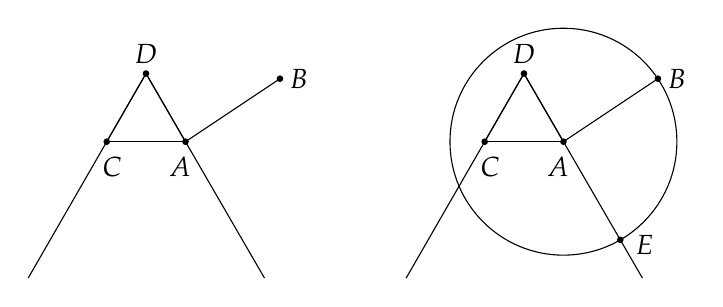
\begin{tikzpicture}[scale=0.4]
\begin{scope}
\coordinate (C) at (0,0);
\coordinate (A) at (2.5,0);
\coordinate (B) at (5.5,2);
\draw (A) node[below,xshift=-2pt,yshift=-2pt] {$A$} -- (B) node[right] {$B$};
\fill (A) circle[radius=3pt];
\fill (B) circle[radius=3pt];
\fill (C) node[below,xshift=2pt,yshift=-2pt] {$C$} circle[radius=3pt];
\draw (A) -- (C);
\path[name path=larc] (C) ++(-70:2.5cm) arc (-70:70:2.5cm);
\path[name path=rarc] (A) ++(-110:2.5cm) arc (-110:-250:2.5cm);
\path [name intersections={of=larc and rarc,by={d,D}}];
\fill (D) node[above] {$D$} circle[radius=3pt];
\draw (A) -- (D);
\draw (C) -- (D);
\draw[name path=ray2] (D) -- ($ (D) ! 3 ! (C) $);
\draw[name path=ray1] (D) -- ($ (D) ! 3 ! (A) $);
\end{scope}
\begin{scope}[xshift=12cm]
\coordinate (C) at (0,0);
\coordinate (A) at (2.5,0);
\coordinate (B) at (5.5,2);
\draw (A) node[below,xshift=-2pt,yshift=-2pt] {$A$} -- (B) node[right] {$B$};
\fill (A) circle[radius=3pt];
\fill (B) circle[radius=3pt];
\fill (C) node[below,xshift=2pt,yshift=-2pt] {$C$} circle[radius=3pt];
\draw (A) -- (C);
\path[name path=larc] (C) ++(-70:2.5cm) arc (-70:70:2.5cm);
\path[name path=rarc] (A) ++(-110:2.5cm) arc (-110:-250:2.5cm);
\path [name intersections={of=larc and rarc,by={d,D}}];
\fill (D) node[above] {$D$} circle[radius=3pt];
\draw (A) -- (D);
\draw (C) -- (D);
\draw[name path=ray2] (D) -- ($ (D) ! 3 ! (C) $);
\draw[name path=ray1] (D) -- ($ (D) ! 3 ! (A) $);
\node[draw,circle through=(B),name path=c1] at (A) {};
\path [name intersections={of=c1 and ray1,by={E,e}}];
\fill (E) node[right,xshift=2pt,yshift=-2pt] {$E$} circle[radius=3pt];
\end{scope}
\end{tikzpicture}
\end{center}

Construct a circle centered at $D$ with radius $DE$. Label the intersection of the circle and the ray $DC$ by $F$:

\begin{center}
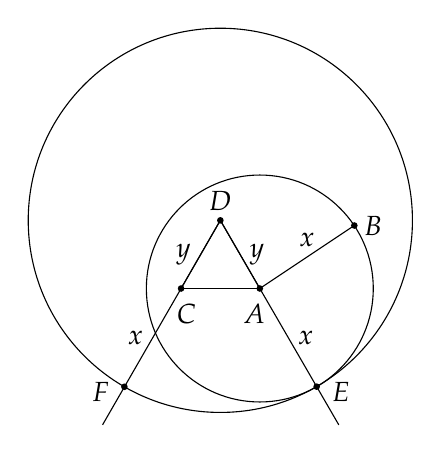
\begin{tikzpicture}[scale=0.4]
\coordinate (C) at (0,0);
\coordinate (A) at (2.5,0);
\coordinate (B) at (5.5,2);
\draw (A) node[below,xshift=-2pt,yshift=-2pt] {$A$} -- node[above] {$x$} (B) node[right] {$B$};
\fill (A) circle[radius=3pt];
\fill (B) circle[radius=3pt];
\fill (C) node[below,xshift=2pt,yshift=-2pt] {$C$} circle[radius=3pt];
\draw (A) -- (C);
\path[name path=larc] (C) ++(-70:2.5cm) arc (-70:70:2.5cm);
\path[name path=rarc] (A) ++(-110:2.5cm) arc (-110:-250:2.5cm);
\path [name intersections={of=larc and rarc,by={d,D}}];
\fill (D) node[above] {$D$} circle[radius=3pt];
\draw (A) -- node[right] {$y$} (D);
\draw (C) -- node[left] {$y$} (D);
\draw[name path=ray2] (D) -- ($ (D) ! 3 ! (C) $);
\draw[name path=ray1] (D) -- ($ (D) ! 3 ! (A) $);
\node[draw,circle through=(B),name path=c1] at (A) {};
\path [name intersections={of=c1 and ray1,by={E,e}}];
\fill (E) node[right,xshift=2pt,yshift=-2pt] {$E$} circle[radius=3pt];
\node[draw,circle through=(E),name path=c2] at (D) {};
\path [name intersections={of=c2 and ray2,by={F,f}}];
\fill (F) node[left,xshift=-2pt,yshift=-2pt] {$F$} circle[radius=3pt];
\path (A) -- node[right] {$x$} (E);
\path (C) -- node[left] {$x$} (F);
\end{tikzpicture}
\end{center}

\textbf{Claim:} The length of the line segment $CF$ is equal to the length of $AB$.

\textbf{Proof:} $DC=DA$ because $\triangle ACD$ is equilateral. $AE=AB$ because they are radii of the same circle centered at $A$. $DF=DE$ because they are radii of the same circle centered at $D$. Therefore, the length of the line segment $CF$ is:
\[
CF=DF-DC=DE-DC=DE-DA=AE=AB\,.
\]


%%%%%%%%%%%%%%%%%%%%%%%%%%%%%%%%%%%%%%%%%%%%%%%%%%%%%%%%%%%%%%%

\section{An incorrect construction for copying a line segment}\label{s.erroneous}

\textbf{Construction(\cite{rusty}):}

Construct a circle centered at $A$ with radius $AB$:

\begin{center}
\begin{tikzpicture}[scale=0.4]
\begin{scope}
\coordinate (C) at (-2,0);
\coordinate (A) at (2.5,0);
\coordinate (B) at (4.5,1.5);
\draw (A) node[below,xshift=-2pt,yshift=-2pt] {$A$} -- (B) node[right] {$B$};
\fill (A) circle[radius=3pt];
\fill (B) circle[radius=3pt];
\fill (C) node[below,xshift=2pt,yshift=-2pt] {$C$} circle[radius=3pt];
\end{scope}
\begin{scope}[xshift=12cm]
\coordinate (C) at (-2,0);
\coordinate (A) at (2.5,0);
\coordinate (B) at (4.5,1.5);
\draw (A) node[below,xshift=-2pt,yshift=-2pt] {$A$} -- (B) node[right] {$B$};
\fill (A) circle[radius=3pt];
\fill (B) circle[radius=3pt];
\fill (C) node[below,xshift=2pt,yshift=-2pt] {$C$} circle[radius=3pt];
\node[draw,circle through=(B),name path=c1] at (A) {};
\end{scope}
\end{tikzpicture}
\end{center}

Construct a circle centered at $A$ with radius $AC$ and a circle centered at $C$ with radius $AC=CA$. Label the intersections of the two circles $E,F$. Label the intersection of the circle centered at $C$ and the circle centered at $A$ with radius $AB$ by $D$:

\begin{center}
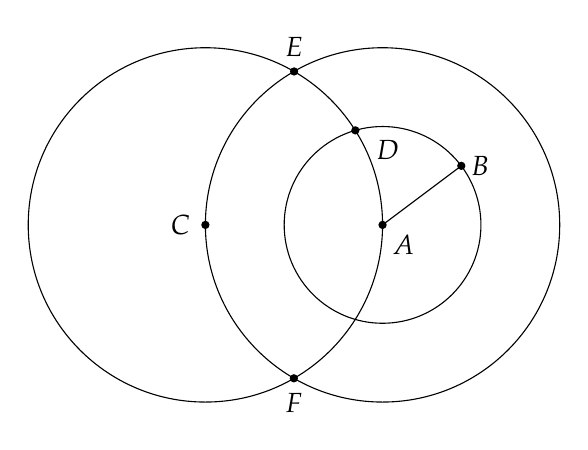
\begin{tikzpicture}[scale=0.5]
\coordinate (C) at (-2,0);
\coordinate (A) at (2.5,0);
\coordinate (B) at (4.5,1.5);
\draw (A) node[below right] {$A$} -- (B) node[right] {$B$};
\fill (A) circle[radius=3pt];
\fill (B) circle[radius=3pt];
\fill (C) node[left,xshift=-2pt] {$C$} circle[radius=3pt];
\node[draw,circle through=(B),name path=c1] at (A) {};
\node[draw,circle through=(C),name path=c2] at (A) {};
\node[draw,circle through=(A),name path=c3] at (C) {};
\path [name intersections={of=c1 and c3,by={D,f}}];
\path [name intersections={of=c2 and c3,by={E,F}}];
\fill (D) node[below right,xshift=4pt] {$D$} circle[radius=3pt];
\fill (E) node[above,yshift=2pt] {$E$} circle[radius=3pt];
\fill (F) node[below,yshift=-2pt] {$F$} circle[radius=3pt];
\end{tikzpicture}
\end{center}

Construct a circle centered at $E$ with radius $ED$. Label the intersection of this circle with the circle centered at $A$ with radius $AC$ by $G$:

\begin{center}
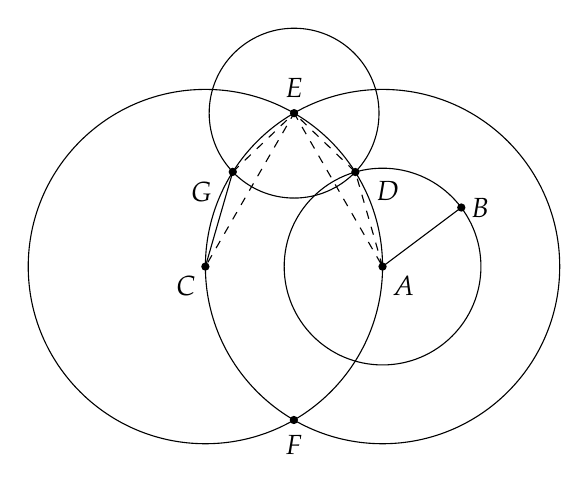
\begin{tikzpicture}[scale=0.5]
\coordinate (C) at (-2,0);
\coordinate (A) at (2.5,0);
\coordinate (B) at (4.5,1.5);
\draw (A) node[below right] {$A$} -- (B) node[right] {$B$};
\fill (A) circle[radius=3pt];
\fill (B) circle[radius=3pt];
\fill (C) node[below left] {$C$} circle[radius=3pt];
\node[draw,circle through=(B),name path=c1] at (A) {};
\node[draw,circle through=(C),name path=c2] at (A) {};
\node[draw,circle through=(A),name path=c3] at (C) {};
\path [name intersections={of=c1 and c3,by={D,f}}];
\path [name intersections={of=c2 and c3,by={E,F}}];
\fill (D) node[below right,xshift=4pt] {$D$} circle[radius=3pt];
\fill (E) node[above,yshift=2pt] {$E$} circle[radius=3pt];
\fill (F) node[below,yshift=-2pt] {$F$} circle[radius=3pt];
\node[draw,circle through=(D),name path=c4] at (E) {};
\path [name intersections={of=c2 and c4,by={g,G}}];
\fill (G) node[below left,xshift=-4pt] {$G$} circle[radius=3pt];
\draw (C) -- (G);
\draw[dashed] (G) -- (E) -- (C);
\draw[dashed] (A) -- (D) -- (E) -- cycle;
\end{tikzpicture}
\end{center}

\textbf{Claim:} The length of the line segment $GC$ is equal to the length of $AB$.

\textbf{Proof:} We shall show that $\triangle ADE\cong\triangle CGE$. If so, $CG=AD=AB$ because $AB,AD$ are radii of the smaller circle centered at $A$. The circle centered at $C$ has the same radius as the circle centered at $A$ that goes through $E$, so we can consider that they are the ``same'' circle.

$EG=ED$ because they are radii of the circle centered at $E$ and $EC=EA$ because they are radii of the ``same'' circle. $\angle GCE=\angle DAE$ because they are central angles that intercept the ``same'' chord and $\angle CGE=\angle ADE$ because they are inscribed angles intercepting the ``same'' chord. Therefore, $\angle GEC=\angle DEA$ and $\triangle GEC\cong \triangle DAE$ by SAS. 

The answer: there isn't any error in the proof! The problem arises from a different source: the equality $AB=GC$ holds only when the length of $AB$ is less that the length of $AC$. In contrast, Euclid's construction and proof are true, independent of the relative lengths of  $AB$ and $AC$, and of the position of the point $C$ relative to the line segment $AB$ (\cite{toussaint}).


%%%%%%%%%%%%%%%%%%%%%%%%%%%%%%%%%%%%%%%%%%%%%%%%%%%%%%%%%%%%%%%

\section{A ``simpler'' construction for copying a line segment}

Given a line segment $AB$ and a point $C$, if we can build a parallelogram with these three points as its vertices, we obtain a line segment with $C$ at one end whose length is equal to the length of $AB$ (left diagram left):
\begin{center}
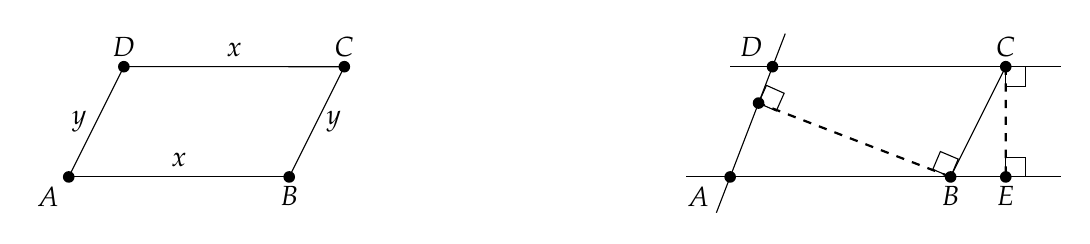
\begin{tikzpicture}[scale=0.7]
\coordinate (A) at (0,0);
\coordinate (B) at (4,0);
\coordinate (C) at (5,2);
\draw (A) -- (B);
\path (A) -- node[above] {$x$} (B);
\fill (A) node[below left] {$A$} circle[radius=3pt];
\fill (B) node[below] {$B$} circle[radius=3pt];
\fill (C) node[above] {$C$} circle[radius=3pt];
\draw (B) -- node[right] {$y$} (C);
\coordinate (D) at ($(C)+(-40mm,0cm)$);
\draw (D) -- node[above] {$x$} (C);
\draw (A) -- node[left] {$y$} (D);
\fill (D) node[above] {$D$} circle[radius=3pt];
\begin{scope}[xshift=12cm]
\coordinate (A) at (0,0);
\coordinate (B) at (4,0);
\coordinate (C) at (5,2);
\draw ($ (B) ! 1.2 ! (A) $) -- ($ (A) ! 1.5 ! (B) $);
\path (A) -- (B);
\fill (A) node[below left,xshift=-4pt] {$A$} circle[radius=3pt];
\fill (B) node[below] {$B$} circle[radius=3pt];
\fill (C) node[above] {$C$} circle[radius=3pt];
\draw (B) -- (C);
\draw[name path=ray1] ($(C)+(-5cm,0cm)$) -- ($(C)+(1cm,0cm)$);
\draw[name path=ray2] ($(A)+(-.25,-.65)$) -- ($(A)+(1,2.6)$);
\path [name intersections={of=ray1 and ray2,by={D}}];
\fill (D) node[above left] {$D$} circle[radius=3pt];
\coordinate (E) at (C |- B);
\draw[thick,dashed] (C) -- (E);
\fill (E) node[below] {$E$} circle[radius=3pt];
\draw[rotate=-90] (C) rectangle +(10pt,10pt);
\draw (E) rectangle +(10pt,10pt);
\coordinate (F) at ($(A)!(B)!(D)$);
\fill (F) circle[radius=3pt];
\draw[thick,dashed] (B) -- (F);
\draw[rotate=-24] (F) rectangle +(10pt,10pt);
\draw[rotate=67] (B) rectangle +(10pt,10pt);
\end{scope}
\end{tikzpicture}
\end{center}
This construction can be found in \cite[pp. 207--208]{roads}.

\textbf{Construction (right diagram):}

Construct the line segment from $B$ to $C$.

Construct an altitude from $C$ to the line containing the line segment $AB$. Label the intersection by $D$.

Construct an altitude to the line segment $CD$ at $C$. This line is parallel to $AB$.

Use a similar method to construct a line parallel to $BC$ through $A$. Label the intersection of the two lines by $D$.

$AD\|BC$, $AB\|DC$ and by definition $ABCD$ is a parallelogram, so $AB=CD$ as required.

\textbf{Construction with a collapsing compass:} We will show that it is possible to construct an altitude through a given point with a collapsing compass. Construct a circle centered at $C$ with a radius that is greater than the distance of $C$ from the line. Label the intersections with the line by $D,E$. Construct circles centered at $D,E$ with radii $DC=EC$:
\begin{center}
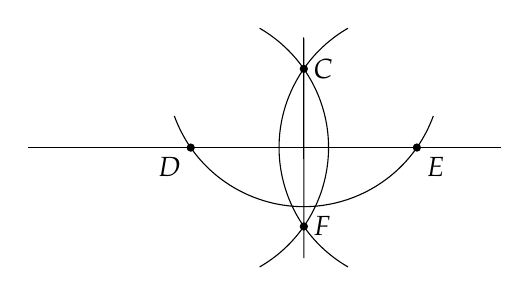
\begin{tikzpicture}[scale=0.5]
\coordinate (A) at (0,0);
\coordinate (B) at (4,0);
\coordinate (C) at (5,2);
\draw[name path=ray] ($ (B) ! 1.5 ! (A) $) -- ($ (A) ! 2.5 ! (B) $);
%\fill (A) node[below] {$A$} circle[radius=3pt];
%\fill (B) node[below] {$B$} circle[radius=3pt];
\fill (C) node[right] {$C$} circle[radius=3pt];
\draw[name path=arc] (C) ++(-160:3.5cm) arc (-160:-20:3.5cm);
\path [name intersections={of=arc and ray,by={D,E}}];
\fill (D) node[below left] {$D$} circle[radius=3pt];
\fill (E) node[below right] {$E$} circle[radius=3pt];
\draw[name path=larc] (D) ++(-60:3.5cm) arc (-60:60:3.5cm);
\draw[name path=rarc] (E) ++(-120:3.5cm) arc (-120:-240:3.5cm);
\path [name intersections={of=larc and rarc,by={b,t}}];
\fill (b) node[right] {$F$} circle[radius=3pt];
\draw ($ (b) ! 1.2 ! (t)$) -- ($ (t) ! 1.2 ! (b)$);
\end{tikzpicture}
\end{center}
The line connecting the intersections of the circles $C,F$ is an altitude through $C$.

The proof the correctness of this construction is much more difficult than Euclid's proof of his construction.

%%%%%%%%%%%%%%%%%%%%%%%%%%%%%%%%%%%%%%%%%%%%%%%%%%%%%%%%%%%%%%%

\section{Don't trust a diagram}

Section~\ref{s.erroneous} showed that a diagram can be misleading. We now prove that \emph{all} triangles are isosceles!
\begin{center}
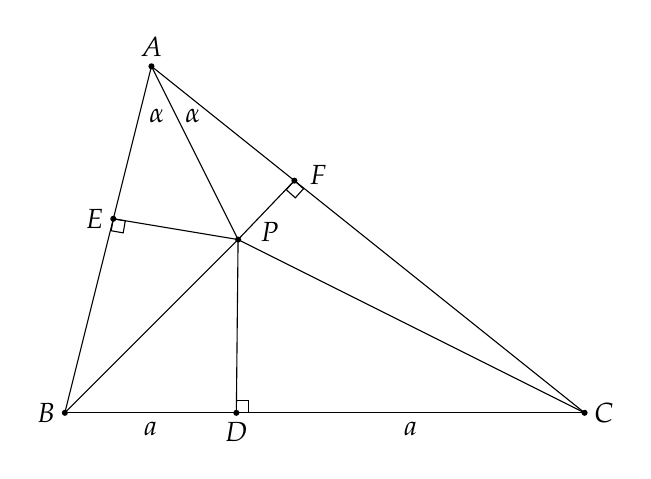
\begin{tikzpicture}[scale=1.1]
\coordinate (P) at (0,0);
\node[xshift=4mm,yshift=1mm] at (P) {$P$};
\coordinate [label=left:$B$] (B)  at (-2,-2);
\coordinate [label=right:$C$] (C)  at (4,-2);
\coordinate [label=above:$A$] (A)  at (-1,2);
\node[below,yshift=-12pt,xshift=2pt] at (A) {$\alpha$};
\node[below,yshift=-12pt,xshift=15pt] at (A) {$\alpha$};
\draw (A) -- (B);
\draw (A) -- (C);
\draw (B) -- (C);
\draw (A) -- (P);
\draw (B) -- (P);
\draw (C) -- (P);
\coordinate[label=left:$E$] (E) at ($ (A) ! .44 ! (B) $);
\draw[rotate=-100] (E) rectangle +(4pt,4pt);
\draw (P) -- (E);
\coordinate (F) at ($ (A) ! .33 ! (C) $);
\node[right,xshift=2pt,yshift=2pt] at (F) {$F$};
\draw[rotate=-132] (F) rectangle +(4pt,4pt);
\draw (P) -- (F);
\coordinate[label=below:$D$] (D) at ($ (B) ! .33 ! (C) $);
\draw (D) rectangle +(4pt,4pt);
\draw (P) -- (D);
\node[left] at ($ (A) ! .5 ! (E) $) {};
\node[left] at ($ (B) ! .5 ! (E) $) {};
\node[below] at ($ (B) ! .5 ! (D) $) {$a$};
\node[below] at ($ (C) ! .5 ! (D) $) {$a$};
\node[right,xshift=2pt] at ($ (A) ! .5 ! (F) $) {};
\node[right,xshift=2pt] at ($ (C) ! .5 ! (F) $) {};
\foreach \n in {A,B,C,D,E,F,P} {
  \fill (\n) circle[radius=1pt];
}
\end{tikzpicture}
\end{center}
Given an arbitrary triangle $\triangle ABC$, let $P$ be the intersection of the angle bisector of $\angle BAC$ and the perpendicular bisector $BC$. Label by $D,E,F$ the intersections of the altitudes from $P$ to the sides $BC, AB,AC$. $\triangle APF\cong \triangle APE$ because they are right triangles with equal angles $\alpha$ and a common side $AP$.

$\triangle DPC\cong \triangle DPB$ SAS because $PD$ is a common side, $\angle PDB=\angle PDC=90$ and $BD=DC=a$ because $PD$ is the perpendicular bisector of $BC$. $\triangle EPB\cong \triangle EPC$ because $EP=PF$ by the first congruence and $PB=PC$ by the second congruence. By combining the equations we get that $\triangle ABC$ is isoceles:
\[
AB= AE+EB=AF+FC =AC\,.
\]
The problem with the proof is that the diagram is incorrect because point $P$ is \emph{outside} the triangle, as can be seen from the following diagram constructed using GeoGebra:

\bigskip

\begin{center}
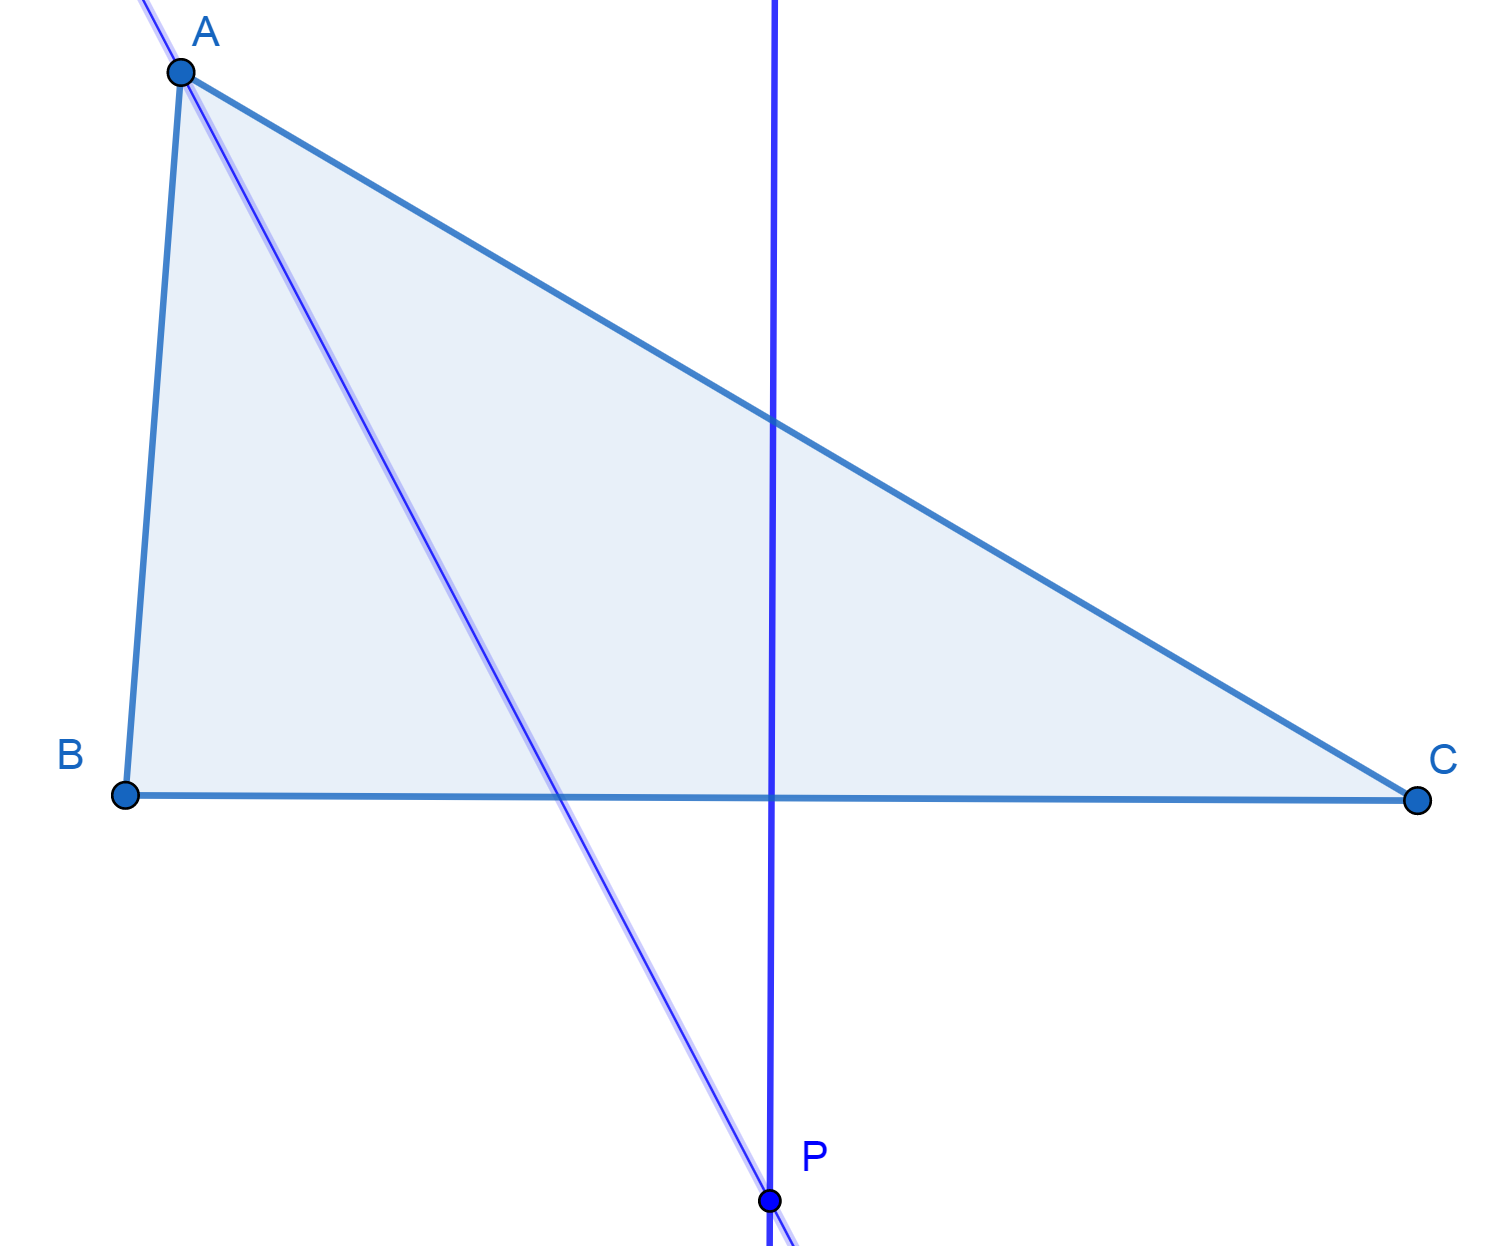
\includegraphics[width=.5\textwidth]{isoceles}
\end{center}



\tikzsetfigurename{trisect-an-angle}
% !TeX root = constructions.tex

\chapter{How to Trisect an Angle (With a Little Help from a Friend)}\label{c.trisect}

It is well known that it is impossible to trisect an arbitrary angle using a compass and a straightedge. The reason is that trisection requires the construction of cube roots, but the compass and straightedge can only construct lengths that are expressions built from the four arithmetic operators and square roots.

Greek mathematicians discovered that if other instruments are allowed, angles can be trisected \cite{wiki:tri}. Section~\ref{s.neusis} presents a construction of Archimedes using a simple instrument called a \emph{neusis} \cite{wiki:neu}. Section~\ref{s.q} shows a more complex construction of Hippias using the \emph{quadratrix} \cite{wiki:quad}. As a bonus, Section~\ref{s.square} shows that the quadratrix can square a circle.

%%%%%%%%%%%%%%%%%%%%%%%%%%%%%%%%%%%%%%%%%%%%%%%%%%%%%%%%%%%%%

\section{Trisection using the neusis}\label{s.neusis}

In geometry textbooks, constructions are performed using a ``straightedge'' and a compass. The term straightedge is used instead of ``ruler'' because a straightedge has no marks on it. The only operation it can perform is to construct a straight line between two points, while a ruler can measure distances. To trisect an angle all we need is a straightedge with two marks that are a fixed distance apart, called a \emph{neusis}. We define the distance between the marks as $1$:
\begin{center}
\begin{tikzpicture}[scale=3.5]
\draw (-1,1.05) rectangle +(3.2,.1);
\draw[thick] (1.89,1.05) -- +(0,.1);
\draw[thick] (.73,1.05) -- +(0,.1);
\draw[<->] (.73,1.25) -- node[fill=white] {$1$} (1.89,1.25);
\end{tikzpicture}
\end{center}

Let $\alpha$ be an arbitrary angle $\angle ABE$ within a circle with center $B$ and radius $1$. The circle can be constructed by setting the compass to the distance between the marks on the neusis. Extend the radius $EB$ beyond the circle. Place an edge of the neusis on $A$ and move it until it intersects the extension of $EB$ at $D$ and the circle at $C$, using the marks so that the length of the line segment $CD$ is $1$. Draw the line $AD$:

\begin{center}
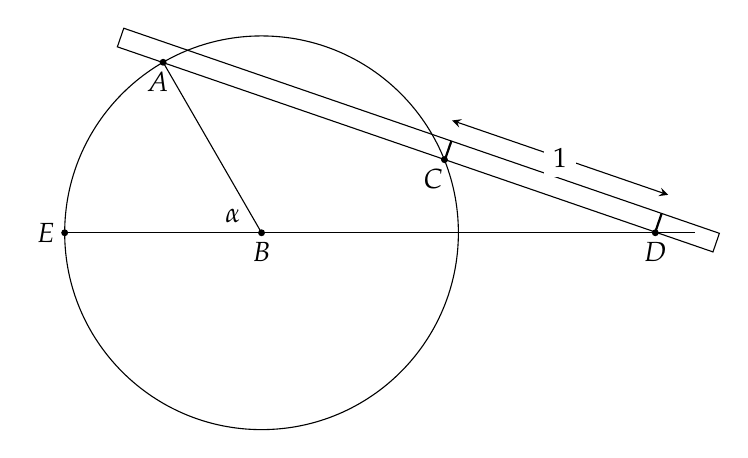
\begin{tikzpicture}[scale=2.5]
\coordinate (origin) at (0,0) node[below] {$B$} ;
\draw[name path=circle] (origin) circle [radius=1];
\draw (origin) node[above left,xshift=-4pt] {$\alpha$} -- (120:1) coordinate (a) node[below,xshift=-2pt] {$A$} ;
\draw (-1,0) -- (2.2,0);
\path[name path=ad] (a) -- (0,0 -| 2,0) coordinate (d) node[below] {$D$} ;
\path[name intersections={of=circle and ad,by={c,a1}}];
\fill (origin) circle [radius=.5pt];
\fill (a) circle [radius=.5pt];
\fill (c) circle [radius=.5pt] node [below,xshift=-4pt] {$C$};
\fill (d) circle [radius=.5pt];
\fill (-1,0) circle [radius=.5pt] node [left] {$E$};
\begin{scope}[rotate=-19,yshift=-11.25pt]
\draw (-1,1.05) rectangle +(3.2,.1);
\draw[thick] (1.89,1.05) -- +(0,.1);
\draw[thick] (.76,1.05) -- +(0,.1);
\draw[<->] (.73,1.25) -- node[fill=white] {$1$} (1.89,1.25);
\end{scope}
\end{tikzpicture}
\end{center}

\newpage

Draw line $BC$ and label the angles and line segments as shown:

\begin{center}
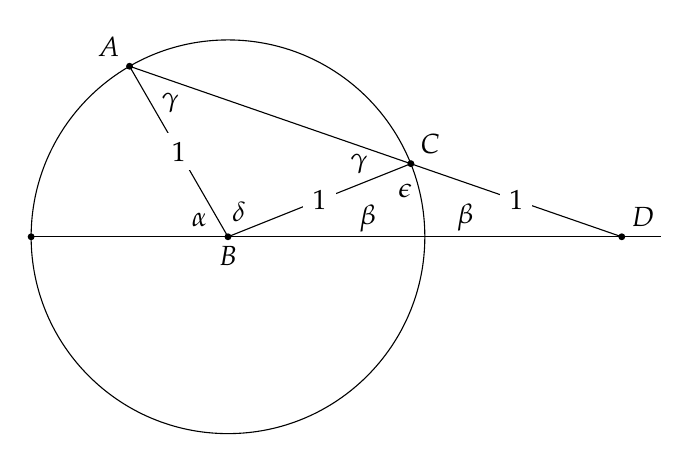
\begin{tikzpicture}[scale=2.5]
\coordinate (origin) at (0,0) node[below] {$B$} ;
\draw[name path=circle] (origin) circle [radius=1];
\draw (origin) node[above left,xshift=-4pt] {$\alpha$} node[above,xshift=4pt,yshift=2pt] {$\delta$} node[above right,xshift=44pt,yshift=-2pt] {$\beta$} -- node[fill=white] {$1$} (120:1) coordinate (a) node[above left] {$A$} ;
\draw (-1,0) -- (2.2,0);
\draw[name path=ad] (a) node[below right,xshift=8pt,yshift=-6pt] {$\gamma$} -- (0,0 -| 2,0) coordinate (d) node[left,xshift=-50pt,yshift=7pt] {$\beta$} node[above right] {$D$} ;
\path[name intersections={of=circle and ad,by={c,a1}}];
\draw (origin) -- node[fill=white] {$1$}(c) node[above right] {$C$} node[left,xshift=-12pt] {$\gamma$} node[below,xshift=-2pt,yshift=-4pt] {$\epsilon$};
\fill (origin) circle [radius=.5pt];
\fill (a) circle [radius=.5pt];
\fill (d) circle [radius=.5pt];
\fill (c) circle [radius=.5pt];
\fill (-1,0) circle [radius=.5pt];
\path (c) -- node[fill=white] {$1$} (d);
%\begin{scope}[rotate=-20]
%\draw (-1,1.05) rectangle +(3.2,.1);
%\draw[thick] (1.89,1.05) -- +(0,.1);
%\draw[thick] (.73,1.05) -- +(0,.1);
%\draw[<->] (.73,1.25) -- node[fill=white] {$1$} (1.89,1.25);
%\end{scope}
\end{tikzpicture}
\end{center}

Both $\triangle ABC$ and $\triangle BCD$ are isoceles: $AB=BC$ since both are radii and $BC=CD$ by construction using the neusis. A computation (using the facts that the angles of a triangle and supplemenary angles add up to $180$ radians) shows that $\beta$ trisects $\alpha$:
\erh{1pt}
\begin{equationarray*}{rcl}
\epsilon &=& \pi - 2\beta\\
\gamma &=& \pi - \epsilon = 2\beta\\
\delta &=& \pi - 2\gamma = \pi - 4\beta\\
\alpha &=& \pi - \delta - \beta\\
&=& 4\beta -\beta\\
&=& 3\beta\,.
\end{equationarray*}

\vspace{-2ex}

%%%%%%%%%%%%%%%%%%%%%%%%%%%%%%%%%%%%%%%%%%%%%%%%%%%%%%%%%%%%%

\section{Trisection using the quadratrix}\label{s.q}

The following diagram shows a \emph{quadratrix compass}: two (unmarked) straightedges connected by a joint that constrains them to move together. One straightedge moves parallel to the $x$-axis from $DC$ to $AB$, while the second straightedge is allowed to rotate around the origin at $A$ until it lies horizontally along $AB$. The curve traced by the joint of the two straightedges is called the \emph{quadratrix curve} or simply the \emph{quadratrix}.

\begin{center}
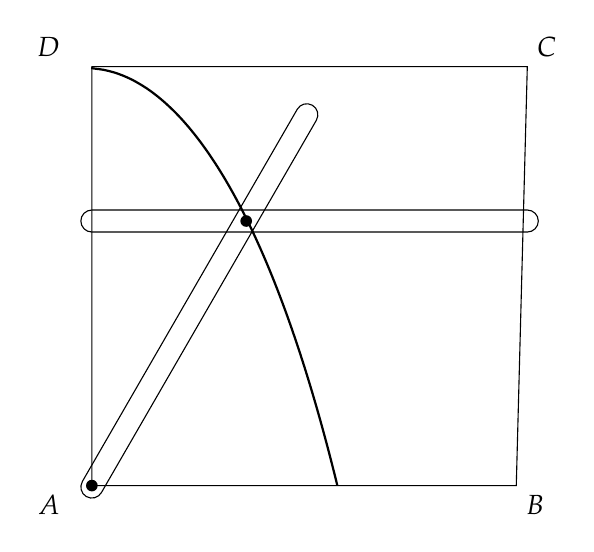
\begin{tikzpicture}[scale=.7,domain=.03:1.555,samples=100]
\draw (.1,.2) node[below left,xshift=-8pt] {$A$} -- (7.8,.2) node[below right] {$B$} -- (8,7.8) node[above right] {$C$} -- (.1,7.8) node[above left,xshift=-8pt] {$D$} -- cycle;
%\draw (.1,7.8) -- (.1,.2) -- (8,.1) -- (8,7.8);
\draw[rounded corners,rotate=60] (0,-.2) rectangle (8.2,.2);
\draw[rounded corners] (-.1,4.8) rectangle (8.2,5.2);
\fill (2.9,5) circle [radius=3pt];
\fill (.1,.2) circle [radius=3pt];
\draw[thick] plot (4.6*.637*\x,{12.2*.637*\x*cot(\x r)});
\end{tikzpicture}
\end{center}

\vspace{-2ex}

As the horizontal straightedge is moved down at a constant velocity, the other straightedge is constrained to move at a constant angular velocity. In fact, that is the definition of the quadratrix curve. As the $y$-coordinate of the horizontal straightedge decreases from $1$ to $0$, the angle of the other straightedge relative to the $x$-axis decreases from $90^\circ$ to $0^\circ$. The following diagram shows how this can be used to trisect an arbitrary angle $\alpha$:

\vspace{-2ex}

\begin{center}
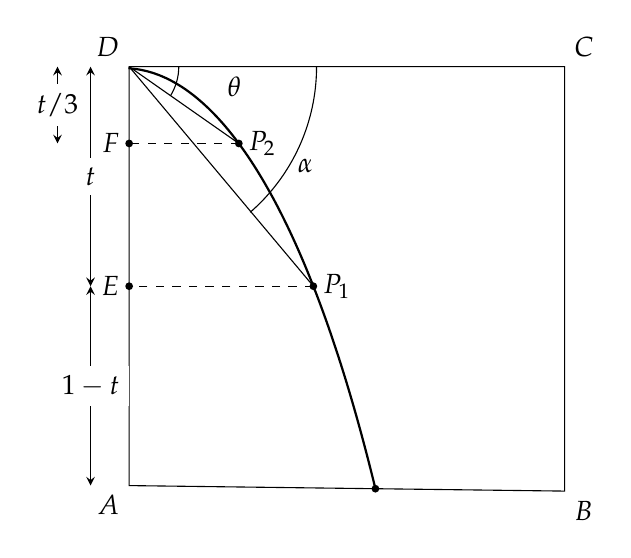
\begin{tikzpicture}[scale=.7,domain=.03:1.562,samples=100]
\draw (.1,7.8) coordinate (start) node[above left] {$D$} node[below right,xshift=32pt] {$\theta$} -- (.1,.2) node[below left] {$A$} -- (8,.1) node[below right] {$B$} -- (8,7.8) node[above right] {$C$} -- cycle;
\draw[name path=curve,thick] plot (4.6*.637*\x,{12.2*.637*\x*cot(\x r)});
% To ensure intersection at node D, path should extend to the upper left of D
\coordinate (twenty-a) at ($(start)+(-35:9)$);
\path[name path=twenty] ($(start)!-.1!(twenty-a)$) -- (twenty-a);
\path[name path=sixty] (start) -- +(-50:9);
\path[name path=xaxis] (.1,.2) -- (8,.1);
\path[name intersections={of=twenty and curve,by={x1,tri}}];
\draw (start) -- (tri);
\fill (tri) circle [radius=2pt] node[right] {$P_2$};
\path[name intersections={of=sixty and curve,by={x2,angle}}];
\fill (angle) circle [radius=2pt] node[right] {$P_1$};
\draw (start) -- (angle);
\path[name intersections={of=xaxis and curve,by=x}];
\fill (x) circle [radius=2pt];
%\path (.1,.2) -- node[below] {$2/\pi$} (x);
\draw[dashed] (tri) -- (tri -| .1,.2) coordinate (t3);
\fill (t3) circle [radius=2pt] node[left] {$F$};
\draw[dashed] (angle) -- (angle -| .1,.2) coordinate (t);
\fill (t) circle [radius=2pt] node[left] {$E$};
\draw[<->] (-1.2,7.8) -- node[fill=white] {$t/3$} (-1.2,7.8 |- t3);
\draw[<->] (-.6,7.8) -- node[fill=white] {$t$} (-.6,7.8 |- t);
\draw[<->] (-.6,7.8 |- t) -- node[fill=white] {$1-t$} (-.6,.2);
\draw (3.5,7.8) arc[start angle=0,delta angle=-49,radius=3.5];
\draw (1,7.8) arc[start angle=0,delta angle=-32,radius=1];
\node at (3.3,6) {$\alpha$}; 
\end{tikzpicture}
\end{center}

\vspace{-2ex}

$P_1$ is the intersection of the line defining the angle $\alpha$ with the quadratrix. This point has $y$-coordinate $1-t$, where $t$ is the distance that the horizontal straightedge has moved from its initial position $DC$. Now trisect the \emph{line segment} $DE$ to obtain point $F$. (It is easy to trisect a line segment using Thales theorem.) Let $P_2$ be the intersection of a line from $F$ parallel to $DC$ and the quadratrix. By the equality of the velocities, we have:

\vspace{-2ex}

\erh{0pt}
\begin{equationarray*}{rcl}
\frac{\theta}{\alpha} &=& \frac{t/3}{t}\\
&&\\
\theta &=& \alpha/3\,.
\end{equationarray*}

\vspace{-3ex}

%%%%%%%%%%%%%%%%%%%%%%%%%%%%%%%%%%%%%%%%%%%%%%%%%%%%%%%%%%%%%

\section{Squaring the circle using the quadratrix}\label{s.square}

\begin{center}
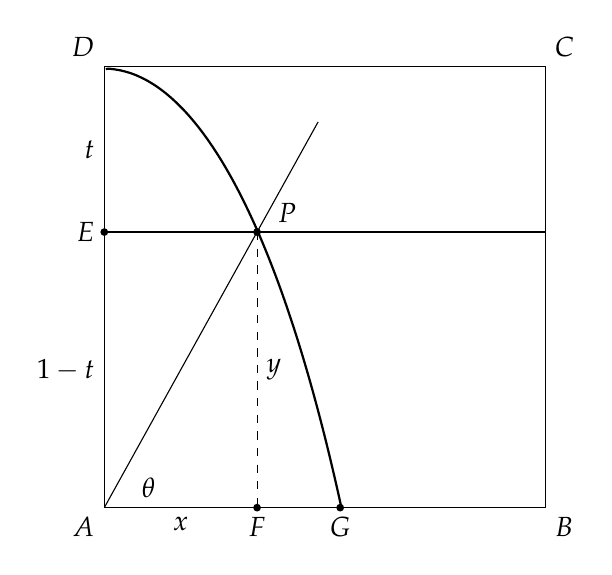
\begin{tikzpicture}[scale=.7,domain=.01:1.57,samples=100]
\draw (0,0) node[below left] {$A$} node [above right,xshift=10pt] {$\theta$} -- (8,0) node[below right] {$B$} -- (8,8) node[above right] {$C$} -- (0,8) node[above left] {$D$} -- cycle;
\draw[name path=horiz] (0,5) -- (8,5);
\draw[name path=slant] (0,0) -- (61:8);
\path[name intersections={of=horiz and slant,by=joint}];
\draw[dashed] (joint) -- node[right] {$y$} (joint |- 0,0) coordinate (f);
\path (0,0) -- node[below] {$x$} (0,0 -| joint) node[below] {$F$};
\path (0,5) node[left] {$E$} -- node[left] {$t$} (0,8);
\path (0,0) -- node[left] {$1-t$} (0,5);
\fill (joint) circle [radius=2pt] node[above right,xshift=4pt] {$P$};
\fill (f) circle [radius=2pt];
\fill (0,5) circle [radius=2pt];
\fill (4.28,0) circle [radius=2pt] node[below] {$G$};
\draw[name path=curve,thick] plot (4.3*.637*\x,{12.5*.637*\x*cot(\x r)});
\end{tikzpicture}
\end{center}

Suppose that the horizontal straightedge has moved $t$ down the $y$-axis to point $E$ and the rotating straightedge forms an angle of $\theta$ with the $x$-axis. $P$ is the intersection of the quadratrix with the horizontal straightedge, and $F$ is the projection of $P$ on the $x$-axis. What are the coordinates of quadratrix at $P$? Clearly, $y=PF=EA=1-t$. On the quadratrix, $\theta$ decreases at the same rate that $t$ increases:
\erh{0pt}
\begin{equationarray*}{rcl}
\frac{1-t}{1} &=& \frac{\theta}{\pi/2}\\
&&\\
\theta &=&\frac{\pi}{2}(1-t)\,.
\end{equationarray*}
Check if this makes sense: when $t=0$, $\theta=\pi/2$ and when $t=1$, $\theta=0$.

The $x$-coordinate of $P$ follows from trigonometry:
\[
\tan \theta = \frac{y}{x}\,.
\]
which gives:
\[
x = \frac{y}{\tan\theta}=y\cot\theta=y\cot \frac{\pi}{2}(1-t)=y\cot \frac{\pi}{2}y\,.
\]
We usually express a function as $y=f(x)$ but it can also be expressed as $x=f(y)$. Let us compute the $x$-coordinate of the point $G$, the intersection of the quadratrix with the $x$-axis. We can't simply plug in $y=0$ because $\cot 0$ is not defined, but we might get lucky by computing the limit of $x$ as $y$ goes to $0$:
\[
x = y\cot \frac{\pi}{2}y = \frac{2}{\pi}\cdot \frac{\pi}{2}y\cot \frac{\pi}{2}y\,.
\]
For convenience, perform a change of variable $z=\disfrac{\pi}{2}y$ and compute the limit:
\[
\lim_{z\rightarrow 0} z\cot z = \lim_{z\rightarrow 0} \frac{z\cos z}{\sin z} = \lim_{z\rightarrow 0} \frac{\cos z}{\disfrac{\sin z}{z}} = \frac{\cos 0}{1} = 1\,,
\]
using the well-known fact that $\displaystyle\lim_{z\rightarrow 0} \frac{\sin z}{z}=1$.
Therefore, as $y\rightarrow 0$:
\[
x \rightarrow \frac{2}{\pi}\cdot \lim_{y\rightarrow 0}\frac{\pi}{2}y\cot \frac{\pi}{2}y = \frac{2}{\pi}\cdot 1 = \frac{2}{\pi}\,.
\]
Using the quadratrix we have constructed a line segment $AG$ whose length is $x=\displaystyle\frac{2}{\pi}$. With an ordinary straightedge and compass it is easy to construct a line segment of length $\sqrt{\disfrac{2}{x}}=\sqrt{\pi}$ and then construct a square whose area is $\pi$.




\tikzsetfigurename{square-a-circle}
% !TeX root = constructions.tex

\chapter{How to (Almost) Square a Circle}\label{c.squaring}

\section{Approximations to $\pi$}\label{s.square-intro}

To square a circle the length $\sqrt{\pi}$ must be constructed, however, $\pi$ is \emph{transcendental}, meaning that it is not the solution of any algebraic equation.

This chapter brings three constructions of approximations to $\pi$. The following table shows the formulas of the lengths that are constructed, their approximate values, the difference between these values and the value of $\pi$, and the error in meters that results if the approximation is used to compute the circumference of the earth given that its radius is $6378$ km.
\[
\renewcommand{\arraystretch}{2.2}
\begin{array}{|l|c|c|c|c|}
\hline
\textrm{Construction} & \textrm{Formula} &\textrm{Value} & \textrm{Difference} & \textrm{Error (m)}\\\hline
\pi & & 3.14159265359 & - & -\\\hline
\textrm{Kochansky} & \sqrt{\disfrac{40}{3}-2\sqrt{3}}&
  3.14153338705 & 5.932 \times 10^{-5} & 756\\\hline
\textrm{Ramanujan}\; 1 & \disfrac{355}{113} &
  3.14159292035 &2.667  \times 10^{-7}&3.4\\\hline
\textrm{Ramanujan}\; 2 &\left(9^2+\disfrac{19^2}{22}\right)^{1/4}&
  3.14159265258 & 1.007 \times 10^{-9}& 0.013\\\hline
\end{array}
\]
Kochansky's construction from $1685$ can be found in \cite{bold}.

Ramanujan's constructions from $1913$ can be found in \cite{ramanujan1,ramanujan2}.

In the constructions in this chapter we need to divide a line segment into three parts; here we show how the division of two lengths can be constructed. Given a line segment of length $1$ and line segments of lengths $a,b$, by similar triangles:
\[
\disfrac{1}{b}=\disfrac{\overline{OD}}{a}\,,
\]
so $\overline{OD}=\disfrac{a}{b}$.

\begin{center}
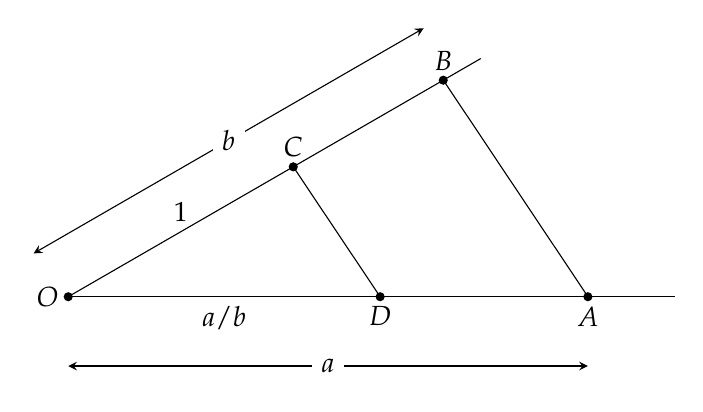
\begin{tikzpicture}[scale=1.1]
%\clip (-.6,-1) rectangle (4,3);
\draw[name path=horz] (0,0) coordinate (o) -- (7,0);
\fill (o) circle(1.5pt) node[left] {$O$};
\fill (6,0) circle(1.5pt) coordinate (a) node[below] {$A$};
\draw (0,0) -- (30:5.5);
\fill (30:3) circle(1.5pt) coordinate (c) node[above] {$C$};
\fill (30:5) circle(1.5pt) coordinate (b) node[above] {$B$};
\draw (a) -- (b);
\path[name path=par] (c) -- +($(a)-(b)$);
\path[name intersections={of=par and horz,by=d}];
\fill (d) circle(1.5pt) node[below] {$D$};
\draw (c) -- (d);
\draw[<->] (-.4,.5) -- node[fill=white] {$b$} +(30:5.2);
\path (o) -- node[above] {$1$} (c);
\draw[<->] (0,-.8) -- node[fill=white] {$a$} +(6,0);
\path (o) -- node[below] {$a/b$} (d);
\end{tikzpicture}
\end{center}

\newpage


%%%%%%%%%%%%%%%%%%%%%%%%%%%%%%%%%%%%%%%%%%%%%%%%%%%%%%%%%%%%%%%%%%%

\section{Kochansky's construction}

\subsection{The construction}

Construct three circles:
\begin{enumerate}
\item Construct a unit circle centered at $O$, let $\overline{AB}$ be a diameter and construct a tangent to the circle at $A$.
\item Construct a unit circle centered at $A$. Its intersection with the first circle is $C$.\footnote{For the second and third circles, the diagram only shows the arc that intersects the previous circle.}
\item Construct a unit circle centered at $C$. Its intersection with the second circle is $D$. 
\end{enumerate}
Construct $\overline{OD}$ and denote its intersection with the tangent by $E$.

From $E$ construct $F,G,H$, each at distance $1$ from the previous point; then $\overline{AH}=3-\overline{EA}$.

Construct $\overline{BH}$.

Claim: $\overline{BH}=\sqrt{\disfrac{40}{3}-2\sqrt{3}}\approx \pi$.
\begin{center}
\begin{tikzpicture}[scale=.9]
% Scale at 4

% Coordinates of circle
\coordinate (O) at (0,0);
\coordinate (A) at (0,-4);
\coordinate (B) at (0,4);
\fill (O) circle(2pt) node[above right] {$O$};
\fill (A) circle(2pt) node[below right] {$A$};
\fill (B) circle(2pt) node[above right] {$B$};
\draw (A) rectangle +(12pt,12pt);

% Draw circle and diameter
\node [draw,circle through=(A),name path=circle] at (O) {};
\draw (A) --  node[right] {$1$} (O) -- node[right] {$1$} (B);

% Draw tangent at A
\draw[name path=tangent] ($(A)+(-4.5,0)$) -- ($(A)+(10.5,0)$);

% Draw arc centered at A which intersects circle at C
\draw[name path=Aarc] (O)
   arc [start angle=90,end angle=220,radius=4];
\path[name intersections={of=circle and Aarc,by=C}];
\fill (C) circle(2pt) node[left,xshift=-4pt] {$C$};

% Draw arc centered at C which intersects the first arc at D
\draw[name path=Carc] ($(C)+(260:4)$)
   arc [start angle=260,end angle=280,radius=4];
\path[name intersections={of=Carc and Aarc,by=D}];
\fill (D) circle(2pt) node[below left] {$D$};

% Draw O--D which intersects the tangent at E
\draw[name path=OD] (O) -- (D);
\path[name intersections={of=tangent and OD,by=E}];
\fill (E) circle(2pt) node[above left] {$E$};

% Find point H at length 3 from E
\coordinate (F) at ($(E)+(4,0)$);
\fill (F) circle(2pt) node[above right,xshift=4pt] {$F$};
\coordinate (G) at ($(F)+(4,0)$);
\fill (G) circle(2pt) node[above] {$G$};
\coordinate (H) at ($(G)+(4,0)$);
\fill (H) circle(2pt) node[above] {$H$};

% Draw BH of length approximately pi
\draw (B) -- (H);

\draw[<->] ($(E)+(0,-.8)$) -- node[fill=white] {$1$} ($(F)+(0,-.8)$);
\draw[<->] ($(F)+(0,-.8)$) -- node[fill=white] {$1$} ($(G)+(0,-.8)$);
\draw[<->] ($(G)+(0,-.8)$) -- node[fill=white] {$1$} ($(H)+(0,-.8)$);

\end{tikzpicture}
\end{center}

\newpage

\subsection{The proof}

Extract the following diagram from the first one. Dashed line segments have been added. Since all the circles are unit circles, it is easy to see that the length of each dashed line segment is $1$. It follows that  $\overline{AOCD}$ is a rhombus so its diagonals are perpendicular to and bisect each other at $K$ and $\overline{AK}=\frac{1}{2}$.
\begin{center}
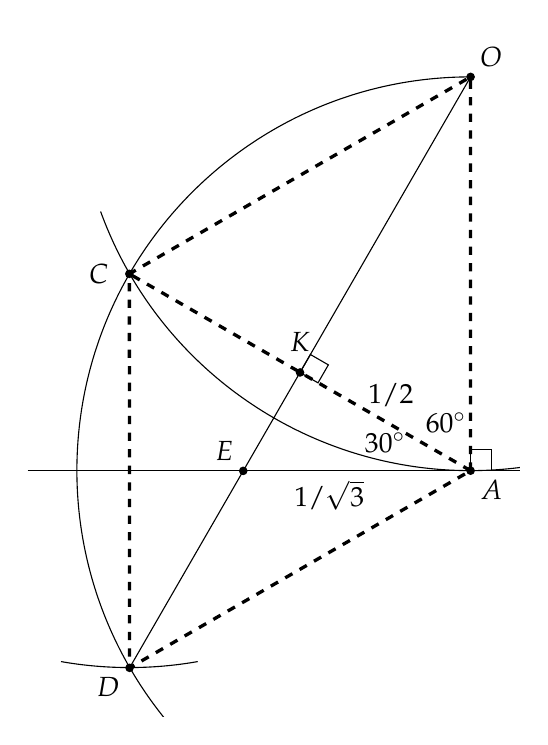
\begin{tikzpicture}[scale=1.25]
% Scale at 4

\clip (-4.5,-6.5) rectangle +(5,7);
% Coordinates of circle
\coordinate (O) at (0,0);
\coordinate (A) at (0,-4);
\coordinate (B) at (0,4);

% Draw circle
\node [circle through=(A),name path=circle] at (O) {};
\draw ($(O)+(200:4)$) arc [start angle=200,end angle=280,radius=4];

% Draw tangent at A
\draw[name path=tangent] ($(A)+(-4.5,0)$) -- ($(A)+(10.5,0)$);
\draw (A) rectangle +(6pt,6pt);

% Draw arc centered at O which intersects circle at C
\draw[name path=Aarc] (O)
   arc [start angle=90,end angle=220,radius=4];
\path[name intersections={of=circle and Aarc,by=C}];

% Draw arc centered at C which intersects the first arc at D
\draw[name path=Carc] ($(C)+(260:4)$)
   arc [start angle=260,end angle=280,radius=4];
\path[name intersections={of=Carc and Aarc,by=D}];

% Draw O--D which intersects the tangent at E
\draw[name path=OD] (O) -- (D);
\path[name intersections={of=tangent and OD,by=E}];

% Find point H at length 3 from E
\coordinate (F) at ($(E)+(4,0)$);
\coordinate (G) at ($(F)+(4,0)$);
\coordinate (H) at ($(G)+(4,0)$);

% Draw BH of length approximately pi
\draw (B) -- (H);

\draw[very thick,dashed] (A) -- (O) -- (C) -- (D) -- cycle;
\draw[very thick,dashed,name path=AC] (A) -- (C);

\node[above left,yshift=10pt,xshift=2pt] at (A) {$60^\circ$};
\node[left,yshift=10pt,xshift=-20pt] at (A) {$30^\circ$};

\path[name intersections={of=AC and OD,by=K}];
\draw[rotate=-30] (K) rectangle +(6pt,6pt);

\path (A) -- node[above,xshift=2pt,yshift=2pt] {$1/2$} (K);
\path (A) -- node[below,xshift=-10pt] {$1/\sqrt{3}$} (E);

\fill (O) circle(1.25pt) node[above right] {$O$};
\fill (A) circle(1.25pt) node[below right] {$A$};
\fill (B) circle(1.25pt) node[above right] {$B$};
\fill (C) circle(1.25pt) node[left,xshift=-4pt] {$C$};
\fill (D) circle(1.25pt) node[below left] {$D$};
\fill (E) circle(1.25pt) node[above left] {$E$};
\fill (F) circle(1.25pt) node[above right,xshift=4pt] {$F$};
\fill (G) circle(1.25pt) node[above] {$G$};
\fill (H) circle(1.25pt) node[above] {$H$};
\fill (K) circle(1.25pt) node[above,yshift=4pt] {$K$};
\end{tikzpicture}
\end{center}
The diagonal $\overline{AC}$ forms two equilateral triangles $\triangle OAC, \triangle DAC$ so $\angle OAC=60^\circ$. Since tangent forms a right angle with the radius $\overline{OA}$, $\angle KAE=30^\circ$. Now:
\begin{displaymath}
\renewcommand{\arraystretch}{1.5}
\begin{array}{lcl}
\disfrac{1/2}{\overline{EA}}&=&
\cos 30^\circ=\disfrac{\sqrt{3}}{2}\\
\overline{EA}&=&\disfrac{1}{\sqrt{3}}\\
\overline{AH}&=&3-\overline{EA}=\left(3-\disfrac{1}{\sqrt{3}}\right)
=\disfrac{3\sqrt{3}-1}{\sqrt{3}}\\
\end{array}
\end{displaymath}

Returning to the first diagram, we see that $\triangle ABH$ is a right triangle:
\begin{displaymath}
\renewcommand{\arraystretch}{2}
\begin{array}{lcl}
\overline{BH}^2&=&\overline{OB}^2+\overline{AH}^2\\
&=&4+\disfrac{9\cdot 3 -6\sqrt{3}+1}{3}=\disfrac{40}{3}-2\sqrt{3}\\
\overline{BH}&=&\sqrt{\disfrac{40}{3}-2\sqrt{3}}\approx 3.141533387\approx \pi\,.
\end{array}
\end{displaymath}

\newpage


%%%%%%%%%%%%%%%%%%%%%%%%%%%%%%%%%%%%%%%%%%%%%%%%%%%%%%%%%%%%%%%%%%%



\section{Ramanujan's first construction}


\subsection{The construction}

Construct a unit circle centered at $O$ and let $\overline{PR}$ be a diameter. 

$H$ bisects $\overline{PO}$ and $T$ trisects $\overline{RO}$. 

Construct a perpendicular at $T$ that intersects the circle at $Q$.

Construct a chord $\overline{RS}=\overline{QT}$.

Construct $\overline{PS}$.

Construct a line parallel to $\overline{RS}$ from $T$ that intersects $\overline{PS}$ at $N$.

Construct a line parallel to $\overline{RS}$ from $O$ that intersects $\overline{PS}$ at $M$.

Construct the chord $\overline{PK}=\overline{PM}$.

Construct the tangent at $P$ of length $\overline{PL}=\overline{MN}$.

Connect the points $K,L,R$.

Find point $C$ such that $\overline{RC}$ is equal to $\overline{RH}$.

Construct $\overline{CD}$ parallel to $\overline{KL}$ that intersects $\overline{LR}$ at $D$. 

Claim: $\overline{RD}^2=\disfrac{355}{113}\approx \pi$.


\begin{center}
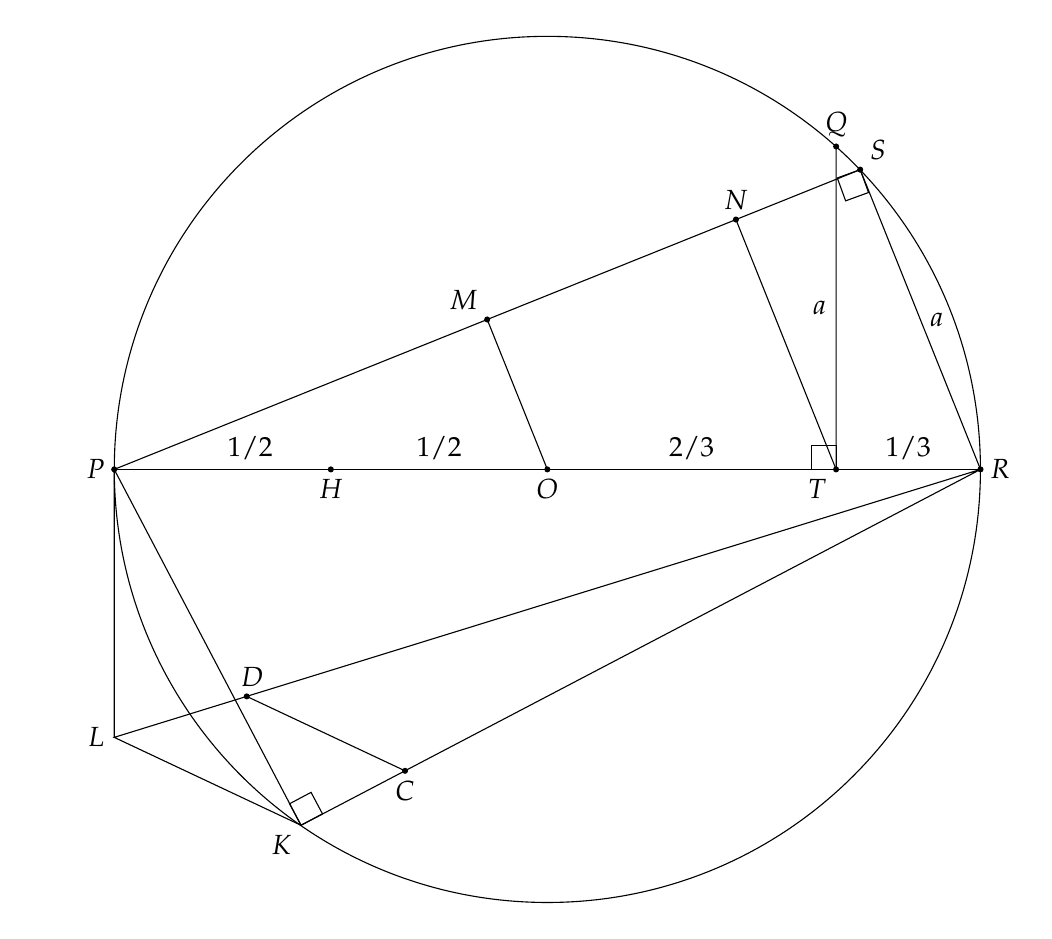
\begin{tikzpicture}[scale=1.1,align=left]
\clip (-6,-5.1) rectangle +(11.5,10.2);
% Draw circle and horizontal diameter
\draw[name path=circle] (0,0)  coordinate (o) node[below] {$O$} circle[radius=5cm];
\draw (-5,0) coordinate (p) node[left] {$P$} -- (5,0) coordinate (r) node[right] {$R$};
\fill (o) circle (1pt);
\fill (p) circle (1pt);
\fill (r) circle (1pt);
\fill (-2.5,0) coordinate (h) node[below] {$H$} circle (1pt);
\fill (10/3,0) coordinate (t) node[below left] {$T$} circle (1pt);
\path (p) -- node[above,xshift=10pt] {$1/2$} (h) -- node[above] {$1/2$} (o) -- node[above] {$2/3$} (t) -- node[above] {$1/3$} (r);

% Draw perpendicular TQ
\path[name path=tq] (t) -- +(0,5);
\path[name intersections={of=tq and circle,by=q}];
\draw (t) -- node[left] {$a$} (q) node[above] {$Q$};
\fill (q) circle (1pt);

% Draw chord RS and line PS
\path[name path=tq] (t) -- +(0,5);
\path[name intersections={of=tq and circle,by=q}];
\path[name path=rcirc] (r) let \p1 = ($ (t) - (q) $) in circle ({veclen(\x1,\y1)});
\path[name intersections={of=rcirc and circle,by=s}];
\draw (r) -- node[right] {$a$} (s);
\fill (s) node[above right] {$S$} circle (1pt);
\draw[name path=ps] (p) -- (s);

% Draw TN
\path[name path=tn] (t) -- +($(s)-(r)$);
\path[name intersections={of=ps and tn,by=n}];
\draw (t) -- (n);
\fill (n) node[above] {$N$} circle (1pt);

% Draw OM
\path[name path=om] (o) -- +($(s)-(r)$);
\path[name intersections={of=ps and om,by=m}];
\draw (o) -- (m);
\fill (m) node[above left] {$M$} circle (1pt);
\path (p) -- (m);
\path (m) -- (n);

% Draw chord PK
\draw (p) -- +(-62.3:4.64) coordinate (k) node[below left] {$K$};

% Draw tangent PL
\draw let \p1 = ($ (m) - (n) $), \n1 = {veclen(\x1,\y1)} in (p) -- (-5,-\n1) coordinate (l) node[left] {$L$};

% Connect L and K to R
\draw (r) -- (l) -- (k) -- cycle;

% Find point C on RK
\coordinate (c) at ($(r)!7.5cm!(k)$);
\path (r) -- (c);
\fill (c) node[below] {$C$} circle (1pt);

% Draw CD
\path[name path=cd] (c) -- +($(l)-(k)$);
\path[name path=lr] (l) -- (r);
\path[name intersections={of=cd and lr,by=d}];
\draw (c) -- (d);
\fill (d) node[above,xshift=2pt] {$D$} circle (1pt);
\path (r) -- (d);

\draw[rotate=90] (t) rectangle +(8pt,8pt);
\draw[rotate=-160] (s) rectangle +(8pt,8pt);
\draw[rotate=28] (k) rectangle +(8pt,8pt);
\end{tikzpicture}
\end{center}

\newpage

\subsection{The proof}

By Pythagoras' theorem on $\triangle QOT$:
\[
\overline{QT} = \sqrt{1^2-\left(\frac{2}{3}\right)^2}=\frac{\sqrt{5}}{3}\,.
\]
$\triangle PSR$ is a right triangle because it subtends a diameter. By Pythagoras theorem:
\[
\overline{PS} = \sqrt{2^2-\left(\frac{\sqrt{5}}{3}\right)^2}=\sqrt{4-\frac{5}{9}}=\frac{\sqrt{31}}{3}\,.
\]
$\triangle MPO\sim \triangle SPR$ so:
\begin{form}{2.2}
\disfrac{\overline{PM}}{\overline{PO}}&=&\disfrac{\overline{PS}}{\overline{PR}}\\
\disfrac{\overline{PM}}{1}&=&\disfrac{\sqrt{31}/3}{2}\\
\overline{PM}&=&\disfrac{\sqrt{31}}{6}\\
\overline{PK}&=&\overline{PM}=\disfrac{\sqrt{31}}{6}\,.
\end{form}
$\triangle NPT\sim \triangle SPR$ so:

\begin{form}{2.2}
\disfrac{\overline{PN}}{\overline{PT}}&=&\disfrac{\overline{PS}}{\overline{PR}}\\
\disfrac{\overline{PN}}{5/3}&=&\disfrac{\sqrt{31}/3}{2}\\
\overline{PN}&=&\disfrac{5\sqrt{31}}{18}\\
\overline{MN}&=&\overline{PN}-\overline{PM}=\sqrt{31}\left(\disfrac{5}{18}-\disfrac{1}{6}\right) = \disfrac{\sqrt{31}}{9}\\
\overline{PL}&=&\overline{MN}=\disfrac{\sqrt{31}}{9}\,.
\end{form}

$\triangle PKR$ is a right triangle because it subtends a diameter. By Pythagoras's theorem:
\[
\overline{RK}=\sqrt{2^2-\left(\frac{\sqrt{31}}{6}\right)^2} = \frac{\sqrt{113}}{6}\,.
\]

$\triangle PLR$ is a right triangle because it $\overline{PL}$ is a tangent. By Pythagoras's theorem:
\[
\overline{RL}=\sqrt{2^2+\left(\frac{\sqrt{31}}{9}\right)^2} = \frac{\sqrt{355}}{9}\,.
\]

\newpage

$\overline{RC}=\overline{RH}=\displaystyle\frac{1}{3}+\frac{2}{3}+\frac{1}{2}=\frac{3}{2}$. Since $\overline{CD}$ is parallel to $\overline{LK}$, by similar triangles:
\begin{form}{2.2}
\disfrac{\overline{RD}}{\overline{RC}}&=&\disfrac{\overline{RL}}{\overline{RK}}\\
\disfrac{\overline{RD}}{3/2}&=&\disfrac{\sqrt{355}/9}{\sqrt{113}/6}\\
\overline{RD}&=&\sqrt{\disfrac{355}{113}}\,.
\end{form}

Here is the construction with line segments labeled with their lengths:

\begin{center}
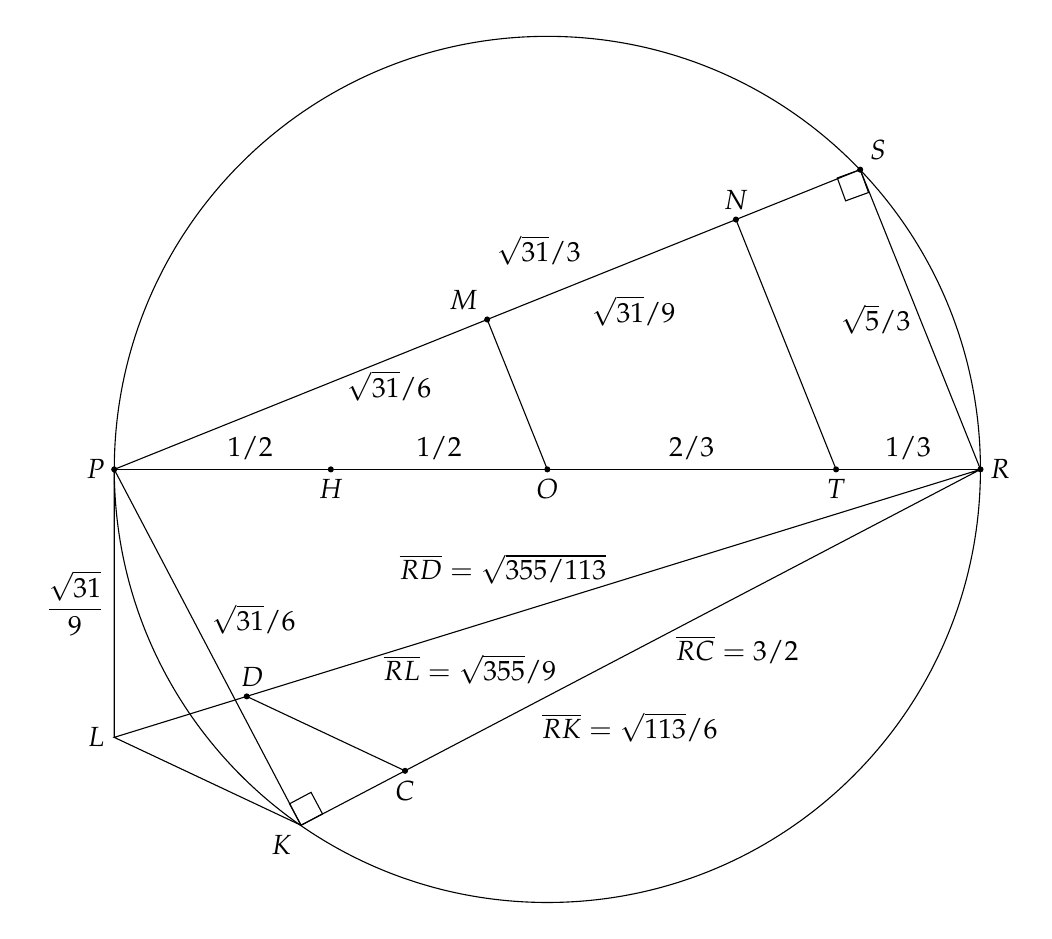
\begin{tikzpicture}[scale=1.1,align=left]
\clip (-6,-5.1) rectangle +(11.5,10.2);
% Draw circle and horizontal diameter
\draw[name path=circle] (0,0)  coordinate (o) node[below] {$O$} circle[radius=5cm];
\draw (-5,0) coordinate (p) node[left] {$P$} -- (5,0) coordinate (r) node[right] {$R$};
\fill (o) circle (1pt);
\fill (p) circle (1pt);
\fill (r) circle (1pt);
\fill (-2.5,0) coordinate (h) node[below] {$H$} circle (1pt);
\fill (10/3,0) coordinate (t) node[below] {$T$} circle (1pt);
\path (p) -- node[above,xshift=10pt] {$1/2$} (h) -- node[above] {$1/2$} (o) -- node[above] {$2/3$} (t) -- node[above] {$1/3$} (r);
% Draw chord RS and line PS
\path[name path=tq] (t) -- +(0,5);
\path[name intersections={of=tq and circle,by=q}];
\path[name path=rcirc] (r) let \p1 = ($ (t) - (q) $) in circle ({veclen(\x1,\y1)});
\path[name intersections={of=rcirc and circle,by=s}];
\draw (r) -- node[left] {$\sqrt{5}/3$} (s);
\fill (s) node[above right] {$S$} circle (1pt);
\draw[name path=ps] (p) -- node[above right,yshift=16pt] {$\sqrt{31}/3$} (s);
% Draw TN
\path[name path=tn] (t) -- +($(s)-(r)$);
\path[name intersections={of=ps and tn,by=n}];
\draw (t) -- (n);
\fill (n) node[above] {$N$} circle (1pt);
% Draw OM
\path[name path=om] (o) -- +($(s)-(r)$);
\path[name intersections={of=ps and om,by=m}];
\draw (o) -- (m);
\fill (m) node[above left] {$M$} circle (1pt);
\path (p) -- node[below,xshift=32pt,yshift=12pt] {$\sqrt{31}/6$} (m);
\path (m) -- node[below,xshift=8pt,yshift=-6pt] {$\sqrt{31}/9$} (n);
% Draw chord PK
\draw (p) -- node[right,xshift=-2pt,yshift=10pt] {$\sqrt{31}/6$} +(-62.3:4.64) coordinate (k) node[below left] {$K$};
% Draw tangent PL
\draw let \p1 = ($ (m) - (n) $), \n1 = {veclen(\x1,\y1)} in (p) -- node[left] {$\disfrac{\sqrt{31}}{9}$} (-5,-\n1) coordinate (l) node[left] {$L$};
% Connect L and K to R
\draw (r) -- (l) -- (k) -- cycle;
% Find point C on RK
\coordinate (c) at ($(r)!7.5cm!(k)$);
%\path (r) -- node[below,yshift=-16pt] {$RC=3/2$\\$RK=\sqrt{113}/6$} (c);
\path (r) -- node[below,xshift=16pt,yshift=-2pt] {$\overline{RC}=3/2$} (c);
\path (r) -- node[below,xshift=-4pt,yshift=-20pt] {$\overline{RK}=\sqrt{113}/6$} (k);
\fill (c) node[below] {$C$} circle (1pt);
% Draw CD
\path[name path=cd] (c) -- +($(l)-(k)$);
\path[name path=lr] (l) -- (r);
\path[name intersections={of=cd and lr,by=d}];
\draw (c) -- (d);
\fill (d) node[above,xshift=2pt] {$D$} circle (1pt);
%\path (r) -- node[above,xshift=-40pt,yshift=-8pt] {$RD=\sqrt{355/113}$\\$RL=\sqrt{355}/9$} (d);
\path (r) -- node[above,xshift=-40pt,yshift=-4pt] {$\overline{RD}=\sqrt{355/113}$} (d);
\path (r) -- node[below,xshift=-28pt,yshift=-15pt] {$\overline{RL}=\sqrt{355}/9$} (l);
\draw[rotate=28] (k) rectangle +(8pt,8pt);
\draw[rotate=-160] (s) rectangle +(8pt,8pt);
\end{tikzpicture}
\end{center}

\bigskip

The value $\disfrac{355}{113}$ could be constructed by constructing two line segments of length $355$ and $113$ and then using the division construction shown in Section~\ref{s.square-intro}, but that is rather tedious!

\newpage

%%%%%%%%%%%%%%%%%%%%%%%%%%%%%%%%%%%%%%%%%%%%%%%%%%%%%%%%%%%%

\section{Ramanujan's second approximation}

\subsection{The construction}

Construct a unit circle centered at $O$ with diameter $\overline{AB}$, and let $C$ be the intersection of the perpendicular at $O$ with the circle.

Trisect $\overline{AO}$ so that $\overline{AT}=1/3$ and $\overline{TO}=2/3$.

Construct $\overline{BC}$ and find points $M,N$ such that $\overline{CM}=\overline{MN}=\overline{AT}=1/3$.

Construct $\overline{AM}$ and $\overline{AN}$ and let $P$ be the point on $\overline{AN}$ such that $\overline{AP}=\overline{AM}$.

From $P$ construct a line parallel to $\overline{MN}$ that intersects $\overline{AM}$ at $Q$.

Construct $\overline{OQ}$ and then from $T$ construct a line parallel to $\overline{OQ}$ that intersects $\overline{AM}$ at $R$.

Construct a line segment $\overline{AS}$ tangent to $A$ of length $\overline{AR}$.

Construct $\overline{SO}$.

Claim: $3\sqrt{\overline{SO}}=\left(9^2+\disfrac{19^2}{22}\right)^{\frac{1}{4}}\approx \pi$.

\begin{center}
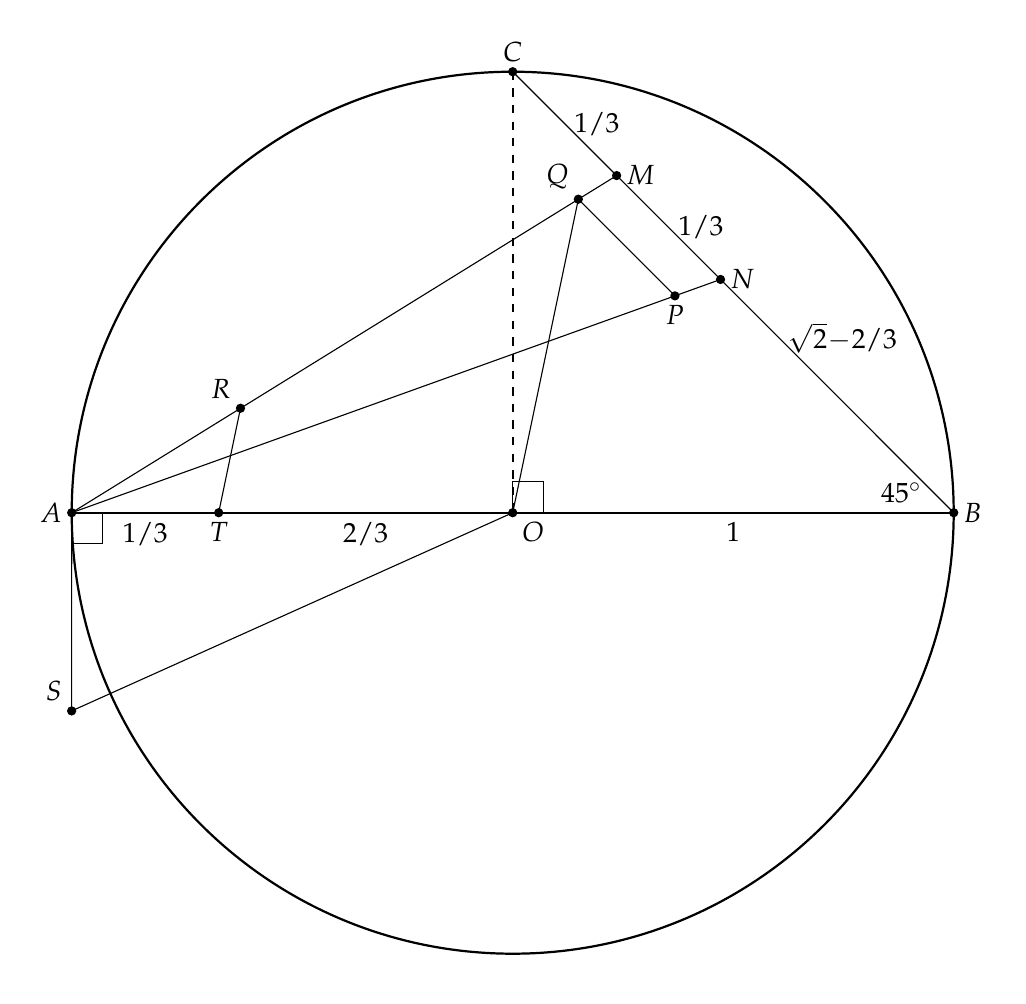
\begin{tikzpicture}[scale=1.4]
\clip (-4.4,-4.2) rectangle +(8.8,8.6);
% Scale at 4

% Coordinates of circle
\coordinate (O) at (0,0);
\coordinate (A) at (-4,0);
\coordinate (B) at (4,0);
\coordinate (C) at (0,4);

% Draw circle and diameter
\node [thick,draw,circle through=(A),name path=circle] at (O) {};
\draw [thick] (A) -- (B);
\draw [thick,dashed] (C) -- (O);
\draw (O) rectangle +(8pt,8pt);
\draw[rotate=-90] (A) rectangle +(8pt,8pt);

\coordinate (T) at (-2.667,0);
\path (A) -- node[below] {$1/3$} (T);
\path (T) -- node[below] {$2/3$} (O);
\path (O) -- node[below] {$1$} (B);

\draw (C) -- node[right] {$1/3$} +(-45:1.333) coordinate (M);
\draw (M) -- node[right] {$1/3$} +(-45:1.333) coordinate (N);
\draw (N) -- node[near start,right] {$\sqrt{2}\!-\!2/3$}(B);

\draw[name path=AM] (A) -- (M);
\draw[name path=AN] (A) -- (N);

\node [circle through=(M),name path=AMcircle] at (A) {};

\path[name intersections={of=AMcircle and AN,by=P}];

\path[name path=PQ] (P) -- +(135:2);
\path[name intersections={of=PQ and AM,by=Q}];
\draw (P) -- (Q) -- (O);

\path[name path=QT] (T) -- ($(Q)+(-2.667,0)$) -- (Q);
\path[name intersections={of=QT and AM,by=R}];
\draw (T) -- (R);

\node [circle through=(R),name path=ARcircle] at (A) {};
\path[name path=AS] (A) -- ($(A)+(0,-2.5)$);
\path[name intersections={of=ARcircle and AS,by=S}];
\draw (A) -- (S);

\draw (S) -- (O);

\fill (O) circle(1.2pt) node[below right] {$O$};
\fill (A) circle(1.2pt) node[left] {$A$};
\fill (B) circle(1.2pt) node[right] {$B$} node[above left,xshift=-8pt] {$45^\circ$};
\fill (C) circle(1.2pt) node[above] {$C$};
\fill (T) circle(1.2pt) node[below] {$T$};
\fill (M) circle(1.2pt) node[right] {$M$};
\fill (N) circle(1.2pt) node[right] {$N$};
\fill (P) circle(1.2pt) node[below] {$P$};
\fill (Q) circle(1.2pt) node[above left] {$Q$};
\fill (R) circle(1.2pt) node[above left] {$R$};
\fill (S) circle(1.2pt) node[above left] {$S$};

\end{tikzpicture}
\end{center}

\newpage

\subsection{The proof}

$\triangle COB$ is a right triangle, $\overline{OB}=\overline{OC}=1$, 	so by Pythagoras' theorem $\overline{CB}=\sqrt{2}$ and $\overline{NB}=\sqrt{2}-2/3$. The triangle is isoceles so $\angle NBA =\angle MBA=45^\circ$.

We use the law of cosines on $\triangle NBA$ to compute $\overline{AN}$:
\begin{form}{2}
\overline{AN}^2&=&\overline{BA}^2 + \overline{BN}^2-2\cdot\overline{BA}\cdot\overline{BN}\cdot\cos \angle NBA\\
&=&2^2+\left(\sqrt{2}-\disfrac{2}{3}\right)^2-2\cdot 2 \cdot \left(\sqrt{2}-\disfrac{2}{3}\right)\cdot \disfrac{\sqrt{2}}{2}\\
&=&\left(4+2+\disfrac{4}{9}-4\right) + \sqrt{2}\cdot \left(-\disfrac{4}{3}+\disfrac{4}{3}\right)=\disfrac{22}{9}\\
\overline{AN}&=&\sqrt{\disfrac{22}{9}}\,.
\end{form}

Similarly, we use the law of cosines on $\triangle MBA$ to compute $\overline{AM}$:
\begin{form}{2}
\overline{AM}^2&=&\overline{BA}^2 + \overline{BM}^2-2\cdot\overline{BA}\cdot\overline{BM}\cdot\cos \angle MBA\\
&=&2^2+\left(\sqrt{2}-\disfrac{1}{3}\right)^2-2\cdot 2 \cdot \left(\sqrt{2}-\disfrac{1}{3}\right)\cdot \disfrac{\sqrt{2}}{2}\\
&=&\left(4+2+\disfrac{1}{9}-4\right) + \sqrt{2}\cdot \left(-\disfrac{2}{3}+\disfrac{2}{3}\right)=\disfrac{19}{9}\\
\overline{AM}&=&\sqrt{\disfrac{19}{9}}\,.
\end{form}

By construction $\overline{QP}\| \overline{MN}$ so
$\triangle MAN\sim \triangle QAP$, and by construction $\overline{AP}=\overline{AM}$ giving:
\begin{form}{2.4}
\disfrac{\overline{AQ}}{\overline{AM}}&=&\disfrac{\overline{AP}}{\overline{AN}}=\disfrac{\overline{AM}}{\overline{AN}}\\
\overline{AQ}&=&\disfrac{\overline{AM}^2}{\overline{AN}}=\disfrac{19/9}{\sqrt{22/9}}=\disfrac{19}{3\sqrt{22}}\,.
\end{form}

By construction $\overline{TR}\| \overline{OQ}$ so
$\triangle RAT\sim \triangle QAO$ giving:
\begin{form}{2.4}
\disfrac{\overline{AR}}{\overline{AQ}}&=&\disfrac{\overline{AT}}{\overline{AO}}\\
\overline{AR}&=&\overline{AQ}\cdot\disfrac{\overline{AT}}{\overline{AO}}=\disfrac{19}{3\sqrt{22}}\cdot\disfrac{1/3}{1}=\disfrac{19}{9\sqrt{22}}\,.
\end{form}

\newpage

By construction $\overline{AS}=\overline{AR}$ and $\triangle OAS$ is a right triangle. By Pythagoras' theorem:
\begin{form}{3}
\overline{SO}&=&\sqrt{1^2+\left(\disfrac{19}{9\sqrt{22}}\right)^2}\\
3\sqrt{\overline{SO}}&=&3\left(1+\disfrac{19^2}{9^2\cdot 22}\right)^\frac{1}{4}\\
&=&\left(3^4+\disfrac{3^4\cdot 19^2}{9^2\cdot 22}\right)^\frac{1}{4}\\
&=&\left(9^2+\disfrac{19^2}{22}\right)^\frac{1}{4}\approx 3.14159265262\approx \pi\,.
\end{form}

Here is the construction with line segments labeled with their lengths:


\begin{center}
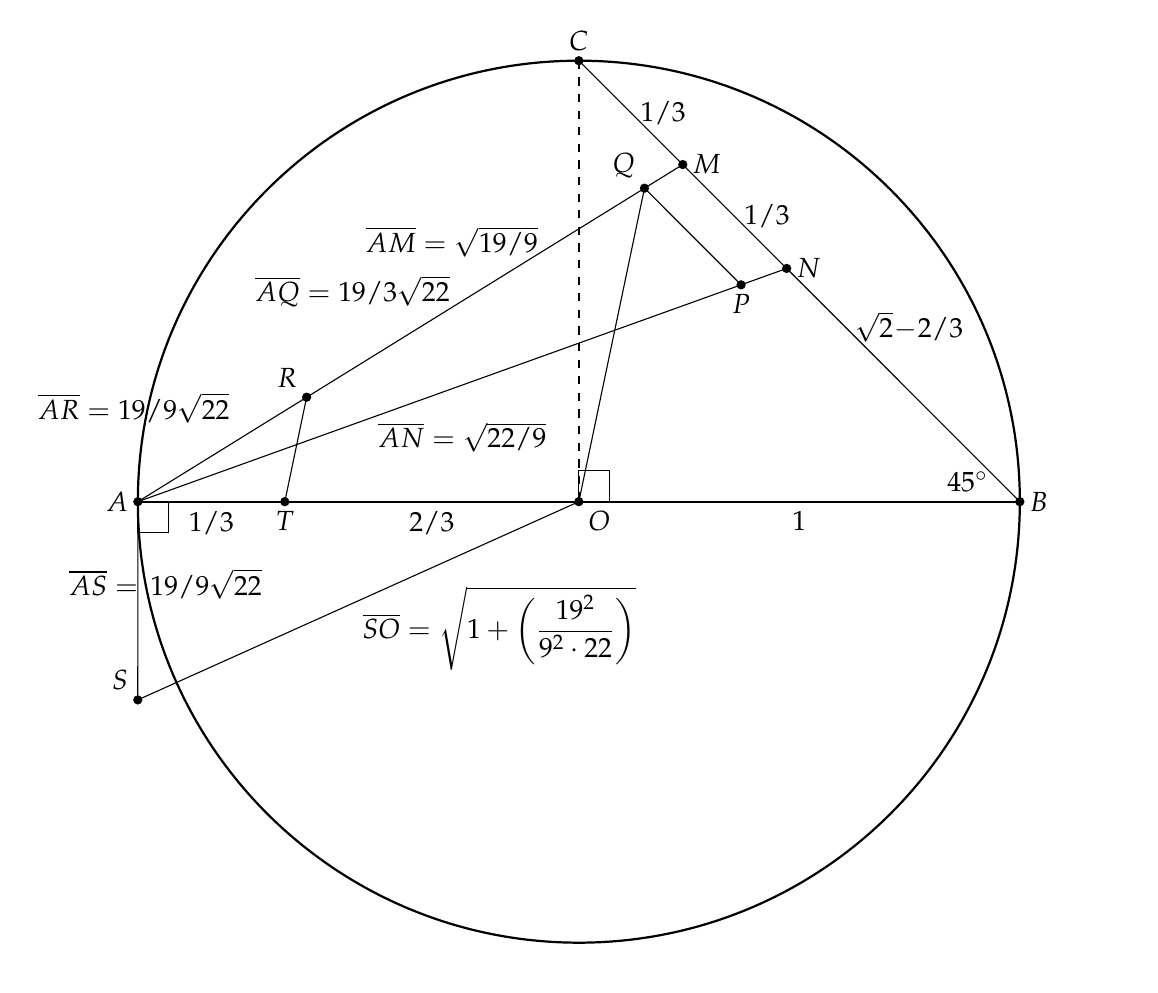
\begin{tikzpicture}[scale=1.4]
\clip (-5,-4.2) rectangle +(10,8.5);
% Scale at 4

% Coordinates of circle
\coordinate (O) at (0,0);
\coordinate (A) at (-4,0);
\coordinate (B) at (4,0);
\coordinate (C) at (0,4);

% Draw circle and diameter
\node [thick,draw,circle through=(A),name path=circle] at (O) {};
\draw [thick] (A) -- (B);
\draw [thick,dashed] (C) -- (O);
\draw (O) rectangle +(8pt,8pt);
\draw[rotate=-90] (A) rectangle +(8pt,8pt);

\coordinate (T) at (-2.667,0);
\path (A) -- node[below] {$1/3$} (T);
\path (T) -- node[below] {$2/3$} (O);
\path (O) -- node[below] {$1$} (B);

\draw (C) -- node[right] {$1/3$} +(-45:1.333) coordinate (M);
\draw (M) -- node[right] {$1/3$} +(-45:1.333) coordinate (N);
\draw (N) -- node[near start,right] {$\sqrt{2}\!-\!2/3$}(B);

\draw[name path=AM] (A) -- node[above,xshift=15pt,yshift=24pt] {$\overline{AM}=\sqrt{19/9}$} (M);
\draw[name path=AN] (A) -- node[below,yshift=-10pt] {$\overline{AN}=\sqrt{22/9}$} (N);

\node [circle through=(M),name path=AMcircle] at (A) {};

\path[name intersections={of=AMcircle and AN,by=P}];

\path[name path=PQ] (P) -- +(135:2);
\path[name intersections={of=PQ and AM,by=Q}];
\draw (P) -- (Q) -- (O);
\path (A) -- node[above,xshift=-14pt,yshift=10pt] {$\overline{AQ}=19/3\sqrt{22}$} (Q);

\path[name path=QT] (T) -- ($(Q)+(-2.667,0)$) -- (Q);
\path[name intersections={of=QT and AM,by=R}];
\draw (T) -- (R);
\path (A) -- node[above,xshift=-32pt,yshift=6pt] {$\overline{AR}=19/9\sqrt{22}$} (R);

\node [circle through=(R),name path=ARcircle] at (A) {};
\path[name path=AS] (A) -- ($(A)+(0,-2.5)$);
\path[name intersections={of=ARcircle and AS,by=S}];
\draw (A) -- node[xshift=10pt,yshift=6pt] {$\overline{AS}=\,19/9\sqrt{22}$} (S);

\draw (S) -- node[right,xshift=-2pt,yshift=-10pt] {$\overline{SO}=\sqrt{1+
  \left(\disfrac{19^2}{9^2\cdot 22}\right)}$} (O);

\fill (O) circle(1.2pt) node[below right] {$O$};
\fill (A) circle(1.2pt) node[left] {$A$};
\fill (B) circle(1.2pt) node[right] {$B$} node[above left,xshift=-8pt] {$45^\circ$};
\fill (C) circle(1.2pt) node[above] {$C$};
\fill (T) circle(1.2pt) node[below] {$T$};
\fill (M) circle(1.2pt) node[right] {$M$};
\fill (N) circle(1.2pt) node[right] {$N$};
\fill (P) circle(1.2pt) node[below] {$P$};
\fill (Q) circle(1.2pt) node[above left] {$Q$};
\fill (R) circle(1.2pt) node[above left] {$R$};
\fill (S) circle(1.2pt) node[above left] {$S$};

\end{tikzpicture}
\end{center}


\tikzsetfigurename{compass-only}
% !TeX root = constructions.tex

\chapter{A Compass is Sufficient}\label{c.compass-only}

In 1797 the Italian mathematician Lorenzo Mascheroni proved that any construction carried out with a compass and straightedge can be carried out with the compass alone! Later it came to light that the construction had already been discovered by the Danish mathematician Georg Mohr 1672. The theorem is now called the Mohr-Mascheroni Theorem.

In this chapter I present a proof of the theorem based on the proof in problem 33 of \cite{dorrie1} and reworked by  Michael Woltermann \cite{dorrie2}.\footnote{I would like to thank Woltermann for permission to use his work.} A different  proof can be found in \cite{mm}.

What does it mean to perform a construction with only a compass? The right diagram below shows the construction of an equilateral triangle using a straightedge and compass. How can we construct a triangle without the line segments $\overline{AB}, \overline{AC}, \overline{BC}$? In fact, there is no need to \emph{see} the lines. A line is defined by two points, so it is sufficient to construct the points in order to obtain a construction equivalent to the one with a straightedge (left diagram):
\begin{center}
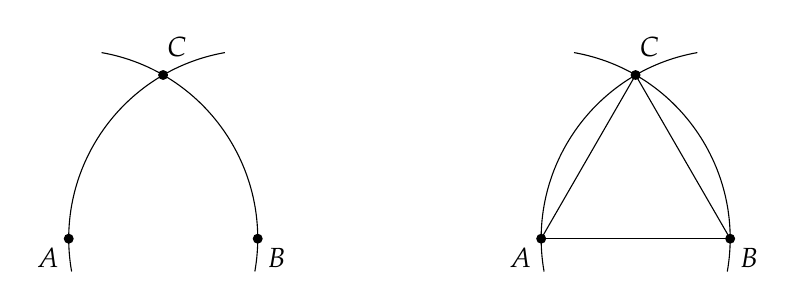
\begin{tikzpicture}[scale=0.6]
\coordinate (A) at (0,0);
\coordinate (B) at (4,0);
\path (A) node[below left] {$A$} -- (B) node[below right] {$B$};
\fill (A) circle[radius=3pt];
\fill (B) circle[radius=3pt];
\draw[name path=larc] (A) ++(-10:4cm) arc (-10:80:4cm);
\draw[name path=rarc] (B) ++(-170:4cm) arc (-170:-260:4cm);
\path [name intersections={of=larc and rarc,by={t}}];
\fill (t) node[above right,xshift=-2pt,yshift=3pt] {$C$} circle[radius=3pt];
\begin{scope}[xshift=10cm]
\coordinate (A) at (0,0);
\coordinate (B) at (4,0);
\draw (A) node[below left] {$A$} -- (B) node[below right] {$B$};
\fill (A) circle[radius=3pt];
\fill (B) circle[radius=3pt];
\draw[name path=larc] (A) ++(-10:4cm) arc (-10:80:4cm);
\draw[name path=rarc] (B) ++(-170:4cm) arc (-170:-260:4cm);
\path [name intersections={of=larc and rarc,by={t}}];
\fill (t) node[above right,xshift=-2pt,yshift=3pt] {$C$} circle[radius=3pt];
\draw (A) -- (t);
\draw (B) -- (t);
\end{scope}
\end{tikzpicture}
\end{center}
In the diagrams we will draw lines, but they are used only to understand the construction and the proof of its correctness. It is important that you convince yourself that the construction itself uses only a compass.

A construction by straightedge and compass is a sequence taken from these three operations:
\begin{itemize}
\item Find the point of intersection of two straight lines.
\item Find the point of intersection of a straight line and a circle.
\item Find the point(s) of intersection of two circles.
\end{itemize}
It is clear that the third operation can be done with only a compass. We need to show that the first two operations can be done with a compass alone.

Notation:
\begin{itemize}
\item $c(O,A)$: the circle with center $O$ through point $A$.
\item $c(O,r)$: the circle with center $O$ and radius $r$.
\item $c(O,AB)$: the circle with center $O$ and radius the length of line segment $\overline{AB}$.
\end{itemize}

First we will solve four preliminary problems (Sections~\ref{s.reflection}--\ref{s.three}). Next, we show the construction for finding the intersection of two lines (Section~\ref{s.two-lines}), and finally the construction of the intersection of a line and a circle (Section~\ref{s.line-circle}).

%%%%%%%%%%%%%%%%%%%%%%%%%%%%%%%%%%%%%%%%%%%%%%%%%%%%%%%%%%%%%%%

\section{Reflection of a point}\label{s.reflection}

\textbf{Given a line $\overline{AB}$ and a point $C$ not on $\overline{AB}$, build a point $C'$ which is a reflection of $C$ about $\overline{AB}$.}

$C'$ is a \emph{reflection} about a line segment $\overline{AB}$ if $\overline{AB}$ (or the line containing $\overline{AB}$) is the perpendicular bisector of the line $CC'$.

Construct a circle centered on $A$ passing through $C$ and circle centered on $B$ passing through $C$. The intersection of the two circles is the point $C'$ which is the reflection of $C$.
\begin{center}
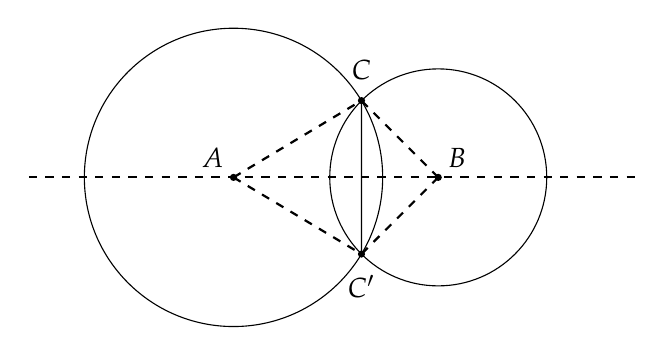
\begin{tikzpicture}[scale=.65]
\coordinate (A) at (0,0);
\coordinate (B) at (4,0);
\coordinate (C) at (2.5,1.5);
\draw[thick,dashed] ($(B)!2!(A)$) -- ($(A)!2!(B)$);
\fill (A) node[above left] {$A$} circle[radius=2pt];
\fill (B) node[above right] {$B$} circle[radius=2pt];
\fill (C) node[above,yshift=4pt] {$C$} circle[radius=2pt];
\node[draw,circle through=(C),name path=ac] at (A) {};
\node[draw,circle through=(C),name path=bc] at (B) {};
\path [name intersections={of=ac and bc,by={x1,Cp}}];
\fill (Cp) node[below,yshift=-4pt] {$C'$} circle[radius=2pt];
\draw (C) -- (Cp);
\draw[thick,dashed] (A) -- (C);
\draw[thick,dashed] (B) -- (C);
\draw[thick,dashed] (A) -- (Cp);
\draw[thick,dashed] (B) -- (Cp);
\end{tikzpicture}
\end{center}
\textbf{Proof:} $\triangle ABC \cong \triangle ABC'$ by side-side-side since $\overline{AC}, \overline{AC'}$ are radii of the same circle as are $\overline{BC}, \overline{BC'}$, and $\overline{AB}$ is a common side. Therefore, $\angle CAB = \angle C'AB$ so $\overline{AB}$ is the angle bisector of $\angle CAC'$. But $\triangle CAC'$ is an isosceles triangle and the angle bisector $\overline{AB}$ is also the perpendicular bisector of the base of $\triangle CAC'$. By definition $C'$ is the reflection of $C$ around $\overline{AB}$.

%%%%%%%%%%%%%%%%%%%%%%%%%%%%%%%%%%%%%%%%%%%%%%%%%%%%%%%%%%%%%%%

\section{Construct a circle with a given radius}\label{s.circle}

\textbf{Given points $A,B,C$, construct $c(A,BC)$.}

Construct $c(A,B)$ and $c(B,A)$ and let $X$ and $Y$ be their points of intersection.

\begin{center}
\begin{tikzpicture}[scale=.55]
\coordinate (A) at (0,1.5);
\coordinate (B) at (0,-1.5);
\coordinate (C) at (1.5,-3);
\coordinate (Cp) at (1.5,3);
\fill (A) node[above] {$A$} circle[radius=3pt];
\fill (B) node[below] {$B$} circle[radius=3pt];
\fill (C) node[below] {$C$} circle[radius=3pt];
%\fill (Cp) node[above] {$C'$} circle[radius=3pt];
\node[draw,circle through=(B),name path=ab] at (A) {};
\node[draw,circle through=(A),name path=ba] at (B) {};
\path [name intersections={of=ab and ba,by={Y,X}}];
\fill (X) node[above right,xshift=4pt] {$X$} circle[radius=3pt];
\fill (Y) node[above left,xshift=-4pt] {$Y$} circle[radius=3pt];
\draw[thick,dashed] ($(X)!2.3!(Y)$) -- ($(Y)!2!(X)$);
\end{tikzpicture}
\vspace*{-6pt}
\end{center}

\newpage

Construct $C'$, the reflection of $C$ about line $\overline{XY}$ as described in Section~\ref{s.reflection}.

\begin{center}
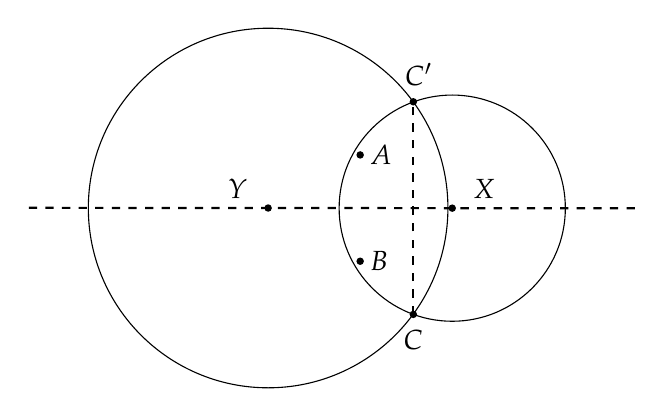
\begin{tikzpicture}[scale=.45]
\coordinate (A) at (0,1.5);
\coordinate (B) at (0,-1.5);
\coordinate (C) at (1.5,-3);
\coordinate (Cp) at (1.5,3);
\fill (A) node[right] {$A$} circle[radius=3pt];
\fill (B) node[right] {$B$} circle[radius=3pt];
\fill (C) node[below,yshift=-2pt] {$C$} circle[radius=3pt];
\fill (Cp) node[above,xshift=2pt,yshift=2pt] {$C'$} circle[radius=3pt];
\node[circle through=(B),name path=ab] at (A) {};
\node[circle through=(A),name path=ba] at (B) {};
\path [name intersections={of=ab and ba,by={Y,X}}];
\fill (X) node[above right,xshift=4pt] {$X$} circle[radius=3pt];
\fill (Y) node[above left,xshift=-4pt] {$Y$} circle[radius=3pt];
\node[draw,circle through=(C)] at (X) {};
\node[draw,circle through=(C)] at (Y) {};
\draw[thick,dashed] ($(X)!2.3!(Y)$) -- ($(Y)!2!(X)$);
%\draw (X) -- (Y) -- (C) -- (X) -- (Cp) -- (Y);
\draw[thick,dashed] (C) -- (Cp);
\end{tikzpicture}
\vspace*{-6pt}
\end{center}

$c(A,C')$ is the desired circle.

\begin{center}
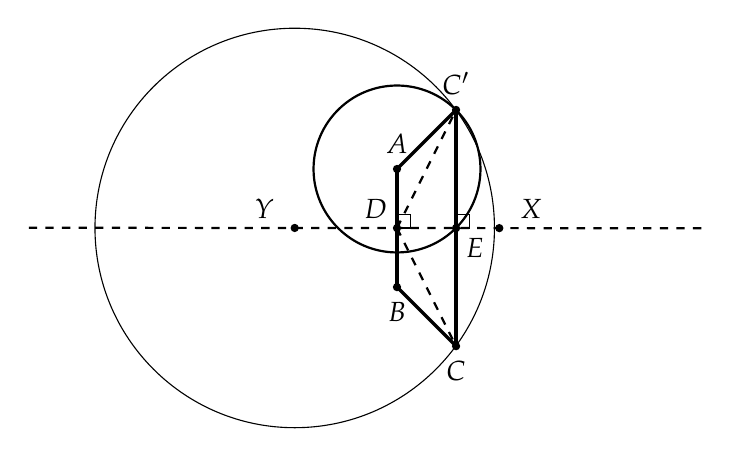
\begin{tikzpicture}[scale=.5]
\coordinate (A) at (0,1.5);
\coordinate (B) at (0,-1.5);
\coordinate (C) at (1.5,-3);
\coordinate (Cp) at (1.5,3);
\fill (A) node[above,yshift=2pt] {$A$} circle[radius=3pt];
\fill (B) node[below,yshift=-2pt] {$B$} circle[radius=3pt];
\fill (C) node[below,yshift=-2pt] {$C$} circle[radius=3pt];
\fill (Cp) node[above,yshift=2pt] {$C'$} circle[radius=3pt];
\node[circle through=(B),name path=ab] at (A) {};
\node[circle through=(A),name path=ba] at (B) {};
\path [name intersections={of=ab and ba,by={Y,X}}];
\fill (X) node[above right,xshift=4pt] {$X$} circle[radius=3pt];
\fill (Y) node[above left,xshift=-4pt] {$Y$} circle[radius=3pt];
\node[circle through=(C)] at (X) {};
\node[draw,circle through=(C)] at (Y) {};
\draw[thick,dashed] ($(X)!2.3!(Y)$) -- ($(Y)!2!(X)$);
\path[name path=xy] (X) -- (Y);
\node[draw,thick,circle through=(Cp)] at (A) {};
\draw[very thick] (A) -- (Cp);
\draw[very thick] (B) -- (C);
\draw[very thick,name path=abline] (A) -- (B);
\draw[very thick,name path=ccp] (C) -- (Cp);
\path [name intersections={of=xy and abline,by={D}}];
\path [name intersections={of=xy and ccp,by={E}}];
\fill (D) node[above left] {$D$} circle[radius=3pt];
\fill (E) node[below right] {$E$} circle[radius=3pt];
\draw[thick,dashed] (D) -- (Cp);
\draw[thick,dashed] (D) -- (C);
\draw (D) rectangle +(10pt,10pt);
\draw (E) rectangle +(10pt,10pt);
\end{tikzpicture}
\vspace*{-4pt}
\end{center}

\textbf{Proof:} $A$ is the reflection of $B$ around $\overline{XY}$ (since $\triangle YAX\cong \triangle YBX$) and $C'$ is the reflection of $C$ around the $\overline{XY}$. By definition, $\overline{XY}$ is the perpendicular bisector of $\overline{CC'}$ and $\overline{AB}$, so $\overline{C'E}=\overline{EC}$, $\overline{AD}=\overline{DB}$ and $\angle DEC=\angle DEC'$ are right angles. $\triangle DEC\cong\triangle DEC'$ by side-angle-side, so $\overline{DC}=\overline{DC'}$ and $\angle ADC'=\angle BDC$ (they are complementary to $\angle EDC'$, $\angle EDC$). Therefore, $\triangle ADC'\cong\triangle BDC$ by side-angle-side, so $\overline{AC'}=\overline{BC}$.

%%%%%%%%%%%%%%%%%%%%%%%%%%%%%%%%%%%%%%%%%%%%%%%%%%%%%%%%%%%%%%%

\section{Addition and subtraction of line segments}\label{s.add-subtract}

\textbf{Given line segment $\overline{PQ}$ of length $a$ and line segment $\overline{RS}$ of length $b$, construct line segments $\overline{QT}, \overline{QU}$ such that $\overline{PUQT}$ is a line segment, where the length of $\overline{PU}$ is $a-b$ and the length of $\overline{PT}$ is $a+b$.}
\begin{center}
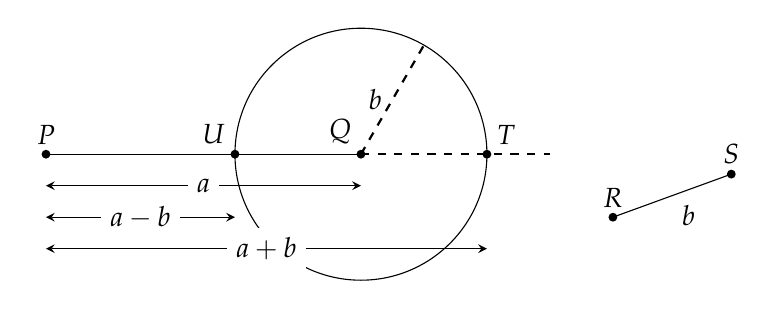
\begin{tikzpicture}[scale=.8]
\draw (0,0) -- (5,0);
\fill (0,0) node[above] {$P$} circle[radius=2pt];
\fill (5,0) node[above left] {$Q$} circle[radius=2pt];
\fill (3,0) node[above left] {$U$} circle[radius=2pt];
\fill (7,0) node[above right] {$T$} circle[radius=2pt];
\draw[thick,dashed] (5,0) -- (8,0);
\draw (5,0) circle[radius=2cm];
\draw[thick,dashed] (5,0) -- node[left] {$b$} ++(60:2cm);
\draw (9,-1) node[above] {$R$} -- node[below right] {$b$} ++(20:2cm) node[above] {$S$};
\fill (9,-1) circle[radius=2pt];
\fill (9,-1) ++(20:2cm) circle[radius=2pt];
\draw[<->] (0,-.5) -- node[fill=white] {$a$} (5,-.5);
\draw[<->] (0,-1) -- node[fill=white] {$a-b$} (3,-1);
\draw[<->] (0,-1.5) -- node[fill=white] {$a+b$} (7,-1.5);
\end{tikzpicture}
\end{center}

\newpage

\subsection*{Constructing an isosceles trapezoid}

Let $H$ be any point on $c(Q,b)$. Construct $H'$, its reflection about $\overline{PQ}$. $h$ is the length of $\overline{HH'}$:

\vspace{-1ex}

\begin{center}
\begin{tikzpicture}[scale=.6]
\coordinate (Q) at (0,0);
\coordinate (P) at (-6.8,0);
\coordinate (B) at (-3,-2);
\draw[thick,dashed] ($(Q)!1.3!(P)$) -- node[above,near start] {$a$} ($(P)!2.3!(Q)$);
\fill (Q) node[above left] {$Q$} circle[radius=2pt];
\fill (P) node[above] {$P$} circle[radius=2pt];
\fill (B) circle[radius=2pt];
\node[draw,circle through=(B),name path=qb] at (Q) {};
\draw[thick,dashed] (Q) -- node[left,xshift=-1pt,yshift=2pt] {$b$} (B);
\path[name path=qh] (Q) -- (-40:5cm);
\path[name path=qhp] (Q) -- (40:5cm);
\path [name intersections={of=qb and qh,by={H}}];
\path [name intersections={of=qb and qhp,by={Hp}}];
\fill[below right] (H) node[right,xshift=2pt] {$H$} circle[radius=2pt];
\fill[above right] (Hp) node[right,xshift=2pt] {$H'$} circle[radius=2pt];
\draw[thick,dashed] (H) -- node[below left,yshift=-2pt] {$h$} (Hp);
\end{tikzpicture}
\end{center}

\vspace{-2ex}

Construct the circles $c(H,b)$, $c(Q,h)$. Let $K$ be the intersection of the circles and construct $K'$, the reflection of $K$ about line $\overline{PQ}$:

\begin{center}
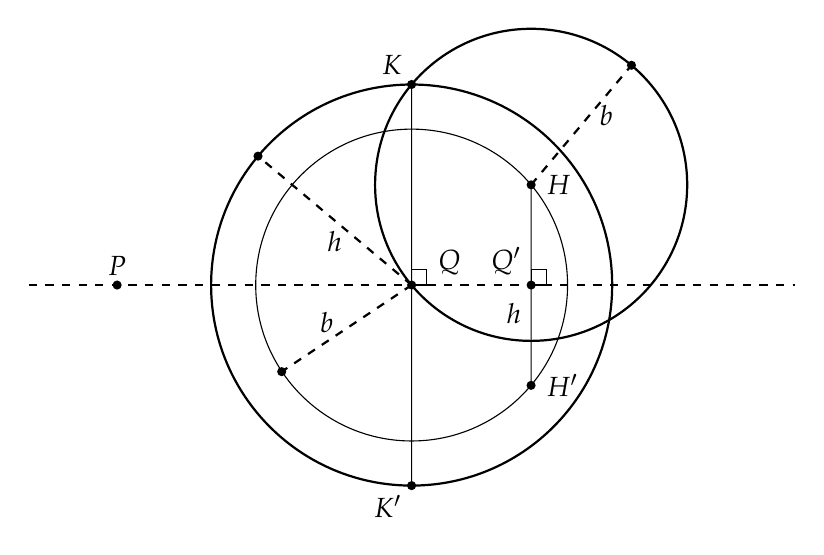
\begin{tikzpicture}[scale=.55]
\coordinate (Q) at (0,0);
\coordinate (P) at (-6.8,0);
\coordinate (B) at (-3,-2);
\draw[thick,dashed] ($(Q)!1.3!(P)$) -- ($(P)!2.3!(Q)$);
\fill (Q) node[above right,xshift=6pt] {$Q$} circle[radius=3pt];
\fill (P) node[above] {$P$} circle[radius=3pt];
\fill (B) circle[radius=3pt];
\node[draw,circle through=(B),name path=qb] at (Q) {};
\draw[thick,dashed] (Q) -- node[left,xshift=-1pt,yshift=2pt] {$b$} (B);
\path[name path=qh] (Q) -- (-40:5cm);
\path[name path=qhp] (Q) -- (40:5cm);
\path [name intersections={of=qb and qh,by={Hp}}];
\path [name intersections={of=qb and qhp,by={H}}];
\fill (H) node[right,xshift=2pt] {$H$} circle[radius=3pt];
\fill (Hp) node[right,xshift=2pt] {$H'$} circle[radius=3pt];
\draw (H) -- node[below left,yshift=-3pt] {$h$} (Hp);

\draw (H|-Q) rectangle +(10pt,10pt);
\fill (H|-Q) circle(3pt) node[above left] {$Q'$};

\draw[thick,name path=circleqh] (Q) let
  \p1 = ($ (H) - (Hp) $),
  \n2 = {veclen(\x1,\y1)}
in
  circle (\n2)
  (Q) edge [dashed] node[below] {$h$} +(140:\n2) ++(140:\n2) coordinate (q);
\fill (q) circle[radius=3pt];
\draw[thick,name path=circlehb] (H) let
  \p1 = ($ (Q) - (B) $),
  \n2 = {veclen(\x1,\y1)}
in
  circle (\n2)
  (H) edge [dashed] node[below,near end] {$b$} +(50:\n2) ++(50:\n2)  coordinate (h);
\fill (h) circle[radius=3pt];
\path [name intersections={of=circleqh and circlehb,by={K}}];
\fill (K) node[above left] {$K$} circle[radius=3pt];
%\draw[thick] (H) -- (K);
\draw let
  \p1 = ($ (K) - (Q) $)
in
  coordinate (Kp) at (\x1,-\y1);
\fill (Kp) node[below left] {$K'$} circle[radius=3pt];
\draw (K) -- (Kp);
\draw (Q) rectangle +(10pt,10pt);
\end{tikzpicture}
\vspace*{-8pt}
\end{center}

$\overline{PQ}$ is the perpendicular bisector of both $\overline{HH'}$ and $\overline{KK'}$, so these line segments are parallel. $\overline{KH}=b$ since it is the radius of the circle centered on $H$. $K',H'$ are reflections of $K,H$ and it is not hard to show that $\overline{K'H'}=\overline{KH}$ ($\triangle QQ'H\cong \triangle QQ'H'$ and then $\triangle KQH\cong \triangle K'QH'$). Therefore, $\overline{KHH'K'}$ is an isosceles trapezoid whose bases are $\overline{HH'}=h$, $\overline{KK'}=2h$. Let $d$ be the length of the diagonals $\overline{K'H}=\overline{KH'}$:


\begin{center}
\vspace*{-8pt}
\begin{tikzpicture}[scale=.6]
\coordinate (Q) at (0,0);
\coordinate (P) at (-6.8,0);
\coordinate (B) at (-3,-2);
\draw[thick,dashed] ($(Q)!1.3!(P)$) -- ($(P)!2.3!(Q)$);
\fill (Q) node[above left] {$Q$} circle[radius=3pt];
\fill (P) node[above] {$P$} circle[radius=3pt];
%\fill (B) circle[radius=3pt];
\node[draw,circle through=(B),name path=qb] at (Q) {};
%\draw[thick,dashed] (Q) -- node[left,xshift=-1pt,yshift=2pt] {$b$} (B);
\path[name path=qh] (Q) -- (-40:5cm);
\path[name path=qhp] (Q) -- (40:5cm);
\path [name intersections={of=qb and qh,by={Hp}}];
\path [name intersections={of=qb and qhp,by={H}}];
\fill (H) node[right,xshift=2pt] {$H$} circle[radius=3pt];
\fill (Hp) node[right,xshift=2pt] {$H'$} circle[radius=3pt];
\draw (H) -- node[below right,yshift=-2pt] {$h$} (Hp);
\path[name path=circleqh] (Q) let
  \p1 = ($ (H) - (Hp) $)
in
  circle ({veclen(\x1,\y1)});
\path[name path=circlehb] (H) let
  \p1 = ($ (Q) - (B) $)
in
  circle ({veclen(\x1,\y1)});
\path [name intersections={of=circleqh and circlehb,by={K,k2}}];
\fill (K) node[above left] {$K$} circle[radius=3pt];
\draw (Q) -- node[left] {$h$} (K);
\draw (H) -- node[right,xshift=4pt] {$b$} (K);
\draw let
  \p1 = ($ (K) - (Q) $)
in
  coordinate (Kp) at (\x1,-\y1);
\fill (Kp) node[below left] {$K'$} circle[radius=3pt];
\draw (Q) -- node[left] {$h$} (Kp) -- node[right,xshift=2pt,yshift=-2pt] {$b$} (Hp);
\draw (K) -- node[above right] {$d$} (Hp);
\draw (Kp) -- node[left] {$d$} (H);
\end{tikzpicture}
\label{ptolemy}
\vspace*{-8pt}
\end{center}

\subsection*{Circumscribing the trapezoid by a circle}

We want to proof that it is possible to circumscribe $\overline{KHH'K'}$ by a circle. We will prove that: if the opposite angles of a quadrilateral are supplementary, then the trapezoid can be circumscribed by a circle, and that in an isosceles trapezoid the opposite angles are supplementary. Geometry textbooks give the simple proof that the opposite angles of a quadrilateral circumscribed by a circle are supplementary, but it is hard to find a proof of the converse, so I present both proofs here.

\textbf{If a quadrilateral can be circumscribed by a circle then the opposite angles are supplementary:} An inscribed angle equals half the subtended arc, so $\angle DAB$ is half of the arc $\widehat{DCB}$ and $\angle DCB$ is half of the arc $\widehat{DAB}$. The two arcs subtend the entire circumference of the circle, so their sum is $360^\circ$. Therefore, $\angle DAB + \angle DCB = \disfrac{1}{2} \cdot 360^\circ =  180^\circ$, and similarly $\angle ADC + \angle ABC = 180^\circ$

\vspace*{-2ex}

\begin{center}
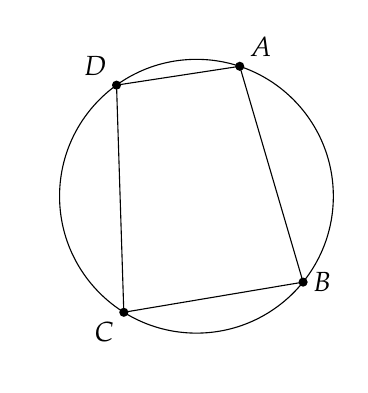
\begin{tikzpicture}[scale=.55]
\coordinate (origin) at (0,0);
\coordinate (A) at (1,3);
\node[draw,circle through=(A),name path=circle] at (origin) {};
\fill (A) node[above right] {$A$} circle[radius=3pt];
\path[name path=b] (A) -- (-50:4.5cm);
\path[name path=c] (A) -- (-120:4.5cm);
\path[name path=d] (A) -- (150:4.5cm);
\path [name intersections={of=circle and b,by={b1,B}}];
\fill (B) node[right] {$B$} circle[radius=3pt];
\path [name intersections={of=circle and c,by={c1,C}}];
\fill (C) node[below left] {$C$} circle[radius=3pt];
\path [name intersections={of=circle and d,by={d1,D}}];
\fill (D) node[above left] {$D$} circle[radius=3pt];
\draw (A) -- (B) -- (C) -- (D) -- cycle;
\end{tikzpicture}
\end{center}

\vspace*{-2ex}

\textbf{A quadrilateral whose opposite angles are supplementary can be circumscribed by a circle:} Any triangle can be circumscribed by a circle. Circumscribe $\triangle DAB$ by a circle and suppose that $C'$ is a point such that $\angle DAB + \angle DC'B = 180^\circ$, but $C'$ is \emph{not} on the circumference of the circle. Without loss of generality, let $C'$ be within the circle:

\vspace*{-1ex}

\begin{center}
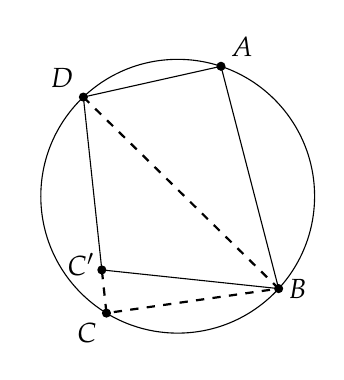
\begin{tikzpicture}[scale=.55]
\coordinate (origin) at (0,0);
\coordinate (A) at (1,3);
\node[draw,circle through=(A),name path=circle] at (origin) {};
\fill (A) node[above right] {$A$} circle[radius=3pt];
\path[name path=b] (A) -- (-50:4cm);
\path[name path=c] (A) -- (-120:4cm);
\path[name path=d] (A) -- (150:4cm);
\path [name intersections={of=circle and b,by={b1,B}}];
\fill (B) node[right] {$B$} circle[radius=3pt];
\path [name intersections={of=circle and c,by={c1,C}}];
\fill (C) node[below left] {$C$} circle[radius=3pt];
\path [name intersections={of=circle and d,by={d2,D}}];
\fill (D) node[above left] {$D$} circle[radius=3pt];
\coordinate (Cp) at ($(C)!.2!(D)$);
\draw (A) -- (B) -- (Cp) -- (D) -- cycle;
\fill (Cp) node[left,xshift=1pt,yshift=2pt] {$C'$} circle[radius=3pt];
\draw[thick,dashed] (D) -- (B) -- (C) -- (Cp);
\end{tikzpicture}
\end{center}

\vspace*{-1ex}

Construct a ray that extends $\overline{DC'}$ and let $C$ be its intersection with the circle. $\overline{ABCD}$ is circumscribed by a circle so:
\begin{eqnarray*}
\angle DAB + \angle DCB &=& 180^\circ\\
\angle DAB + \angle DCB &=& \angle DAB + \angle DC'B\\
\angle DCB &=& \angle DC'B\,,
\end{eqnarray*}
which is impossible if $C$ is on the circle and $C'$ is inside the circle.

\newpage

Finally, we show that the opposite angles of an isosceles trapezoid are supplementary.

\begin{center}
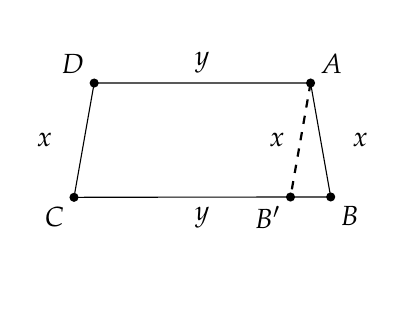
\begin{tikzpicture}[scale=.55]
\coordinate (origin) at (0,0);
\coordinate (A) at (2.5,1.8);
\node[circle through=(A),name path=circle] at (origin) {};
\fill (A) node[above right] {$A$} circle[radius=3pt];
\path[name path=b] (A) -- ++(-80:4cm);
\path[name path=d] (A) -- ++(180:6cm);
\path [name intersections={of=circle and b,by={b1,B}}];
\fill (B) node[below right] {$B$} circle[radius=3pt];
\path [name intersections={of=circle and d,by={d1,D}}];
\fill (D) node[above left] {$D$} circle[radius=3pt];
\path[name path=c] (D) -- ++(-100:4cm);
\path [name intersections={of=circle and c,by={c1,C}}];
\fill (C) node[below left] {$C$} circle[radius=3pt];
\draw (A) -- node[right,xshift=8pt] {$x$} (B);
\draw[name path=bc] (B) -- node[below] {$y$} (C);
\draw (C) -- node[left,xshift=-8pt] {$x$} (D) -- node[above] {$y$} (A);
\path[name path=para] (A) -- ++(-100:4cm);
\path [name intersections={of=para and bc,by={Bp}}];
\fill (Bp) node[below left] {$B'$} circle[radius=3pt];
\draw[thick,dashed] (A) -- node[left,xshift=-2pt] {$x$} (Bp);
\end{tikzpicture}
\end{center}

\vspace{-4ex}

Construct the line $\overline{AB'}$ parallel to $\overline{CD}$. $\overline{AB'CD}$ is a parallelogram and $\triangle ABB'$ is an isosceles triangle, so $\angle C= \angle ABB' = \angle AB'B = \angle B$. Similarly, $\angle A = \angle D$. Since the sum of the internal angles of any quadrilateral is equal to $360^\circ$:
\begin{eqnarray*}
\angle A + \angle B + \angle C + \angle D &=& 360^\circ\\
2\angle A + 2 \angle C &=& 360^\circ\\
\angle A +  \angle C &=& 180^\circ\,.
\end{eqnarray*}
and similarly $\angle B +  \angle D = 180^\circ$.

\subsection*{Ptolemy's theorem}

Ptolemy's theorem relates the lengths of the diagonals and the lengths of the sides of a quadrilateral that is circumscribed by a circle:
\[
ef = ac + bd\,.
\]
\begin{center}
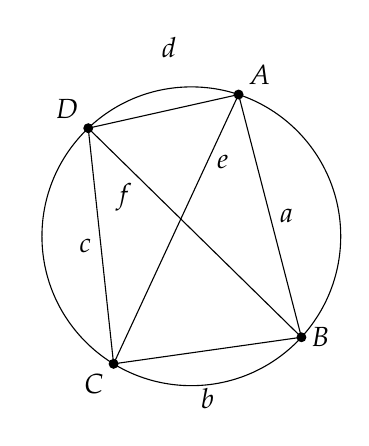
\begin{tikzpicture}[scale=.6]
\coordinate (origin) at (0,0);
\coordinate (A) at (1,3);
\node[draw,circle through=(A),name path=circle] at (origin) {};
\fill (A) node[above right] {$A$} circle[radius=3pt];
\path[name path=b] (A) -- (-50:4cm);
\path[name path=c] (A) -- (-120:4cm);
\path[name path=d] (A) -- (150:4cm);
\path [name intersections={of=circle and b,by={b1,B}}];
\fill (B) node[right] {$B$} circle[radius=3pt];
\path [name intersections={of=circle and c,by={C,c2}}];
\fill (C) node[below left] {$C$} circle[radius=3pt];
\path [name intersections={of=circle and d,by={D,d2}}];
\fill (D) node[above left] {$D$} circle[radius=3pt];
\draw (A) -- node[right] {$a$} (B) -- node[below,yshift=-10pt] {$b$} (C) -- node[left] {$c$} (D) -- node[above,xshift=2pt,yshift=16pt] {$d$}  cycle;
\draw (A) -- node[right,near start] {$e$} (C);
\draw (B) -- node[left,near end,yshift=-6pt] {$f$} (D);
\end{tikzpicture}
\end{center}
There is a geometric proof of the theorem (see Wikipedia), but I will present a simple trigonometric proof. The law of cosines for the four triangles $\triangle ABC$, $\triangle ADC$, $\triangle DAB$, $\triangle DCB$ gives the following equations:
\begin{eqnarray*}
e^2 &=& a^2 + b^2 - 2ab \cos \angle B\\
e^2 &=& c^2 + d^2 - 2cd \cos \angle D\\
f^2 &=& a^2 + d^2 - 2ad \cos \angle A\\
f^2 &=& b^2 + c^2 - 2bc \cos \angle C\,.
\end{eqnarray*}
$\angle C = 180^\circ - \angle A$ and $\angle D = 180^\circ - \angle B$ because they are opposite angles of a quadrilateral circumscribed by a circle, so:
\begin{eqnarray*}
\cos \angle D &=& - \cos \angle B\\
\cos \angle C &=& -\cos \angle A\,.
\end{eqnarray*}
We can eliminate the cosine term from the first two equations and from the last two equations. After some messy arithmetic, we get:
\begin{eqnarray*}
e^2 &=& \frac{(ac+bd)(ad+bc)}{(ab+cd)}\\
f^2 &=& \frac{(ab+cd)(ac+bd)}{(ad+bc)}\,.
\end{eqnarray*}
Multiply the two equations and simplify to get Ptolemy's theorem:
\begin{eqnarray*}
e^2\cdot f^2 &=& (ac+bd)^2\\
ef &=& (ac+bd)\,. 
\end{eqnarray*}
\subsection*{Using Ptolemy's theorem}

For the construction on page~\pageref{ptolemy}, the diagonals are of length $d$, the legs are of length $b$, and the bases are of lengths $h$ and $2h$, so Ptolemy's theorem gives $d\cdot d = b\cdot b + h\cdot 2h$ or $d^2=b^2+2h^2$.

Let $X$ be the point on line $\overline{PQ}$ that extends $\overline{PQ}$ by $b$. (We will eventually construct $X$; now we're just imagining it.) Define  $x = \overline{K'X}$. Since $\triangle QK'X$ is a right triangle, $x^2 = b^2 + h^2$:
\begin{center}
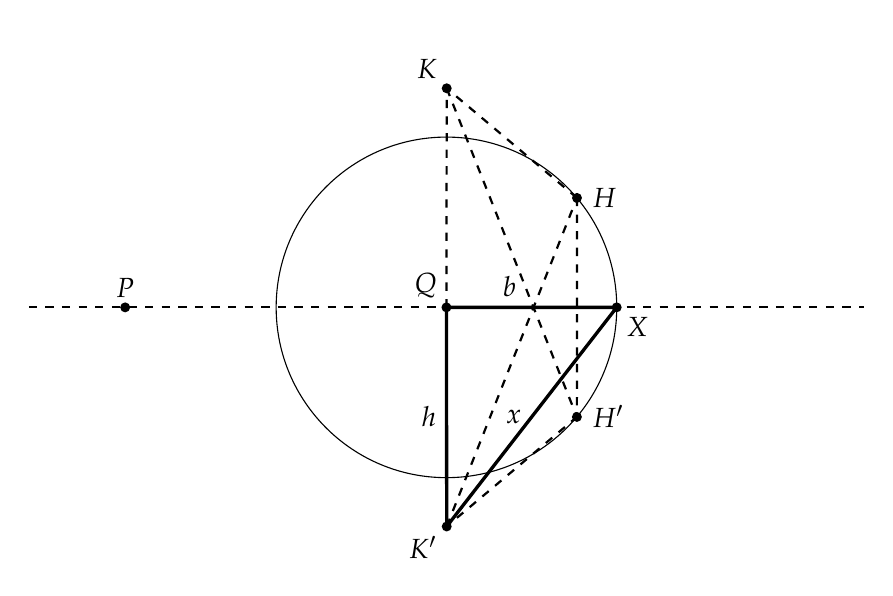
\begin{tikzpicture}[scale=.6]
\coordinate (Q) at (0,0);
\coordinate (P) at (-6.8,0);
\coordinate (B) at (-3,-2);
\draw[thick,dashed,name path=pq] ($(Q)!1.3!(P)$) -- ($(P)!2.3!(Q)$);
\fill (Q) node[above left] {$Q$} circle[radius=3pt];
\fill (P) node[above] {$P$} circle[radius=3pt];
%\fill (B) circle[radius=2pt];
\node[draw,circle through=(B),name path=qb] at (Q) {};
%\draw[thick,dashed] (Q) -- node[left,xshift=-1pt,yshift=2pt] {$b$} (B);
\path[name path=qh] (Q) -- (-40:5cm);
\path[name path=qhp] (Q) -- (40:5cm);
\path [name intersections={of=qb and qh,by={hp}}];
\path [name intersections={of=qb and qhp,by={H}}];
\fill (H) node[right,xshift=2pt] {$H$} circle[radius=3pt];
\fill (hp) node[right,xshift=2pt] {$H'$} circle[radius=3pt];
\draw[thick,dashed] (H) -- (hp);
\path[name path=circleqh] (Q) let
  \p1 = ($ (H) - (hp) $)
in
  circle ({veclen(\x1,\y1)});
\path[name path=circlehb] (H) let
  \p1 = ($ (Q) - (B) $)
in
  circle ({veclen(\x1,\y1)});
\path [name intersections={of=circleqh and circlehb,by={K,k2}}];
\fill (K) node[above left] {$K$} circle[radius=3pt];
\draw[thick,dashed] (Q) -- (K);
\draw[thick,dashed] (H) -- (K);
\draw[thick,dashed] let
  \p1 = ($ (K) - (Q) $)
in
  coordinate (kp) at (\x1,-\y1);
\fill (kp) node[below left] {$K'$} circle[radius=3pt];
\draw[thick,dashed] (Q) -- node[left] {$h$} (kp) -- (hp);
\draw[thick,dashed] (K) -- (hp);
\draw[thick,dashed] (kp) -- (H);
\path [name intersections={of=pq and qb,by={X,x2}}];
\fill (X) node[below right] {$X$} circle[radius=3pt];
\draw[thick,dashed] (kp) -- node[left] {$x$} (X);
\draw[very thick] (Q) -- (kp) -- (X) -- node[above,xshift=-8pt] {$b$} cycle;
\end{tikzpicture}
\vspace*{-8pt}
\end{center}
From the computation of Ptolemy's theorem theorem above:
\erh{0pt}
\begin{equationarray*}{rcl}
d^2&=&b^2 + 2h^2\\
&=&(x^2-h^2)+2h^2\\
&=&x^2+h^2\,.
\end{equationarray*}
Don't look for a right triangle in the diagram. We are claiming that \emph{it is possible to construct} a triangle with sides $x,h,d$. 

Let us construct the point $S$ as the intersection of the circles 
$c(K,d),c(K',d)$:
\begin{center}
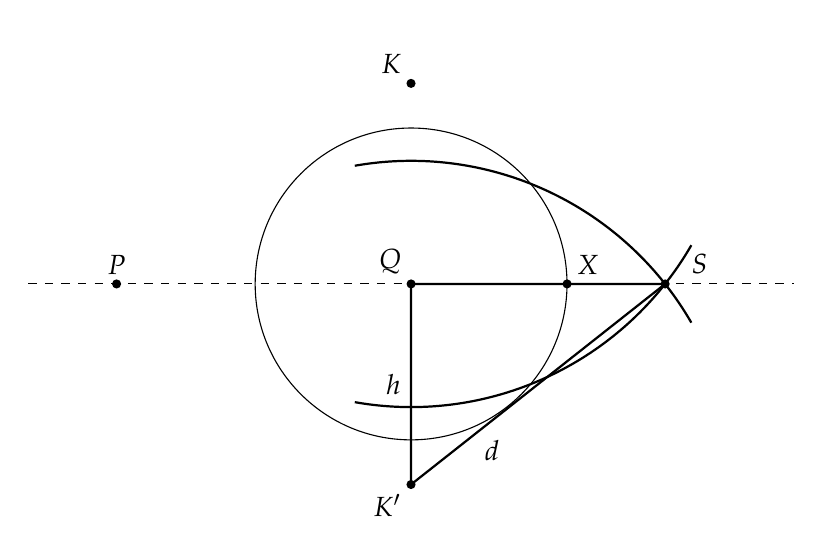
\begin{tikzpicture}[scale=.55]
\coordinate (Q) at (0,0);
\coordinate (P) at (-6.8,0);
\coordinate (B) at (-3,-2);
\draw[dashed,name path=pq] ($(Q)!1.3!(P)$) -- ($(P)!2.3!(Q)$);
\fill (Q) node[above left] {$Q$} circle[radius=3pt];
\fill (P) node[above] {$P$} circle[radius=3pt];
\node[draw,circle through=(B),name path=qb] at (Q) {};
\path[name path=qh] (Q) -- (-40:5cm);
\path[name path=qhp] (Q) -- (40:5cm);
\path [name intersections={of=qb and qh,by={Hp}}];
\path [name intersections={of=qb and qhp,by={H}}];
%\fill (H) node[right,xshift=2pt] {$H$} circle[radius=3pt];
%\fill (Hp) node[right,xshift=2pt] {$H'$} circle[radius=3pt];
\path[name path=circleqh] (Q) let
  \p1 = ($ (H) - (Hp) $)
in
  circle ({veclen(\x1,\y1)});
\path[name path=circlehb] (H) let
  \p1 = ($ (Q) - (B) $)
in
  circle ({veclen(\x1,\y1)});
\path [name intersections={of=circleqh and circlehb,by={K,k2}}];
\fill (K) node[above left] {$K$} circle[radius=3pt];
\draw[thick,dashed] let
  \p1 = ($ (K) - (Q) $)
in
  coordinate (Kp) at (\x1,-\y1);
\fill (Kp) node[below left] {$K'$} circle[radius=3pt];
\draw[thick] (Q) -- node[left] {$h$} (Kp);
\draw[thick,name path=khp] (K) let
  \p1 = ($ (H) - (Kp) $),
  \n2 = {veclen(\x1,\y1)}
in
  (K) ++(-100:\n2) arc (-100:-30:\n2);
\draw[thick,name path=kph] (Kp) let
  \p1 = ($ (H) - (Kp) $),
  \n2 = {veclen(\x1,\y1)}
in
  (Kp) ++(100:\n2) arc (100:30:\n2);
\path [name intersections={of=kph and khp,by={S}}];
\fill (S) node[above right,xshift=6pt] {$S$} circle[radius=3pt];
\draw[thick] (Kp) -- node[right,near start,yshift=-6pt] {$d$} (S);
\draw[thick] (Q) -- (S);
\path [name intersections={of=pq and qb,by={X,Xp}}];
\fill (X) node[above right] {$X$} circle[radius=3pt];
%\fill (Xp) node[above left] {$X'$} circle[radius=3pt];
%\draw (Kp) -- node[left] {$x$} (X);
%\draw (K) -- node[left] {$x$} (X);
%\fill (B) circle[radius=3pt];
%\draw[thick,dashed] (Q) -- node[left,xshift=-1pt,yshift=2pt] {$b$} (B);
\end{tikzpicture}
\end{center}
We obtain a right triangle $\triangle QSK'$. By Pythagoras' theorem 
$\overline{QS}^2 + h^2 = d^2$, so:
\[
\overline{QS}^2 = d^2-h^2=x^2\,,
\]
and $\overline{QS}=x$.

It is possible to construct the point $X$ as the intersection of the circles $c(K,x),c(K',x)$:
\begin{center}
\vspace*{-14pt}
\begin{tikzpicture}[scale=.55]
\coordinate (Q) at (0,0);
\coordinate (P) at (-6.8,0);
\coordinate (B) at (-3,-2);
\draw[dashed,name path=pq] ($(Q)!1.3!(P)$) -- ($(P)!2.3!(Q)$);
\fill (Q) node[above left] {$Q$} circle[radius=3pt];
\fill (P) node[above] {$P$} circle[radius=3pt];
\node[draw,circle through=(B),name path=qb] at (Q) {};
\path[name path=qh] (Q) -- (-40:5cm);
\path[name path=qhp] (Q) -- (40:5cm);
\path [name intersections={of=qb and qh,by={Hp}}];
\path [name intersections={of=qb and qhp,by={H}}];
%\fill (H) node[right,xshift=2pt] {$H$} circle[radius=3pt];
%\fill (Hp) node[right,xshift=2pt] {$H'$} circle[radius=3pt];
\path[name path=circleqh] (Q) let
  \p1 = ($ (H) - (Hp) $)
in
  circle ({veclen(\x1,\y1)});
\path[name path=circlehb] (H) let
  \p1 = ($ (Q) - (B) $)
in
  circle ({veclen(\x1,\y1)});
\path [name intersections={of=circleqh and circlehb,by={K,k2}}];
\fill (K) node[above left] {$K$} circle[radius=3pt];
\path[thick,dashed] let
  \p1 = ($ (K) - (Q) $)
in
  coordinate (Kp) at (\x1,-\y1);
\fill (Kp) node[below left] {$K'$} circle[radius=3pt];
%\draw[thick] (Q) -- node[left] {$h$} (Kp);
\path[name path=khp] (K) let
  \p1 = ($ (H) - (Kp) $),
  \n2 = {veclen(\x1,\y1)}
in
  (K) ++(-100:\n2) arc (-100:-30:\n2);
\path[name path=kph] (Kp) let
  \p1 = ($ (H) - (Kp) $),
  \n2 = {veclen(\x1,\y1)}
in
  (Kp) ++(100:\n2) arc (100:30:\n2);
\path [name intersections={of=kph and khp,by={S}}];
\fill (S) node[above right,xshift=6pt] {$S$} circle[radius=3pt];
%\draw[thick] (Kp) -- node[right,near start,yshift=-6pt] {$d$} (S);
%\draw[thick] (Q) -- (S);
\path [name intersections={of=pq and qb,by={X,Xp}}];
\fill (X) node[above right,xshift=8pt] {$X$} circle[radius=3pt];
\fill (Xp) node[above left] {$X'$} circle[radius=3pt];
\draw (Kp) -- node[left] {$x$} (X);
\draw (K) -- node[left] {$x$} (X);
%\fill (B) circle[radius=3pt];
%\draw[thick,dashed] (Q) -- node[left,xshift=-1pt,yshift=2pt] {$b$} (B);
\draw[name path=kx] (K) let
  \p1 = ($ (X) - (Kp) $),
  \n2 = {veclen(\x1,\y1)}
in
  (K) ++(-100:\n2) arc (-100:-30:\n2);
\draw[name path=kpx] (Kp) let
  \p1 = ($ (X) - (Kp) $),
  \n2 = {veclen(\x1,\y1)}
in
  (Kp) ++(100:\n2) arc (100:30:\n2);
\path (Xp) -- node[below] {$b$} (Q);
\path (Q) -- node[below] {$b$} (X);
\node at (-5,2) {\mbox{\boldmath $\overline{PQ}=a$}};
\draw[thick,dashed] (Q) -- node[left] {$h$} (Kp);
\draw[thick,dashed] (Q) -- (X);
\end{tikzpicture}
\vspace*{-10pt}
\end{center}
Recall that we want to extend $\overline{PQ}$ of length $a$ by a length $b$, or decrease its length by $b$. Since the length of $\overline{QX}$ is $\sqrt{x^2-h^2}=b$, the length of $\overline{PX}$ is $a+b$ and the length of $\overline{PX'}$ is $a-b$.

%%%%%%%%%%%%%%%%%%%%%%%%%%%%%%%%%%%%%%%%%%%%%%%%%%%%%%%%%%%%%%%

\section{Construct a line segment relative to three other line segments}\label{s.three}

\textbf{Given line segments of length $n,m,s$, construct a line segment of length:}
\[
x = \disfrac{n}{m}s\,.
\]

Construct two concentric circles $c_1 = c(Z,m)$ and $c_2 = c(Z,n)$, and chord $\overline{AB} = s$ on $c_1$. (A chord can be constructed using only a compass as shown in Section~\ref{s.circle}.)

We assume that $m>n$. If not, exchange the notation.
\begin{center}
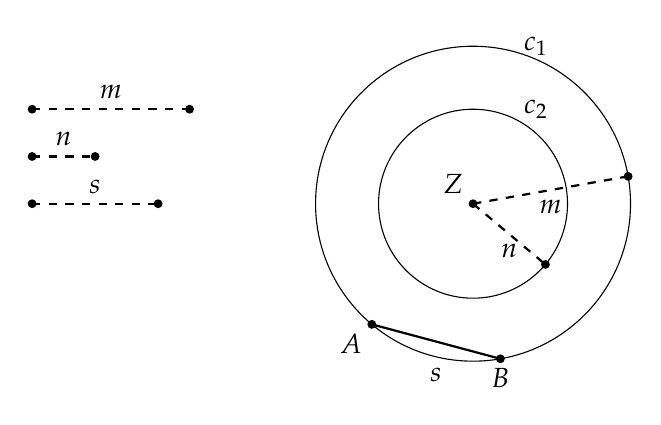
\begin{tikzpicture}[scale=.4]
\coordinate (Z) at (0,0);
\coordinate (A) at (-130:5cm);
\coordinate (B) at (-80:5cm);
\fill (Z) node[above left] {$Z$} circle[radius=4pt];
\fill (A) node[below left] {$A$} circle[radius=4pt];
\fill (B) node[below] {$B$} circle[radius=4pt];
\draw[name path=c1] (Z) circle[radius=5cm];
\draw[name path=c2] (Z) circle[radius=3cm];
\node at (2,5) {$c_1$};
\node at (2,3) {$c_2$};
\draw[thick] (A) -- node[below,yshift=-6pt] {$s$} (B);
\draw[thick,dashed] (Z) -- node[below] {$m$} ++(10:5cm);
\draw[thick,dashed] (Z) -- node[below] {$n$} ++(-40:3cm);
\fill (Z) ++ (10:5cm) circle[radius=4pt];
\fill (Z) ++ (-40:3cm) circle[radius=4pt];
\begin{scope}[xshift=-14cm,yshift=3cm]
\coordinate (m) at (0,0);
\coordinate (n) at (0,-1.5);
\coordinate (s) at (0,-3);
\coordinate (mp) at (5,0);
\coordinate (np) at (2,-1.5);
\coordinate (sp) at (4,-3);
\fill (m) circle[radius=4pt];
\fill (n) circle[radius=4pt];
\fill (s) circle[radius=4pt];
\fill (mp) circle[radius=4pt];
\fill (np) circle[radius=4pt];
\fill (sp) circle[radius=4pt];
\draw[thick,dashed] (m) -- node[above] {$m$} (mp);
\draw[thick,dashed] (n) -- node[above] {$n$} (np);
\draw[thick,dashed] (s) -- node[above] {$s$} (sp);
\end{scope}
\end{tikzpicture}
\end{center}

\vspace{-2ex}

We also assume that $s$ does not intersect $c_2$. If not, use the construction in Section~\ref{s.add-subtract} to multiply $m,n$ by a number $k$ so that the chord does not intersect the circle. Note that this does not change the value that we are trying to construct since $x=\disfrac{kn}{km}s=\disfrac{n}{m}s$.

Choose any point $H$ on circle $c_2$. Label the length of $\overline{AH}$ by $w$. Construct point $K$ on $c_2$ such that the length of $\overline{BK}$ is $w$.
\begin{center}
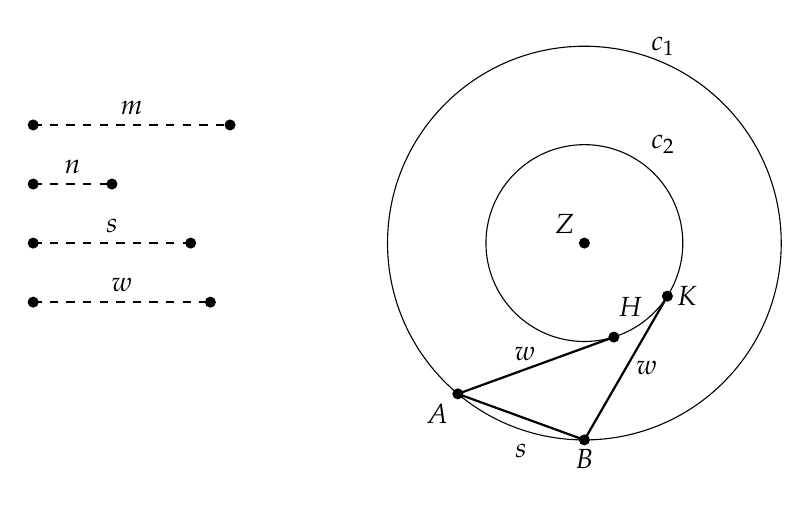
\begin{tikzpicture}[scale=.5]
\coordinate (Z) at (0,0);
\coordinate (A) at (-130:5cm);
\coordinate (B) at (-90:5cm);
\fill (Z) node[above left] {$Z$} circle[radius=4pt];
\fill (A) node[below left] {$A$} circle[radius=4pt];
\fill (B) node[below] {$B$} circle[radius=4pt];
\draw[name path=c1] (Z) circle[radius=5cm];
\draw[name path=c2] (Z) circle[radius=2.5cm];
\node at (2,5) {$c_1$};
\node at (2,2.5) {$c_2$};
\draw[thick] (A) -- node[below,yshift=-6pt] {$s$} (B);
\draw[thick] (A) -- node[above,xshift=-4pt,yshift=-2pt] {$w$} +(20:120pt) coordinate (H);
\fill (H) node[above right,xshift=-2pt,yshift=4pt] {$H$} circle[radius=4pt];
\draw[thick] (B) -- node[right] {$w$} +(60:120pt) coordinate (K);
\fill (K) node[right] {$K$} circle[radius=4pt];
\begin{scope}[xshift=-14cm,yshift=3cm]
\coordinate (m) at (0,0);
\coordinate (n) at (0,-1.5);
\coordinate (s) at (0,-3);
\coordinate (w) at (0,-4.5);
\coordinate (mp) at (5,0);
\coordinate (np) at (2,-1.5);
\coordinate (sp) at (4,-3);
\coordinate (wp) at (4.5,-4.5);
\fill (m) circle[radius=4pt];
\fill (n) circle[radius=4pt];
\fill (s) circle[radius=4pt];
\fill (w) circle[radius=4pt];
\fill (mp) circle[radius=4pt];
\fill (np) circle[radius=4pt];
\fill (sp) circle[radius=4pt];
\fill (wp) circle[radius=4pt];
\draw[thick,dashed] (m) -- node[above] {$m$} (mp);
\draw[thick,dashed] (n) -- node[above] {$n$} (np);
\draw[thick,dashed] (s) -- node[above] {$s$} (sp);
\draw[thick,dashed] (w) -- node[above] {$w$} (wp);
\end{scope}
\end{tikzpicture}
\end{center}

$\triangle AHZ\cong\triangle BZK$ by side-side-side: $\overline{ZA}=\overline{ZB}=m$, the radius of $c_1$, $\overline{ZH}=\overline{ZK}=n$, the radius of $c_2$, and $\overline{AH}=\overline{BK}=w$ by construction.

\begin{center}
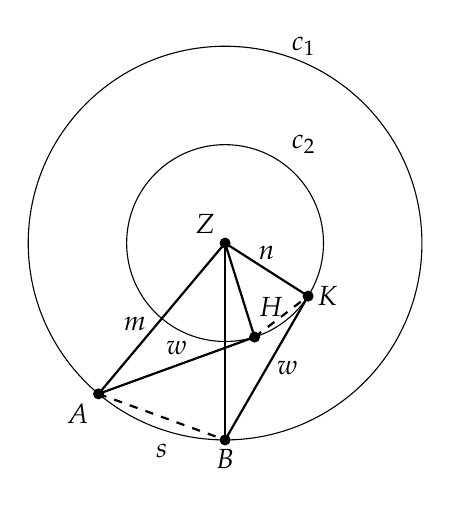
\begin{tikzpicture}[scale=.5]
\coordinate (Z) at (0,0);
\coordinate (A) at (-130:5cm);
\coordinate (B) at (-90:5cm);
\fill (Z) node[above left] {$Z$} circle[radius=4pt];
\fill (A) node[below left] {$A$} circle[radius=4pt];
\fill (B) node[below] {$B$} circle[radius=4pt];
\draw[name path=c1] (Z) circle[radius=5cm];
\draw[name path=c2] (Z) circle[radius=2.5cm];
\node at (2,5) {$c_1$};
\node at (2,2.5) {$c_2$};
\draw[thick,dashed] (A) -- node[below,yshift=-6pt] {$s$} (B);
\draw[thick] (A) -- node[above] {$w$} +(20:120pt) coordinate (H);
\fill (H) node[above right,xshift=-2pt,yshift=4pt] {$H$} circle[radius=4pt];
\draw[thick] (B) -- node[right] {$w$} +(60:120pt) coordinate (K);
\fill (K) node[right] {$K$} circle[radius=4pt];
\draw[thick] (Z) -- node[left,xshift=-2pt,yshift=-2pt] {$m$} (A);
\draw[thick] (Z) -- (B);
\draw[thick] (Z) -- (H);
\draw[thick] (Z) -- node[above] {$n$} (K);
\draw[thick,dashed] (H) -- (K);
\end{tikzpicture}
\end{center}
From $\triangle AHZ\cong\triangle BZK$, we get $\angle AZB = \angle HZK$. It is difficult to see this equality from the diagram, but the following diagram clarifies the relation among the angles. Define $\alpha = \angle AZH = \angle BZK$ and $\beta = \angle BZH$. It is easy to see that $\angle AZB = \angle HZK = \alpha - \beta$.
\begin{center}
\vspace*{-10pt}
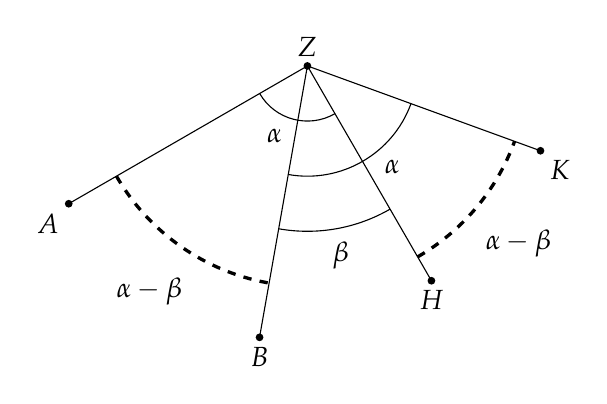
\begin{tikzpicture}[scale=.7]
\coordinate (Z) at (0,0);
\coordinate (A) at (-150:5cm);
\coordinate (B) at (-100:5cm);
\coordinate (H) at (-60:4.5cm);
\coordinate (K) at (-20:4.5cm);
\fill (Z) circle[radius=2pt];
\fill (A) circle[radius=2pt];
\fill (B) circle[radius=2pt];
\fill (H) circle[radius=2pt];
\fill (K) circle[radius=2pt];
\draw (A) node[below left] {$A$} -- (Z) node[above] {$Z$} -- (B) node[below] {$B$};
\draw (H) node[below] {$H$} -- (Z) -- (K) node[below right] {$K$};
\draw (-150:1cm) arc (-150:-60:1);
\draw (-100:2cm) arc (-100:-20:2);
\draw (-100:3cm) arc (-100:-60:3);
\draw[very thick,dashed] (-150:4cm) arc (-150:-100:4);
\draw[very thick,dashed] (-60:4cm) arc (-60:-20:4);
\node at (-115:1.4) {$\alpha$};
\node at (-50:2.4) {$\alpha$};
\node at (-80:3.5) {$\beta$};
\node at (-40:5) {$\alpha - \beta$};
\node at (-125:5) {$\alpha - \beta$};
\end{tikzpicture}
\vspace*{-10pt}
\end{center}

$\triangle ZAB\sim\triangle ZHK$ by side-angle-side, since both are isosceles triangles and we have shown that they have the same vertex angle.

\vspace{-2ex}

\begin{center}
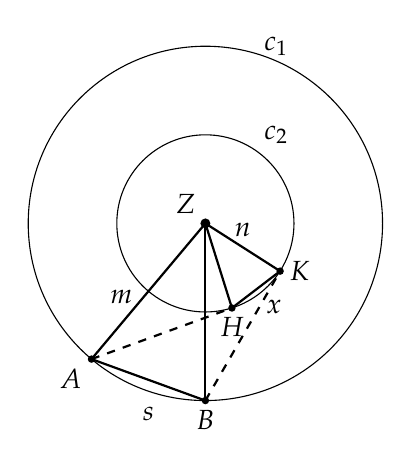
\begin{tikzpicture}[scale=.45]
\coordinate (Z) at (0,0);
\coordinate (A) at (-130:5cm);
\coordinate (B) at (-90:5cm);
\fill (Z) node[above left] {$Z$} circle[radius=4pt];
\fill (A) node[below left] {$A$} circle[radius=3pt];
\fill (B) node[below] {$B$} circle[radius=3pt];
\draw[name path=c1] (Z) circle[radius=5cm];
\draw[name path=c2] (Z) circle[radius=2.5cm];
\node at (2,5) {$c_1$};
\node at (2,2.5) {$c_2$};
\draw[thick] (A) -- node[below,yshift=-6pt] {$s$} (B);
\path[thick,dashed] (A) -- +(20:120pt) coordinate (H);
\fill (H) node[below] {$H$} circle[radius=3pt];
\path[thick,dashed] (B) -- +(60:120pt) coordinate (K);
\fill (K) node[right] {$K$} circle[radius=3pt];
\draw[thick] (Z) -- node[left,xshift=-2pt,yshift=-2pt] {$m$} (A);
\draw[thick] (Z) -- (B);
\draw[thick] (Z) -- (H);
\draw[thick] (Z) -- node[above] {$n$} (K);
\draw[thick] (H) -- node[below right] {$x$} (K);
\draw[thick,dashed] (A) -- (H);
\draw[thick,dashed] (B) -- (K);
\end{tikzpicture}
\end{center}

\vspace{-2ex}

Label $\overline{HK}$ by $x$. Then:

\vspace{-2ex}

\erh{10pt}
\begin{equationarray*}{rcl}
\frac{m}{s} &=& \frac{n}{x}\\
x&=&\frac{n}{m}s\,.
\end{equationarray*}

%%%%%%%%%%%%%%%%%%%%%%%%%%%%%%%%%%%%%%%%%%%%%%%%%%%%%%%%%%%%%%%

\vspace{-2ex}


\section{Find the intersection of two lines}\label{s.two-lines}

\textbf{Given two lines containing the line segments $\overline{AB}, \overline{CD}$, it is possible to construct their intersection using only a compass.}

Let $C',D'$ be the reflections of $C,D$ around $\overline{AB}$. $S$, the point of intersection of $\overline{CD}$ and $\overline{C'D'}$, lies on $\overline{AB}$, because $\triangle CZS\cong \triangle C'ZS$ by side-angle-side: $\overline{CZ}=\overline{C'Z}$, $\angle CZS=\angle C'ZS$ are right triangles and $\overline{ZS}$ is a common side. Therefore, $\overline{C'S}=\overline{CS}$ and similarly $\overline{D'S}=\overline{DS}$.


\begin{center}
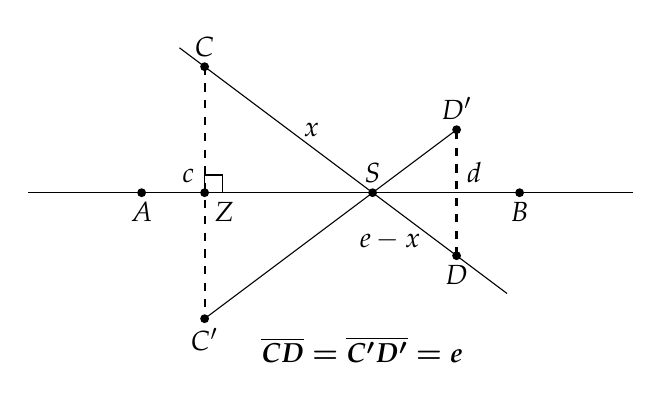
\begin{tikzpicture}[scale=.8]
\coordinate (A) at (-4,0);
\coordinate (B) at (2,0);
\coordinate (C) at (-3,2);
\coordinate (D) at (1,-1);
\coordinate (Cp) at (-3,-2);
\coordinate (Dp) at (1,1);
\fill (A) node[below] {$A$} circle[radius=2pt];
\fill (B) node[below] {$B$} circle[radius=2pt];
\fill (C) node[above] {$C$} circle[radius=2pt];
\fill (D) node[below] {$D$} circle[radius=2pt];
\fill (Cp) node[below] {$C'$} circle[radius=2pt];
\fill (Dp) node[above] {$D'$} circle[radius=2pt];
\draw[name path=ab] ($(A)!1.3!(B)$) -- ($(B)!1.3!(A)$);
\draw[name path=cd] ($(C)!1.2!(D)$) -- ($(D)!1.1!(C)$);
\path [name intersections={of=ab and cd,by={S}}];
\fill (S) node[above] {$S$} circle[radius=2pt];
\draw (Cp) -- (Dp);
\draw[thick,dashed] (C) -- node[above left] {$c$} (Cp);
\draw[thick,dashed] (D) -- node[above right] {$d$} (Dp);
\path (C) -- node[right,xshift=2pt] {$x$} (S);
\path (S) -- node[left,near end,xshift=-2pt] {$e-x$} (D);
\node at (-.5,-2.5) {\mbox{\boldmath $\overline{CD}=\overline{C'D'}=e$}};
\fill (C|-A)  node[below right] {$Z$} circle[radius=2pt];
\draw (C|-A) rectangle +(8pt,8pt);
\end{tikzpicture}
\end{center}

Label $x=\overline{CS}, c=\overline{CC'}, d=\overline{DD'},e=\overline{CD}$. $\triangle CSC'\sim\triangle DSD'$ are similar so $\disfrac{x}{e-x} = \frac{c}{d}$. Solving the equation for $x$ gives $x=\disfrac{c}{c+d}e$.

If $C,D$ are on the same side of $\overline{AB}$:
\begin{center}
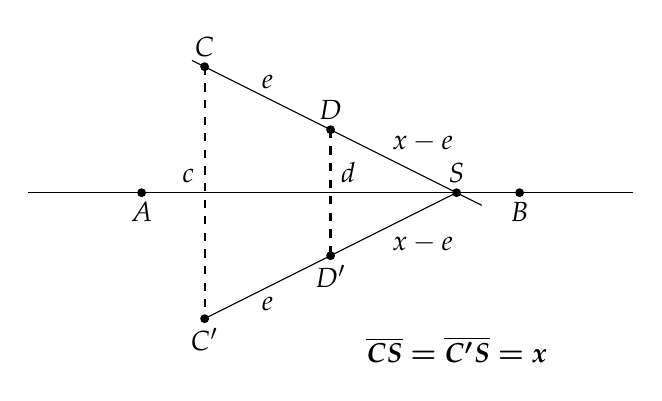
\begin{tikzpicture}[scale=.8]
\coordinate (A) at (-4,0);
\coordinate (B) at (2,0);
\coordinate (C) at (-3,2);
\coordinate (D) at (-1,1);
\coordinate (Cp) at (-3,-2);
\coordinate (Dp) at (-1,-1);
\fill (A) node[below] {$A$} circle[radius=2pt];
\fill (B) node[below] {$B$} circle[radius=2pt];
\fill (C) node[above] {$C$} circle[radius=2pt];
\fill (D) node[above] {$D$} circle[radius=2pt];
\fill (Cp) node[below] {$C'$} circle[radius=2pt];
\fill (Dp) node[below] {$D'$} circle[radius=2pt];
\draw[name path=ab] ($(A)!1.3!(B)$) -- ($(B)!1.3!(A)$);
\draw[name path=cd] ($(C)!2.2!(D)$) -- ($(D)!1.1!(C)$);
\path [name intersections={of=ab and cd,by={S}}];
\fill (S) node[above] {$S$} circle[radius=2pt];
\draw (Cp) -- (S);
\draw[thick,dashed] (C) -- node[above left] {$c$} (Cp);
\draw[thick,dashed] (D) -- node[above right] {$d$} (Dp);
\path (C) -- node[above] {$e$} (D);
\path (Cp) -- node[below] {$e$} (Dp);
\path (D) -- node[above right,xshift=-4pt] {$x-e$} (S);
\path (Dp) -- node[below right,xshift=-4pt] {$x-e$} (S);
\node at (1,-2.5) {\mbox{\boldmath $\overline{CS}=\overline{C'S}=x$}};
\end{tikzpicture}
\end{center}
$\triangle CSC'\sim\triangle DSD'$ gives $\disfrac{x}{x-e}=\disfrac{c}{d}$. Solving for $x$ gives $x=\disfrac{c}{c-d}e$.

\medskip

Construct the circles $c(C',d), c(D,e)$ and label their intersection by $H$. The sum of the line segments $\overline{CC'}, \overline{C'H}$ is $c + d$. We have to show that $H$ is on the extension of $\overline{CC'}$ so that $\overline{CH}$ is a line segment of length $c+d$. ($\overline{CH} = c - d$ in case $D$ is on the same side of $\overline{AB}$ as $C$.) 

\begin{center}
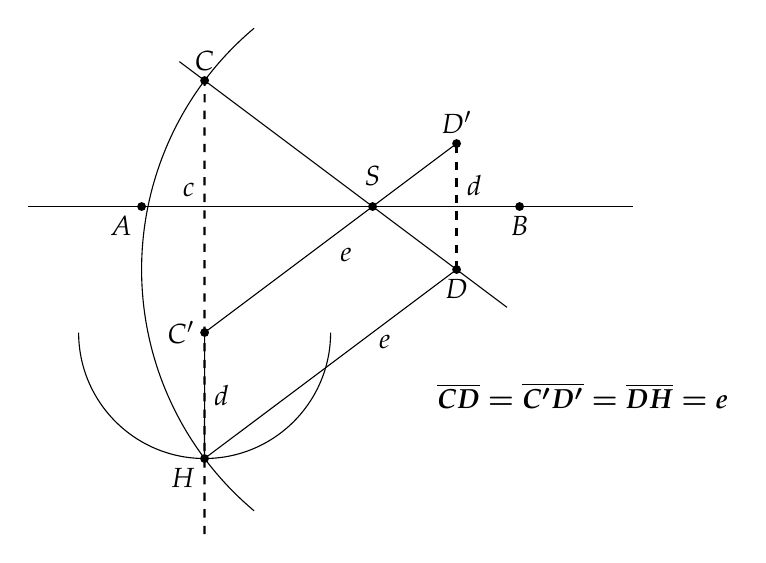
\begin{tikzpicture}[scale=.8]
\coordinate (A) at (-4,0);
\coordinate (B) at (2,0);
\coordinate (C) at (-3,2);
\coordinate (D) at (1,-1);
\coordinate (Cp) at (-3,-2);
\coordinate (Dp) at (1,1);
\fill (A) node[below left] {$A$} circle[radius=2pt];
\fill (B) node[below] {$B$} circle[radius=2pt];
\fill (C) node[above] {$C$} circle[radius=2pt];
\fill (D) node[below] {$D$} circle[radius=2pt];
\fill (Cp) node[left] {$C'$} circle[radius=2pt];
\fill (Dp) node[above] {$D'$} circle[radius=2pt];
\draw[name path=ab] ($(A)!1.3!(B)$) -- ($(B)!1.3!(A)$);
\draw[name path=cd] ($(C)!1.2!(D)$) -- ($(D)!1.1!(C)$);
\path [name intersections={of=ab and cd,by={S}}];
\fill (S) node[above,yshift=4pt] {$S$} circle[radius=2pt];
\draw (Cp) -- node[below right] {$e$} (Dp);
\path (C) -- node[above left] {$c$} (Cp);
\draw[thick,dashed] (D) -- node[above right] {$d$} (Dp);
\node at (3,-3) {\mbox{\boldmath $\overline{CD}=\overline{C'D'}=\overline{DH}=e$}};
\draw[name path=circled] (D) let
  \p1 = ($ (D) - (C) $),
  \n2 = {veclen(\x1,\y1)}
in
  ++(130:\n2) arc (130:230:\n2);

\draw[name path=circlecp] (Cp) let
  \p1 = ($ (D) - (Dp) $),
  \n2 = {veclen(\x1,\y1)}
in
  ++(-180:\n2) arc (-180:0:\n2);
\path [name intersections={of=circled and circlecp,by={H}}];
\fill (H) node[below left] {$H$} circle[radius=2pt];
\draw[thick,dashed] ($(C)!1.2!(H)$) -- (C);
\draw (H) -- node[right] {$d$} (Cp);
\draw (D) -- node[right,xshift=14pt,yshift=8pt] {$e$} (H);
\end{tikzpicture}
\end{center}

\vspace{-3ex}

From the definition of $H$ as the intersection of $c(C',d), c(D,e)$, we get $\overline{DH}=e$, $\overline{C'H}=d$, but $\overline{C'D'} = e$, $\overline{D'D}=d$, so the quadrilateral $\overline{C'D'DH}$ is a parallelogram, since the lengths of both pairs of opposite sides are equal. By construction, the line segment $\overline{DD'}$ is parallel to $\overline{CC'}$, so $\overline{C'H}$ is parallel to $\overline{DD'}$ is also parallel to $\overline{CC'}$. Since one of its end points is $C'$, it must be on the line containing $\overline{CC'}$.

The lengths $c,d,e$ are given and we proved in Section~\ref{s.add-subtract} that a line segment of length $c+d$ can be construction and in Section~\ref{s.three} that a line segment of length $x=\disfrac{c}{c+d}e$ can be constructed. $S$, the intersection of $c(C',x)$ and $c(C,x)$, is the intersection of $\overline{AB}, \overline{CD}$ has been constructed.

\begin{center}
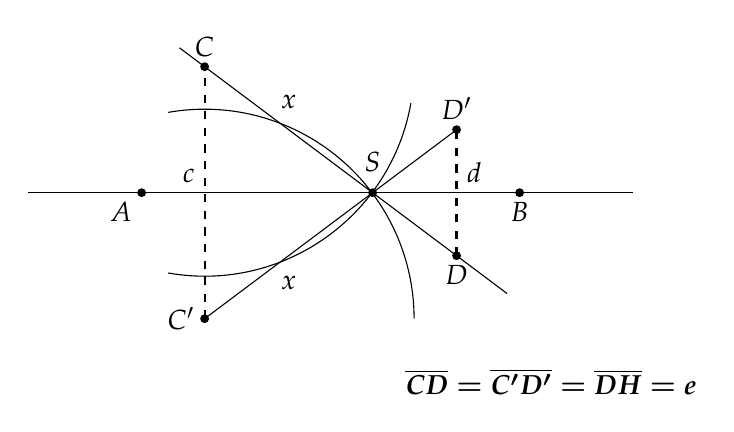
\begin{tikzpicture}[scale=.8]
\coordinate (A) at (-4,0);
\coordinate (B) at (2,0);
\coordinate (C) at (-3,2);
\coordinate (D) at (1,-1);
\coordinate (Cp) at (-3,-2);
\coordinate (Dp) at (1,1);
\fill (A) node[below left] {$A$} circle[radius=2pt];
\fill (B) node[below] {$B$} circle[radius=2pt];
\fill (C) node[above] {$C$} circle[radius=2pt];
\fill (D) node[below] {$D$} circle[radius=2pt];
\fill (Cp) node[left] {$C'$} circle[radius=2pt];
\fill (Dp) node[above] {$D'$} circle[radius=2pt];
\draw[name path=ab] ($(A)!1.3!(B)$) -- ($(B)!1.3!(A)$);
\draw[name path=cd] ($(C)!1.2!(D)$) -- ($(D)!1.1!(C)$);
\path [name intersections={of=ab and cd,by={S}}];
\fill (S) node[above,yshift=4pt] {$S$} circle[radius=2pt];
\draw (Cp) -- (Dp);
\path (C) -- node[above,yshift=4pt] {$x$} (S);
\path (Cp) -- node[below,yshift=-4pt] {$x$} (S);
\path (C) -- node[above left] {$c$} (Cp);
\draw[thick,dashed] (D) -- node[above right] {$d$} (Dp);
\node at (2.5,-3) {\mbox{\boldmath $\overline{CD}=\overline{C'D'}=\overline{DH}=e$}};
\draw[name path=circled] (C) let
  \p1 = ($ (S) - (C) $),
  \n2 = {veclen(\x1,\y1)}
in
  ++(-10:\n2) arc (-10:-100:\n2);

\draw[name path=circlecp] (Cp) let
  \p1 = ($ (S) - (C) $),
  \n2 = {veclen(\x1,\y1)}
in
  ++(100:\n2) arc (100:0:\n2);
\draw[thick,dashed] (Cp) -- (C);
\end{tikzpicture}
\end{center}

%%%%%%%%%%%%%%%%%%%%%%%%%%%%%%%%%%%%%%%%%%%%%%%%%%%%%%%%%%%%%%%

\section{Finding the intersection of a line and a circle}\label{s.line-circle}

\textbf{Given a circle $k=C(M,r)$ and a line $\overline{AB}$, construct their intersections using only a compass.}

Construct $M'$, be the reflection of $M$ about $\overline{AB}$ and the circle $k'=c(M',r)$. The points of intersection of $k,k'$ are the points of intersection of the line $\overline{AB}$ and the circle $k$.  This can be shown by congruent triangles, as indicated by the dotted lines in the diagram.

\begin{center}
\begin{tikzpicture}[scale=.5]
\coordinate (A) at (-7,0);
\coordinate (B) at (8,0);
\coordinate (M) at (0,-2);
\coordinate (Mp) at (0,2);
\fill (A) node[below] {$A$} circle[radius=3pt];
\fill (B) node[below] {$B$} circle[radius=3pt];
\fill (M) node[below left] {$M$} circle[radius=3pt];
\fill (Mp) node[above left] {$M'$} circle[radius=2pt];
\draw[name path=c1] (M) circle[radius=3cm];
\draw[name path=c2] (Mp) circle[radius=3cm];
\draw[name path=ab] ($(A)!1.2!(B)$) -- ($(B)!1.2!(A)$);
\path [name intersections={of=c1 and c2,by={S1,S2}}];
\fill (S1) circle[radius=3pt];
\fill (S2) circle[radius=3pt];
\path[name path=radius1] (M) -- ++(15:4cm);
\path [name intersections={of=c1 and radius1,by={R1}}];
\draw[thick,dashed] (M) -- node[below] {$r$} (R1);
\path[name path=radius2] (Mp) -- ++(40:4cm);
\path [name intersections={of=c2 and radius2,by={R2}}];
\draw[thick,dashed] (Mp) -- node[above] {$r$} (R2);
\fill (R1) circle[radius=3pt];
\fill (R2) circle[radius=3pt];
\draw[thick, dotted] (Mp) -- (M) -- (S1) -- (Mp) -- (S2) -- (M);
\draw (0,0) rectangle +(12pt,12pt);
\end{tikzpicture}
\end{center}

This construction cannot be done if $M$ is on the line $\overline{AB}$. In that case, extend and shorten $\overline{AM}$ by length $r$ as described in Section~\ref{s.add-subtract}. The end points of the extended and shortened segments are the intersections of $k$ with $\overline{AB}$.


\begin{center}
\begin{tikzpicture}[scale=.5]
\coordinate (A) at (-7,0);
\coordinate (B) at (8,0);
\coordinate (M) at (0,0);
\fill (A) node[below] {$A$} circle[radius=3pt];
\fill (B) node[below] {$B$} circle[radius=3pt];
\fill (M) node[below left] {$M$} circle[radius=3pt];
\draw[name path=c1] (M) circle[radius=3cm];
\draw[name path=ab] ($(A)!1.2!(B)$) -- ($(B)!1.2!(A)$);
\path[name path=radius1] (M) -- ++(-30:4cm);
\path [name intersections={of=c1 and radius1,by={R1}}];
\draw[thick,dashed] (M) -- node[below] {$r$} (R1);
\path [name intersections={of=c1 and ab,by={S1,S2}}];
\fill (S1) node[above right] {$\overline{AM}+r$} circle[radius=3pt];
\fill (S2) node[above left] {$\overline{AM}-r$} circle[radius=3pt];
\fill (R1) circle[radius=3pt];
\end{tikzpicture}
\end{center}



\tikzsetfigurename{straightedge-only}
% !TeX root = constructions.tex

\chapter{A Straightedge (with Something Extra) is Sufficient}\label{c.straightedge}

Can every construction with straightedge and compass be done with only a straightedge? The answer is no because lines represent linear equations and cannot represent quadratic equations like circles. In 1822 the French mathematician Jean-Victor Poncelet conjectured that a straightedge only is sufficient, provided that one circle exists in the plane. This was proved in 1833 by the Swiss mathematician Jakob Steiner. In this chapter I present a proof of the theorem based on the proof in problem 34 in \cite{dorrie1} as reworked by Michael Woltermann \cite{dorrie2}.\footnote{I would like to thank Woltermann for permission to use his work.}

Every step of a construction with straightedge and compass is one of these three operations:
\begin{itemize}
\setlength{\itemsep}{0pt}
\item Find the point of intersection of two straight lines.
\item Find the point(s) of intersection of a straight line and a circle.
\item Find the point(s) of intersection of two circles.
\end{itemize}
It is clear that the first operation can be performed with a straightedge only.

What does it mean to perform a construction with straight-edge alone? A circle is defined by a point $O$, its center, and a line segment whose length is the radius $r$, one of whose endpoints is the center. If we can construct the points labeled $X$ and $Y$ in the diagram below, we can claim to have successfully constructed the intersection of a given circle with a given line and of two given circles. The circles drawn with dashed lines in the diagram do not actually appear in the construction. In this chapter, the single existing circle is drawn with a regular line, and the dashed circles are only used to help understand a construction and its proof.
\begin{center}
\begin{tikzpicture}[scale=.9]
\fill (0,0) node[above right] {$O$} circle[radius=1.5pt];
\draw[thick,dashed,name path=circle] (0,0) circle[radius=2cm];
\draw (0,0) -- node[left] {$r$} ++(-60:2cm);
\fill (0,0) ++(-60:2cm) circle[radius=1.5pt];
\draw[name path=line] (-3,-.5) -- ++(20:6cm);
\path [name intersections={of=circle and line,by={X,Y}}];
\fill (X) node[above right,xshift=-2pt,yshift=4pt] {$X$} circle[radius=1.5pt];
\fill (Y) node[above left] {$Y$} circle[radius=1.5pt];
\begin{scope}[xshift=6cm]
\fill (0,0) node[above right] {$O_1$} circle[radius=1.5pt];
\fill (3,0) node[above right] {$O_2$} circle[radius=1.5pt];
\draw[thick,dashed,name path=circle1] (0,0) circle[radius=2cm];
\draw[thick,dashed,name path=circle2] (3,0) circle[radius=2cm];
\draw (0,0) -- node[left] {$r_1$} ++(-60:2cm);
\draw (3,0) -- node[left,below] {$r_2$} ++(-20:2cm);
\fill (3,0) ++(-20:2cm) circle[radius=1.5pt];
\path [name intersections={of=circle1 and circle2,by={X,Y}}];
\fill (X) node[above,yshift=4pt] {$X$} circle[radius=1.5pt];
\fill (Y) node[below,yshift=-4pt] {$Y$} circle[radius=1.5pt];
\end{scope}
\end{tikzpicture}
\end{center}

First we present five auxiliary constructions (Sections~\ref{s.parallel}--\ref{s.root}), and then show how to find the intersection of a line with a circle (Section~\ref{s.line-circle-straight}) and the intersection of two circles (Section~\ref{s.two-circles}).

\newpage

\section{Construct a line parallel to a given line}\label{s.parallel}

\textbf{Given a line $l$ defined by two points $A,B$ and a point $P$ not on the line, construct a line through $P$ that is parallel to $\overline{AB}$.}

There are two cases:
\begin{itemize}
\setlength{\itemsep}{0pt}
\item A ``directed line'': the midpoint $M$ of $\overline{AB}$ is given.
\item Any other line.
\end{itemize}

\textbf{Case 1, directed line}: Construct a ray that extends $AP$ and choose any point $S$ on the ray beyond $P$. Construct the lines $\overline{BP}, \overline{SM}, \overline{SB}$. Label by $O$ the intersection of $\overline{BP}$ with $\overline{SM}$. Construct a ray that extends $\overline{AO}$ and label by $Q$ the intersection of the ray $\overline{AO}$ with $\overline{SB}$.

\begin{center}
\vspace*{-8pt}
\begin{tikzpicture}
\draw[name path=pq] (-4,0) -- (4,0);
\draw (-2,-2) node[below left] {$A$} coordinate (A) -- (2,-2) node[below right] {$B$} coordinate (B);
\fill (A) circle[radius=1.5pt];
\fill (B) circle[radius=1.5pt];
\draw[name path=as] (A) -- ++(50:4cm) node[above] {$S$} coordinate (S);
\fill (S) circle[radius=1.5pt];
\draw[name path=sb] (S) -- (B);
\path [name intersections={of=pq and as,by={P}}];
\path [name intersections={of=pq and sb,by={Q}}];
\fill (P) node[above left] {$P$} circle[radius=1.5pt];
\fill (Q) node[above right] {$Q$} circle[radius=1.5pt];
\draw[name path=pb] (P) -- (B);
\draw[name path=qa] (Q) -- (A);
\path [name intersections={of=pb and qa,by={O}}];
\fill (O) node[right,xshift=2pt] {$O$} circle[radius=1.5pt];
\fill (0,-2) coordinate (M) node[below right] {$M$} circle[radius=1.5pt];
\draw (S) -- (M);
\end{tikzpicture}
\vspace*{-6pt}
\end{center}

\textbf{Claim: $\overline{PQ}$ is parallel to $\overline{AB}$.}

\textbf{Proof:} We will use Ceva's theorem that we proof later.

\textbf{Theorem (Ceva):} Given three line segments from the vertices of a triangle to the opposite edges that intersect in a point ($O$ in the diagram, but $M$ is not necessarily the midpoint of the side), the lengths of the segments satisfy:
\[
\frac{\overline{AM}}{\overline{MB}}\cdot\frac{\overline{BQ}}{\overline{QS}}\cdot\frac{\overline{SP}}{\overline{PA}} = 1\,.
\]

In the construction above, $M$ is the midpoint of $\overline{AB}$, so $\disfrac{\overline{AM}}{\overline{MB}}=1$, so the equation becomes:
\begin{equation}
\frac{\overline{BQ}}{\overline{QS}}=\frac{\overline{PA}}{\overline{SP}}=\frac{\overline{AP}}{\overline{PS}}\,.\label{eq.ceva}
\end{equation}
We will prove that $\triangle ABS \sim \triangle PQS$, so that $\overline{PQ}$ is parallel to $\overline{AB}$ because $\angle ABS = \angle PQS$.
\erh{12pt}
\begin{equationarray*}{rcl}
\overline{BS}&=&\overline{BQ}+\overline{QS}\\
\disfrac{\overline{BS}}{\overline{QS}}&=&\disfrac{\overline{BQ}}{\overline{QS}}+\disfrac{\overline{QS}}{\overline{QS}} = \disfrac{\overline{BQ}}{\overline{QS}}+1\\
\overline{AS}&=&\overline{AP}+\overline{PS}\\
\disfrac{\overline{AS}}{\overline{PS}} &=& \disfrac{\overline{AP}}{\overline{PS}} + \disfrac{\overline{PS}}{\overline{PS}} = \disfrac{\overline{AP}}{\overline{PS}} + 1\,.
\end{equationarray*}
Using Equation~\ref{eq.ceva}:
\[
\disfrac{\overline{BS}}{\overline{QS}}=\disfrac{\overline{BQ}}{\overline{QS}}+1=\disfrac{\overline{AP}}{\overline{PS}}+1=\disfrac{\overline{AS}}{\overline{PS}}\,,
\]
so that $\triangle ABS \sim \triangle PQS$.

\textbf{Proof of Ceva's theorem:} Examine the following diagrams:

\vspace{-4ex}

\begin{center}
\begin{tikzpicture}
\path[name path=pq] (-4,0) -- (4,0);
\draw (-2,-2) node[below left] {$A$} coordinate (A) -- (2,-2) node[below right] {$B$} coordinate (B);
\coordinate (M) at (0,-2);
\draw[name path=as] (A) -- ++(50:4cm) node[above] {$S$} coordinate (S);
\draw[name path=sb] (S) -- (B);
\path [name intersections={of=pq and as,by={P}}];
\path [name intersections={of=pq and sb,by={Q}}];
\path[name path=pb] (P) -- (B);
\path[name path=qa] (Q) -- (A);
\path [name intersections={of=pb and qa,by={O}}];
\draw[fill=gray!40] (B) -- (O) -- (Q);
\draw[fill=gray!70] (S) -- (O) -- (Q);
\draw (B) -- (O) -- (A);
\draw (S) -- (O) -- (A);
\draw (A) -- (B) -- (S) -- cycle;
\draw (S) -- (O);
\draw (B) -- (O);
\fill (A) circle[radius=1.5pt];
\fill (B) circle[radius=1.5pt];
\fill (S) circle[radius=1.5pt];
\fill (Q) node[above right] {$Q$} circle[radius=1.5pt];
\fill (O) node[above left] {$O$} circle[radius=1.5pt];
\path[name path=al1] (O) -- ($(Q)!(O)!(B)$);
\path [name intersections={of=al1 and sb,by={A1}}];
\draw[thick,dashed] (O) -- (A1);
\begin{scope}[xshift=6cm]
\path[name path=pq] (-4,0) -- (4,0);
\draw (-2,-2) node[below left] {$A$} coordinate (A) -- (2,-2) node[below right] {$B$} coordinate (B);
\coordinate (M) at (0,-2);
\draw[name path=as] (A) -- ++(50:4cm) node[above] {$S$} coordinate (S);
\draw[name path=sb] (S) -- (B);
\path [name intersections={of=pq and as,by={P}}];
\path [name intersections={of=pq and sb,by={Q}}];
\draw[name path=pb] (P) -- (B);
\draw[name path=qa] (Q) -- (A);
\path [name intersections={of=pb and qa,by={O}}];
\draw (B) -- (O) -- (Q);
\draw (A) -- (Q) -- (B);
\draw[fill=gray!40] (B) -- (Q) -- (A);
\draw[fill=gray!70] (S) -- (Q) -- (A);
\draw (A) -- (B) -- (S) -- cycle;
\draw (S) -- (O);
\draw (B) -- (O);
\fill (A) circle[radius=1.5pt];
\fill (B) circle[radius=1.5pt];
\fill (S) circle[radius=1.5pt];
\fill (Q) node[above right] {$Q$} circle[radius=1.5pt];
\fill (O) node[above left] {$O$} circle[radius=1.5pt];
\path[name path=al2] (A) -- ($(Q)!(A)!(B)$);
\path [name intersections={of=al2 and sb,by={A2}}];
\draw[thick,dashed] (A) -- (A2);
\end{scope}
\end{tikzpicture}
\end{center}

\vspace{-3ex}

If the altitudes of two triangles are equal, their areas are proportional to the bases. In both diagrams, the altitudes of the gray triangles are equal, so:\footnote{We use the name of a triangle as a shortcut for its area}
\[
\frac{\triangle BQO}{\triangle SQO} = \frac{\overline{BQ}}{\overline{QS}}\;,\quad\quad \frac{\triangle BQA}{\triangle SQA} = \frac{\overline{BQ}}{\overline{QS}}\;.
\]
By subtracting the areas of the indicated triangles, we get the proportion between the gray triangles:

\vspace{-3ex}

\begin{center}
\begin{tikzpicture}
\path[name path=pq] (-4,0) -- (4,0);
\draw (-2,-2) node[below left] {$A$} coordinate (A) -- (2,-2) node[below right] {$B$} coordinate (B);
\coordinate (M) at (0,-2);
\draw[name path=as] (A) -- ++(50:4cm) node[above] {$S$} coordinate (S);
\draw[name path=sb] (S) -- (B);
\path [name intersections={of=pq and as,by={P}}];
\path [name intersections={of=pq and sb,by={Q}}];
\path[name path=pb] (P) -- (B);
\draw[thick,name path=qa] (Q) -- (A);
\path [name intersections={of=pb and qa,by={O}}];
\draw[fill=gray!50] (B) -- (O) -- (A);
\draw[fill=gray!70] (S) -- (O) -- (A);
\draw (B) -- (O) -- (A);
\draw (S) -- (O) -- (A);
\draw (A) -- (B) -- (S) -- cycle;
\draw (S) -- (O);
\draw (B) -- (O);
\fill (A) circle[radius=1.5pt];
\fill (B) circle[radius=1.5pt];
\fill (S) circle[radius=1.5pt];
\fill (Q) node[above right] {$Q$} circle[radius=1.5pt];
\fill (O) node[right,xshift=2pt] {$O$} circle[radius=1.5pt];
\end{tikzpicture}
\end{center}

\[
\frac{\triangle BOA}{\triangle SOA}=\frac{\triangle BQA - \triangle BQO}{\triangle SQA-\triangle SQO} = \frac{\overline{BQ}}{\overline{QS}}\,.
\]
This might look strange at first. We explain it using a simpler notation:
\erh{12pt}
\begin{equationarray*}{rcl}
 \disfrac{c}{d} &=&\disfrac{a}{b}\\
 \disfrac{e}{f} &=&\disfrac{a}{b}\\
c-e &=& \disfrac{ad}{b} - \disfrac{af}{b}=\disfrac{a}{b}(d-f)\\
\disfrac{c-e}{d-f} &=& \disfrac{a}{b}\,.
\end{equationarray*}
Similarly, we can prove:
\[
\frac{\overline{AM}}{\overline{MB}} = \frac{\triangle AOS}{\triangle BOS}\;,\quad\quad \frac{\overline{SP}}{\overline{PA}} =\frac{\triangle SOB}{\triangle AOB}\;,
\]
so:
\[
\frac{\overline{AM}}{\overline{MB}}\frac{\overline{BQ}}{\overline{QS}}\frac{\overline{SP}}{\overline{PA}} = \frac{\triangle AOS}{\triangle BOS}\frac{\triangle BOA}{\triangle SOA}\frac{\triangle SOB}{\triangle AOB}=1\,,
\]
because the order of the vertices in a triangle makes no difference:
\[
\triangle AOS=\triangle SOA,\, \triangle BOA=\triangle AOB,\, \triangle SOB=\triangle BOS\,.
\]
\textbf{End of the proof of Ceva's theorem}

\textbf{Case 2, any other line:} Label the line by $l$ and the existing circle, which we will call the \textbf{fixed circle}, by $c$, where the center of $c$ is $O$ and its radius is $r$. $P$ is the point not on the line through which it is required to construct a line parallel to $l$. Convince yourself that the construction does not depend on the location of the center of the circle or its radius.

Choose $M$, any point on $l$, and construct a ray extending $\overline{MO}$ that intersects the circle at $U,V$.
\begin{center}
\begin{tikzpicture}[scale=.8]
\coordinate (O) at (0,0);
\fill (O) node[below right] {$O$} circle[radius=1.5pt];
\draw[name path=circle] (O) circle[radius=2cm];
\draw[name path=l] (-4,-3) -- node[above, near end] {$l$} +(9,0);
\path[name path=mo] (-2,-3) coordinate (M) -- ($(-2,-3)!1.65!(O)$);
\fill (M) node[below] {$M$} circle[radius=1.5pt];
\path [name intersections={of=circle and mo,by={V,U}}];
\fill (U) node[below,xshift=2pt,yshift=-4pt] {$U$} circle[radius=1.5pt];
\fill (V) node[right,xshift=4pt] {$V$} circle[radius=1.5pt];
\draw (M) -- (U) -- node[left] {$r$} (O) -- node[left] {$r$} (V);
\node at (-1.6,1.6) {$c$};
\fill (-4,1) node[above left] {$P$} circle[radius=1.5pt];
\end{tikzpicture}
\vspace*{-16pt}
\end{center}
This line is a \textbf{directed line} because $O$, the center of the circle, bisects the diameter $\overline{UV}$. Choose a point $A$ on $l$ and use the construction for a directed line to construct a line parallel to $\overline{UV}$, which intersects the circle at $X,Y$.


\begin{center}
\begin{tikzpicture}[scale=.8]
\coordinate (O) at (0,0);
\fill (O) node[below right] {$O$} circle[radius=1.5pt];
\draw[name path=circle] (O) circle[radius=2cm];
\draw[name path=l] (-4,-3) -- node[above,near end,xshift=24pt] {$l$} +(9,0);
\path[name path=mo] (-2,-3) coordinate (M) -- ($(-2,-3)!1.65!(O)$);
\fill (M) node[below] {$M$} circle[radius=1.5pt];
\path [name intersections={of=circle and mo,by={V,U}}];
\fill (U) node[below,xshift=2pt,yshift=-4pt] {$U$} circle[radius=1.5pt];
\fill (V) node[right,xshift=4pt] {$V$} circle[radius=1.5pt];
\draw (M) -- (V);
\path[name path=ax] (-3,-3) coordinate (A) -- ($(-3,-3)!1.8!(-1,0)$);
\fill (A) node[below] {$A$} circle[radius=1.5pt];
\path [name intersections={of=circle and ax,by={Y,X}}];
\fill (X) node[left] {$X$} circle[radius=1.5pt];
\fill (Y) node[above] {$Y$} circle[radius=1.5pt];
\node at (-1.6,1.6) {$c$};
\draw (A) -- (Y);
\fill (-4,1) node[above left] {$P$} circle[radius=1.5pt];
\end{tikzpicture}
\end{center}
Construct the diameters $\overline{XX'}$ and $\overline{YY'}$. Construct the ray from $\overline{X'Y'}$ and label by $B$ its intersection with $l$.
\begin{center}
\begin{tikzpicture}[scale=.8]
\coordinate (O) at (0,0);
\fill (O) node[below right] {$O$} circle[radius=1.5pt];
\draw[name path=circle] (O) circle[radius=2cm];
\draw[name path=l] (-4,-3) -- node[above,near end,xshift=24pt] {$l$} +(9,0);
\path[name path=mo] (-2,-3) coordinate (M) -- ($(-2,-3)!1.65!(O)$);
\fill (M) node[below] {$M$} circle[radius=1.5pt];
\path [name intersections={of=circle and mo,by={V,U}}];
\fill (U) node[below,xshift=2pt,yshift=-4pt] {$U$} circle[radius=1.5pt];
\fill (V) node[right,xshift=4pt] {$V$} circle[radius=1.5pt];
\draw (M) -- (V);
\path[name path=ax] (-3,-3) coordinate (A) -- ($(-3,-3)!1.8!(-1,0)$);
\fill (A) node[below] {$A$} circle[radius=1.5pt];
\path [name intersections={of=circle and ax,by={Y,X}}];
\fill (X) node[left] {$X$} circle[radius=1.5pt];
\fill (Y) node[above] {$Y$} circle[radius=1.5pt];
\node at (-1.6,1.6) {$c$};
\draw (A) -- (Y);
\fill (-4,1) node[above left] {$P$} circle[radius=1.5pt];
\path[name path=xo] (X) -- ($(X)!2.2!(O)$);
\path[name intersections={of=circle and xo,by={Xp}}];
\fill (Xp) node[right,xshift=2pt,yshift=-2pt] {$X'$} circle[radius=1.5pt];
\draw (X) -- (Xp);
\path[name path=yo] (Y) -- ($(Y)!2.2!(O)$);
\path[name intersections={of=circle and yo,by={y,Yp}}];
\fill (Yp) node[below right] {$Y'$} circle[radius=1.5pt];
\draw (Y) -- (Yp);
\path[name path=xy] (Xp) -- ($(Xp)!1.6!(Yp)$);
\path[name intersections={of=l and xy,by={B}}];
\fill (B) node[below] {$B$} circle[radius=1.5pt];
\draw (Xp) -- (B);
\draw[thick,dashed,name path=z] (-4,0) -- (4,0) node[above,near end,xshift=40pt] {$l'$};
\path[name intersections={of=ax and z,by={Z}}];
\path[name intersections={of=xy and z,by={Zp}}];
\fill (Z) node[above left] {$Z$} circle[radius=1.5pt];
\fill (Zp) node[below right] {$Z'$} circle[radius=1.5pt];
\end{tikzpicture}
\end{center}
\textbf{$l$ is a directed line because $M$ is the bisector of $\overline{AB}$, so a line can be constructed through $P$ parallel to $l$.}

\textbf{Proof:} $\overline{OX}, \overline{OX'}, \overline{OY}, \overline{OY'}$ are all radii of the circle and $\angle XOY = \angle X'OY'$ since they are vertical angles. $\triangle XOY\cong\triangle X'OY'$ by side-angle-side. Define (not construct!) $l'$ to be a line through $O$ parallel to $l$ that intersects $\overline{XY}$ at $Z$ and $\overline{X'Y'}$ at $Z'$. $\angle XOZ=\angle X'OZ'$ because they are vertical angles, so $\triangle XOZ\cong\triangle X'OZ'$ by angle-side-angle and $\overline{ZO}=\overline{OZ'}$. $\overline{AMOZ}$ and $\overline{BMOZ'}$ are parallelograms (quadrilaterals with opposite sides parallel), so $\overline{AM}=\overline{ZO}=\overline{OZ'}=\overline{MB}$.

\textbf{Corollary:} Given a line segment $\overline{AB}$ and a point $P$ not on the line. It is possible to construct a line through $P$ that is parallel to $\overline{AB}$ and whose length is equal to the length of $\overline{AB}$. In other words, it is possible to copy $\overline{AB}$ parallel to itself with $P$ as one of its endpoints.

\textbf{Proof:} We have proved that it is possible to construct a line $m$ through $P$ parallel to $\overline{AB}$ and a line $n$ through $B$ to parallel to $\overline{AP}$. The quadrilateral $\overline{ABQP}$ is a parallelogram so opposite sides are equal $\overline{AB}=\overline{PQ}$.
\begin{center}
\begin{tikzpicture}[scale=.8]
\coordinate (P) at (0,0);
\coordinate (Q) at (3,0);
\coordinate (A) at (-2,2.5);
\coordinate (B) at (1,2.5);
\draw ($(P)!-.6!(Q)$) -- node[above,near end,xshift=36pt] {$m$} ($(P)!1.8!(Q)$);
\fill (P) node[below] {$P$} circle[radius=1.5pt];
\fill (Q) node[below left] {$Q$} circle[radius=1.5pt];
\draw ($(A)!-.6!(B)$) -- node[above,near end,xshift=40pt] {$l$} ($(A)!2.5!(B)$);
\fill (A) node[above left] {$A$} circle[radius=1.5pt];
\fill (B) node[above right] {$B$} circle[radius=1.5pt];
\draw (A) -- (P);
\draw ($(B)!-.3!(Q)$) -- node[above,near end,xshift=24pt,yshift=-24pt] {$n$} ($(B)!1.4!(Q)$);
\end{tikzpicture}
\end{center}

\newpage

\section{Construct a perpendicular to a given line}\label{s.perp}

\textbf{Construct a perpendicular line segment through a point $P$ to a given line $l$ ($P$ is not on $l$).}

Construct (Section~\ref{s.parallel}) a line $l'$ parallel to $l$ that intersects the \textbf{fixed circle} at $U,V$. Construct the diameter $\overline{UOU'}$ and chord $\overline{VU'}$.
\begin{center}
\begin{tikzpicture}[scale=.8]
\coordinate (O) at (0,0);
\coordinate (P) at (3.5,.6);
\node at (-1.6,1.6) {$c$};
\draw[name path=circle] (O) circle[radius=2cm];
\draw[name path=l] (-4,-3) -- node[above,near end,xshift=45pt] {$l$} ++(9,0);
\draw[name path=lp] (-3,-1) -- node[above,near end,xshift=45pt] {$l'$} ++(7,0);
\fill (O) node[above left] {$O$} circle[radius=1.5pt];
\fill (P) node[right] {$P$} circle[radius=1.5pt];
\path[name intersections={of=circle and lp,by={U,V}}];
\fill (U) node[below left] {$U$} circle[radius=1.5pt];
\fill (V) node[below right] {$V$} circle[radius=1.5pt];
\path[name path=d] (U) -- ($(U)!2.3!(O)$);
\path[name intersections={of=circle and d,by={Up}}];
\draw (U) -- (Up);
\fill (Up) node[above right] {$U'$} circle[radius=1.5pt];
\draw (Up) -- (V);
\path[name path=p] (P) -- ++(0,-4);
\draw[name intersections={of=p and l,by={X}}];
\fill (X) circle[radius=1.5pt];
\draw[thick,dashed] (P) -- (X);
\draw ($(U)!.9!(V)$) -- ++(0,.3) -| (V);
\end{tikzpicture}
\end{center}

$\angle UVU'$ is an angle that subtends a semicircle so it is a right angle. Therefore, $\overline{VU'}$ is perpendicular to $\overline{UV}$ and $l$. Construct (Section~\ref{s.parallel}) the parallel to $\overline{VU'}$ through $P$.

\section{Copy a line segment in a given direction}\label{s.copy}

The corollary at the end of Section~\ref{s.parallel} shows that it is possible to copy a line segment parallel to itself. Here we show that it is possible to copy a line segment in the direction of another line. The meaning of  ``direction'' is that the line defined by two points $A',H'$ defines an angle $\theta$ relative to some axis. The task is to copy $\overline{PQ}$ to $\overline{AS}$ so that $\overline{AS}$ will have the same angle $\theta$ relative to the same axis. In the diagram $\overline{PQ}$ is on the $x$-axis but that is of no importance.
\begin{center}
\begin{tikzpicture}[scale=.7]
\coordinate (A) at (0,0);
\coordinate (P) at (1cm,-1.5);
\coordinate (Q) at (2.5cm,-1.5);
\draw (P) -- (Q);
\fill (P) node[left] {$P$} circle[radius=1.5pt];
\fill (Q) node[right] {$Q$} circle[radius=1.5pt];
\coordinate (A1) at (-3,1);
\draw (A1) -- ++(60:3cm) coordinate (H1);
\draw[thick,dashed] (A1) -- ++(0:1.5cm);
\fill (A1) node[left] {$A'$} circle[radius=1.5pt];
\fill (H1) node[left] {$H'$} circle[radius=1.5pt];
\draw[thick,dashed] (A) -- ++(60:1.5cm) coordinate (S);
\fill (S) node[left] {$S$} circle[radius=1.5pt];
\draw[thick,dashed] (A) -- ++(1.5,0);
\fill (A) node[left] {$A$} circle[radius=1.5pt];
\node[above right,xshift=4pt] at (A1) {$\theta$};
\node[above right,xshift=4pt] at (A) {$\theta$};
\end{tikzpicture}
\end{center}
By Section~\ref{s.parallel} it is possible to construct a line segment $\overline{AH}$ so that $\overline{AH}\|\overline{A'H'}$ and to construct a line segment $\overline{AK}$ so that $\overline{AK}\|\overline{PQ}$.

\vspace{-1ex}

\begin{center}
\begin{tikzpicture}[scale=.7]
\coordinate (A) at (0,0);
\coordinate (P) at (1,-1.5);
\coordinate (Q) at (2.5,-1.5);
\draw (P) -- (Q);
\fill (P) node[left] {$P$} circle[radius=1.5pt];
\fill (Q) node[right] {$Q$} circle[radius=1.5pt];
\coordinate (A1) at (-3,1);
\draw (A1) -- ++(60:3cm) coordinate (H1);
\draw[thick,dashed] (A1) -- ++(0:1.5cm);
\fill (A1) node[left] {$A'$} circle[radius=1.5pt];
\fill (H1) node[left] {$H'$} circle[radius=1.5pt];
\draw (A) -- ++(60:3cm) coordinate (H);
\fill (H) node[left] {$H$} circle[radius=1.5pt];
\draw (A) -- ++(1.5,0) coordinate (K);
\fill (K) node[below right] {$K$} circle[radius=1.5pt];
\draw (A) -- (K);
\fill (A) node[left] {$A$} circle[radius=1.5pt];
\node[above right,xshift=4pt] at (A1) {$\theta$};
\node[above right,xshift=4pt] at (A) {$\theta$};
\end{tikzpicture}
\end{center}
$\angle HAK=\theta$ so it remains to find a point $S$ on $\overline{AH}$ so that $\overline{AS}=\overline{PQ}$.

\vspace{-1ex}

\begin{center}
\begin{tikzpicture}[scale=.7]
\coordinate (A) at (0,0);
\coordinate (P) at (1,-1.5);
\coordinate (Q) at (2.5,-1.5);
\draw (P) -- (Q);
\fill (P) node[left] {$P$} circle[radius=1.5pt];
\fill (Q) node[right] {$Q$} circle[radius=1.5pt];
\coordinate (A1) at (-3,1);
\draw (A1) -- ++(60:3cm) coordinate (H1);
\fill (A1) node[left] {$A'$} circle[radius=1.5pt];
\fill (H1) node[left] {$H'$} circle[radius=1.5pt];
\draw (A) -- ++(60:3cm) coordinate (H);
\fill (A) node[left] {$A$} circle[radius=1.5pt];
\fill (H) node[left] {$H$} circle[radius=1.5pt];
\coordinate (O) at (6,1);
\node at (4.8,3.4) {$c$};
\draw[name path=circle] (O) circle[radius=2.5cm];
\fill (O) node[above left] {$O$} circle[radius=1.5pt];
\draw (A) -- ++(1.5,0) coordinate (K);
\fill (K) node[below right] {$K$} circle[radius=1.5pt];
\draw (A) -- (K);
\path[name path=u] (O) -- ++(60:2.5cm);
\path[name path=v] (O) -- ++(2.5,0);
\path[name intersections={of=circle and u,by={U}}];
\path[name intersections={of=circle and v,by={V}}];
\fill (U) node[above right] {$U$} circle[radius=1.5pt];
\fill (V) node[right] {$V$} circle[radius=1.5pt];
\draw (O) -- (U) -- (V) -- cycle;
\path (A) -- ++(60:1.5cm) coordinate (S);
\fill (S) node[right] {$S$} circle[radius=1.5pt];
\draw (K) -- ($(K)!1.8!(S)$);
\draw (A) -- (S);
\node[above right,xshift=4pt] at (A) {$\theta$};
\node[above right,xshift=4pt] at (O) {$\theta$};
\node[above right,xshift=4pt] at (A1) {$\theta$};
\draw[thick,dashed] (A1) -- ++(1.5,0);
\end{tikzpicture}
\end{center}
\vspace{-1ex}

Construct two radii $\overline{OU}, \overline{OV}$ of the fixed circle which are parallel to $\overline{AH}, \overline{AK}$, respectively, and construct a ray through $K$ parallel to $\overline{UV}$. Label its intersection with $\overline{AH}$ by $S$. 

\textbf{Claim: $\overline{AS}=\overline{PQ}$}

\textbf{Proof:} By construction, $\overline{AH}\|\overline{OU}$ and $\overline{AK}\|\overline{OV}$, so $\angle SAK=\theta=\angle UOV$. $\overline{SK}\|\overline{UV}$ and $\triangle SAK\sim\triangle UOV$ by angle-angle-angle, $\triangle UOV$ is isosceles, because $\overline{OU}, \overline{OV}$ are radii of the same circle. Therefore, $\triangle SAK$ is isosceles and $\overline{AS}=\overline{AK}=\overline{PQ}$.

\section{Construct a line segment relative to three other line segments}\label{s.relative}

\textbf{Given line segments of lengths $n, m, s$, construct a segment of length $x=\disfrac{n}{m}s$.}

The three line segments are located at arbitrary positions and directions in the plane.

\begin{center}
\begin{tikzpicture}[scale=.9]
\draw (0,0) -- node[above] {$s$} ++(30:1.5cm);
\draw (2,1.2) -- node[above] {$m$} ++(-10:2.5cm);
\draw (-2,1.5) -- node[above] {$n$} ++(5:2cm);
\fill (0,0) circle[radius=1.5pt];
\fill (2,1.2) circle[radius=1.5pt];
\fill (-2,1.5) circle[radius=1.5pt];
\fill (0,0) ++(30:1.5cm) circle[radius=1.5pt];
\fill (2,1.2) ++(-10:2.5cm) circle[radius=1.5pt];
\fill (-2,1.5) ++(5:2cm) circle[radius=1.5pt];
\end{tikzpicture}
\end{center}

Choose a point $A$ and construct two rays $\overline{AB}, \overline{AC}$. By the construction in Section~\ref{s.copy} it is possible to construct points $M,N,S$ such that $\overline{AM}= m$, $\overline{AN} =n$, $\overline{AS}=s$. Construct a line through $N$ parallel to $\overline{MS}$ which intersects $\overline{AC}$ at $X$ and label its length by $x$. $\triangle MAS\sim\triangle NAX$ by angle-angle-angle so:
\[
\frac{m}{n}=\frac{s}{x}\,\quad\quad x=\frac{n}{m}s\,.
\]
\begin{center}
\begin{tikzpicture}
\coordinate (A) at (0,0);
\draw[name path=ac] (A) node[left] {$A$} -- ++(7,0) node[right] {$C$};
\draw (A) -- ++(40:5cm) node[right] {$B$};
\fill (A) circle[radius=1.5pt];
\fill (A) ++(40:5cm) circle[radius=1.5pt];
\fill (A) ++(7,0) circle[radius=1.5pt];
\path (A) -- node[above,xshift=-2pt] {$m$} ++(40:3cm) coordinate (M) node[above left] {$M$};
\path (A) -- ++(40:4cm) coordinate (N) node[above left] {$N$};
\fill (M) circle[radius=1.5pt];
\fill (N) circle[radius=1.5pt];
\path[name path=ms] (M) -- ++(-50:3.5cm);
\path[name path=nx] (N) -- ++(-50:4cm);
\path[name intersections={of=ac and ms,by={S}}];
\path[name intersections={of=ac and nx,by={X}}];
\fill (S) circle[radius=1.5pt] node[below] {$S$};
\fill (X) circle[radius=1.5pt] node[below] {$X$};
\path (A) -- node[below] {$s$} (S);
\draw (S) -- (M);
\draw (X) -- (N);
\node at (7,2.5) {$\overline{AN}=n$};
\node at (7,2) {$\overline{AX}=x$};

\draw[<->] ($(A)+(0,-.8)$) -- node[fill=white] {$x$} ($(X)+(0,-.8)$);
\draw[<->] ($(A)+(-.6,.8)$) -- node[fill=white] {$n$} ++(40:3.9cm);
\end{tikzpicture}
\end{center}

\section{Construct a square root}\label{s.root}

\textbf{Given line segments of lengths $a,b$, construct a segment of length $\sqrt{ab}$.}

We want to express $x=\sqrt{ab}$ in the form $\disfrac{n}{m}s$ in order to use the result of Section~\ref{s.relative}.
\begin{itemize}
\setlength{\itemsep}{0pt}
\item For $n$ we use $d$, the diameter of the fixed circle.
\item For $m$ we use $t=a+b$ which can be constructed from $a,b$ as shown in Section~\ref{s.copy}.
\item We define $s=\sqrt{hk}$ where $h,k$ are defined as expressions on the lengths $a,b,t,d$, and we will show how it is possible to construct a line segment of length $\sqrt{ab}$.
\end{itemize}
Define $h=\disfrac{d}{t}a$, $k=\disfrac{d}{t}b$ and and compute:
\[
x=\sqrt{ab}=\sqrt{\frac{th}{d}\frac{tk}{d}}=\sqrt{\left(\frac{t}{d}\right)^2hk}=\frac{t}{d}hk=\frac{t}{d}s\,.
\]
We also compute:
\[
h+k = \frac{d}{t}a + \frac{d}{t}b = \frac{d(a+b)}{t} = \frac{dt}{t} = d\,.
\]

By Section~\ref{s.copy} construct $\overline{HA}= h$ on a diameter $\overline{HK}$ of the fixed circle. From $h+k=d$ we have $\overline{AK}=k$:
\begin{center}
\begin{tikzpicture}[scale=.8]
\coordinate (O) at (0,0);
\coordinate (H) at (-3,0);
\coordinate (K) at (3,0);
\node at (-2.4,2.4) {$c$};
\draw (H) -- (K);
\draw[name path=circle] (O) circle[radius=3cm];
\fill (O) node[below] {$O$} circle[radius=1.5pt];
\fill (H) node[left] {$H$} circle[radius=1.5pt];
\fill (K) node[right] {$K$} circle[radius=1.5pt];
\path[name path=as] (1,0) coordinate (A) -- ++(0,3.2);
\fill (A) node[below] {$A$} circle[radius=1.5pt];
\path[name intersections={of=circle and as,by={S}}];
\fill (S) node[above] {$S$} circle[radius=1.5pt];
\draw (A) -- node[right] {$s$} (S);
\path (H) -- node[above] {$h$} (A);
\path (A) -- node[above] {$k$} (K);
\draw[thick,dashed] (O) -- node[left,xshift=-2pt] {$\disfrac{d}{2}$} (S);
\node at (.5,-1.5) {$\disfrac{d}{2}-k$};
\draw[->] (.5, -1.2) -- ++(0,1);
\draw (.8,0) -- ++(0,.2) -- ++(.2,0);
\end{tikzpicture}
\end{center}
By Section~\ref{s.perp} construct a perpendicular to $\overline{HK}$ at $A$ and label the intersection of this line with the circle by $S$. $\overline{OS}=\overline{OK}=\disfrac{d}{2}$ because they are radii of the circle and $\overline{OA}=\disfrac{d}{2}-k$. By Pythagoras's theorem:
\erh{12pt}
\begin{equationarray*}{rcl}
s^2=\overline{SA}^2 &=& \left(\disfrac{d}{2}\right)^2 - \left(\disfrac{d}{2}-k\right)^2\\
&=& \left(\disfrac{d}{2}\right)^2 - \left(\disfrac{d}{2}\right)^2 + 2\disfrac{dk}{2} - k^2\\
&=& k(d-k) = kh\\
s&=&\sqrt{hk}\,.
\end{equationarray*}
Now $x=\disfrac{t}{d}s$ can be constructed by Section~\ref{s.relative}.

\section{Construct the points of intersection of a line and a circle}\label{s.line-circle-straight}

\textbf{Given a line $l$ and a circle $c(O,r)$, construct their points of intersection.}

\begin{center}
\begin{tikzpicture}[scale=.7]
\coordinate (O) at (0,0);
\node at (2.6,-2) {$c$};
\draw[thick,dashed,name path=circle] (O) circle[radius=3cm];
\fill (O) node[below right] {$O$} circle[radius=2pt];
\draw (O) -- node[above] {$r$} ++(-130:3cm) coordinate (R);
\fill (R) circle[radius=2pt];
\draw[name path=l] (O) ++(170:4cm) -- node[below, near end,xshift=40pt,yshift=12pt] {$l$} ++(20:8cm);
\path[name intersections={of=circle and l,by={Y,X}}];
\fill (X) circle[radius=2pt];
\fill (Y) circle[radius=2pt];
\end{tikzpicture}
\end{center}

By Section~\ref{s.perp} it is possible to construct a perpendicular from the center of the circle $O$ to the line $l$. Label the intersection of $l$ with the perpendicular by $M$. $M$ bisects the chord $\overline{XY}$, where $X, Y$ are the intersections of the line with the circle. $2s$ is the length of the chord $\overline{XY}$. Note that $s,X,Y$ in the diagram are just definitions: we haven't constructed them yet.

\begin{center}
\begin{tikzpicture}[scale=.7]
\coordinate (O) at (0,0);
\node at (2.6,-2) {$c$};
\draw[thick,dashed,name path=circle] (O) circle[radius=3cm];
\fill (O) node[below right] {$O$} circle[radius=2pt];
\path (O) -- node[above] {$r$} ++(-130:3cm) coordinate (R);
\fill (R) node[right,yshift=2pt,xshift=2pt] {$R$} circle[radius=2pt];
\draw[name path=l] (O) ++(170:4cm) --
  node[below, near end,xshift=40pt,yshift=12pt] {$l$} ++(20:8cm);
\path[name intersections={of=circle and l,by={Y,X}}];
\fill (X) node[above left] {$X$} circle[radius=2pt];
\fill (Y) node[above right] {$Y$} circle[radius=2pt];
\draw[thick,dashed] (O) -- node[below] {$r$} (X);
\path (X) -- ($(X)!.5!(Y)$) coordinate (M);
\fill (M) node[above] {$M$} circle[radius=2pt];
\draw[thick,dashed] (O) -- node[right] {$t$} (M);
\path (X) -- node[above] {$s$} (M);
\path (M) -- node[above] {$s$} (Y);
\draw (O) ++(170:4cm) -- ++(20:3.1cm) -- ++(-70:10pt) -- ++(20:10pt);

\draw[thick,dotted] (O) -- node[below] {$t$} +(50:2);
\draw[thick,dotted] (O) -- node[below] {$t$} +(-130:2) coordinate (RT);
\fill (RT) circle(2pt);
\draw (RT) -- ($(RT)+(-130:1cm)$);
\end{tikzpicture}
\end{center}
$\triangle OMX$ is a right triangle, so $s^2=r^2-t^2=(r+t)(r-t)$. $r$ is the given radius of the circle and $t$ is defined s the length of $\overline{OM}$, the line segment between $O$ and $M$. By Section~\ref{s.copy} it is possible to construct a line segment of length $t$ from $O$ in the two directions $\overline{OR}$ and $\overline{RO}$. The result is two line segments of length $r+t,r-t$.

Section~\ref{s.root} shows how to construct a line segment of length $s=\sqrt{(r+t)(r-t)}$. By Section~\ref{s.copy} it is possible to construct line segments of length $s$ from $M$ along the given line $l$ in both directions. Their other endpoints are the points of intersection of $l$ and $c$.


\section{Construct the points of intersection of two circles}\label{s.two-circles}

\textbf{Given two circles $c(O_1,r_1), c(O_2,r_2)$, construct their points of intersection.}

With a straightedge it is possible to construct a line segment $\overline{O_1O_2}$ that connects the two centers. Label its length $t$.

\begin{center}
\begin{tikzpicture}[scale=1.1]
\coordinate (O1) at (0,0);
\coordinate (O2) at (2.5,0);
\fill (O1) node[below left] {$O_1$} circle[radius=1pt];
\fill (O2) node[below right] {$O_2$} circle[radius=1pt];
\draw[thick,dashed,name path=circle1] (O1) circle[radius=2cm];
\draw[thick,dashed,name path=circle2] (O2) circle[radius=1.6cm];
\path [name intersections={of=circle1 and circle2,by={X,Y}}];
\draw (O1) -- node[above] {$r_1$} ++(160:2cm);
\draw (O2) -- node[above] {$r_2$} ++(30:1.6cm);
\fill (O1) ++(160:2cm) circle[radius=1pt];
\fill (O2) ++(30:1.6cm) circle[radius=1pt];
\draw (O1) -- (O2);
\node at (-1.7,1.6) {$c_1$};
\node at (3.8,1.4) {$c_2$};
\draw[<->] (0,-1) -- node[fill=white] {$t$} (2.5,-1);
\node at (6,0) {$t=\overline{O_1O_2}$};
\end{tikzpicture}
\end{center}

Label by $A$ be the point of intersection of $\overline{O_1O_2}$ and $\overline{XY}$, and label the lengths $q=\overline{O_1A}$, $x=\overline{XA}$. Note that we have not constructed $A$, but if we succeed in constructing the lengths $q,x$, by Section~\ref{s.copy} we can construct $A$ at length $q$ from $O_1$ in the direction $\overline{O_1O_2}$. 
\begin{center}
\begin{tikzpicture}[scale=1.1]
\coordinate (O1) at (0,0);
\coordinate (O2) at (2.5,0);
\fill (O1) node[below left] {$O_1$} circle[radius=1pt];
\fill (O2) node[below right] {$O_2$} circle[radius=1pt];
\draw[thick,dashed,name path=circle1] (O1) circle[radius=2cm];
\draw[thick,dashed,name path=circle2] (O2) circle[radius=1.6cm];
\path [name intersections={of=circle1 and circle2,by={X,Y}}];
\fill (X) node[above,yshift=4pt] {$X$} circle[radius=1pt];
\fill (Y) node[below,yshift=-4pt] {$Y$} circle[radius=1pt];
\draw[thick,dashed] (O1) -- node[above,xshift=-4pt] {$r_1$} (X);
\draw[thick,dashed] (O2) -- node[above,xshift=4pt] {$r_2$} (X);
\draw[name path=oo] (O1) -- (O2);
\node at (-1.7,1.6) {$c_1$};
\node at (3.8,1.4) {$c_2$};
\draw[name path=xy] (X) -- (Y);
\path[name intersections={of=xy and oo,by={A}}];
\fill (A) node[below left] {$A$} circle[radius=1pt];
\draw (A) rectangle +(7pt,7pt);
\path (O1) -- node[below,xshift=-2pt] {$q$} (A);
\path (X) -- node[left,yshift=-2pt] {$x$} (A);
\draw[<->] (0,-1) -- node[fill=white] {$t$} (2.5,-1);
\node at (6,.5) {$t=\overline{O_1O_2}$};
\node at (6,0) {$q=\overline{O_1A}$};
\node at (6,-.5) {$x=\overline{XA}$};
\end{tikzpicture}
\end{center}
By Section~\ref{s.perp} a perpendicular to $\overline{O_1O_2}$ at $A$ can be constructed and again by Section~\ref{s.copy} it is possible to construct line segments of length $x$ from $A$ is both directions along the perpendicular. Their other endpoints are  the points of intersection of the circles.

\textbf{Constructing the length $q$:} Define $d=\sqrt{r_1^2+t^2}$, the hypotenuse of a right triangle. It can be constructed from $r_1,t$, the known lengths of the other two sides. On any line construct a line segment $\overline{RS}$ of length $r_1$, then a perpendicular to $\overline{RS}$ through $R$, and finally, a line segment $\overline{RT}$ of length $t$ through $R$ on the perpendicular. The length of the hypotenuse $\overline{ST}$ is $d$. This right triangle can be constructed anywhere in the plane, not necessarily near the circles.

By the law of cosines for $\triangle O_1O_2X$:
\erh{12pt}
\begin{equationarray*}{rcl}
r_2^2 &=& r_1^2 + t^2 - 2r_1t\cos\angle XO_1O_2\\
&=& r_1^2 + t^2 - 2tq\\
q&=&\disfrac{(d+r_2)(d-r_2)}{2t}\,.
\end{equationarray*}
By Section~\ref{s.copy} these lengths can be constructed and by Section~\ref{s.relative} $q$ can be constructed from $d+r_2,d-r_2,2t$.

\textbf{Constructing the length x:} $\triangle AO_1X$ is a right triangle, so $x=\sqrt{r_1^2-q^2}=\sqrt{(r_1+q)(r_1-q)}$. By Section~\ref{s.copy} $h =r_1+ q,k= r_1 - q$ can be constructed, as can $x=\sqrt{hk}$ by Section~\ref{s.root}.



\tikzsetfigurename{axioms}
% !TeX root = constructions.tex

\part{Origami}\label{p.origami}

\chapter{Axioms}\label{c.axioms}

Each axiom states that a \emph{fold} exists that will place given points and lines onto points and lines, such that certain properties hold. The term fold comes from the origami operation of folding a piece of paper, but here it is used to refer the geometric line that would be created by folding the paper.

The axioms are called the \emph{Huzita-Hatori axioms} \cite{wiki:hh}, although their final form resulted from the work of several other mathematicians. Lee \cite[Chapter~4]{hwa} is a good overview of the mathematics of origami, while Martin \cite[Chapter~10]{martin} is a formal development. Formal definitions are given in \cite[Chapter~10]{martin}. The reader should be aware that, \emph{by definition}, folds result in \emph{reflections}. Given a point $p$, its reflection around a fold $l$ results in a point $p'$, such that $l$ is the perpendicular bisector of the line segment $\overline{pp'}$:

%\begin{figure}[H]
\begin{center}
\begin{tikzpicture}
\coordinate (P1) at (2,2);
\coordinate (P1P) at (6,4);
\coordinate (mid) at (4,3);
\draw[rotate=30] (mid) rectangle +(8pt,8pt);
\coordinate (m1) at ($(P1)!.5!(mid)$);
\coordinate (m2) at ($(mid)!.5!(P1P)$);
\draw[thick] (m1) -- +(120:4pt);
\draw[thick] (m1) -- +(-60:4pt);
\draw[thick] (m2) -- +(120:4pt);
\draw[thick] (m2) -- +(-60:4pt);
\draw[thick] (P1) -- (P1P);
\draw[very thick,dashed] (4.7,1.6) -- node[very near end,right,yshift=4pt] {$l$} (3.5,4);
\fill (P1) circle(2pt) node[above left] {$p$};
\fill (P1P) circle(2pt) node[above left] {$p'$};
\fill (mid) circle(2pt);% node[below,xshift=-2pt,yshift=-8pt] {$p_i$};
\draw[very thick,dotted,->,bend right=50] (2,1.8) to (6,3.8);
\end{tikzpicture}
\end{center}
%\end{figure}

In the diagrams, given lines are solid, folds are dashed, auxiliary lines are dotted, and dotted arrows indicate the direction of folding the paper.

\newpage

\section{Axiom 1}\label{s.ax1}


\textbf{Axiom} 
Given two distinct points $p_1=(x_1,y_1)$, $p_2=(x_2,y_2)$, there is a unique fold $l$ that passes through both of them.

%\begin{figure}[H]
\begin{center}
\begin{tikzpicture}[scale=1.2]
\draw[step=10mm,white!50!black,thin] (-1,-1) grid (8,6);
\draw[thick] (-1,0) -- (8,0);
\draw[thick] (0,-1) -- (0,6);
\foreach \x in {0,...,8}
  \node at (\x-.2,-.2) {\sm{\x}};
\foreach \y in {1,...,6}
  \node at (-.2,\y-.3) {\sm{\y}};
\coordinate (P1) at (2,2);
\coordinate (P2) at (6,4);
\draw[very thick,dashed] ($(P1)!-.75!(P2)$) -- node[very near end,below] {$l$} ($(P1)!1.5!(P2)$);
\fill (P1) circle(2pt) node[above left] {$p_1$};
\fill (P2) circle(2pt) node[above left] {$p_2$};

\draw[very thick,dotted,->,bend left=30] (2,5) to (4,1);
\end{tikzpicture}
\end{center}
%\end{figure}

\textbf{Derivation of the equation of the fold}

The equation of fold $l$ is derived from the coordinates of $p_1$ and $p_2$: the slope is the quotient of the differences of the coordinates and the intercept is derived from $p_1$:
\begin{equation}
y - y_1 = \disfrac{y_2-y_1}{x_2-x_1}(x-x_1)\,.
\end{equation}

\vspace*{-3ex}
%\newpage

\textbf{Example}

Let  $p_1=(2,2), p_2=(6,4)$. The equation of $l$ is:
\begin{form}{2}
y-2&=&\disfrac{4-2}{6-2}(x-2)\\
y&=&\disfrac{1}{2}x+1\,.
\end{form}

%%%%%%%%%%%%%%%%%%%%%%%%%%%%%%%%%%%%%%%%%%%%%%%%%%%%%%%%%%%%%%%%
\newpage

\section{Axiom 2}\label{s.ax2}


\textbf{Axiom} 
Given two distinct points $p_1=(x_1,y_1)$, $p_2=(x_2,y_2)$, there is a unique fold $l$ that places $p_1$ onto $p_2$.

%\begin{figure}[H]
\begin{center}
\begin{tikzpicture}[scale=1.2]
\draw[step=10mm,white!50!black,thin] (-1,-1) grid (8,6);
\draw[thick] (-1,0) -- (8,0);
\draw[thick] (0,-1) -- (0,6);
\foreach \x in {0,...,8}
  \node at (\x-.2,-.2) {\sm{\x}};
\foreach \y in {1,...,6}
  \node at (-.2,\y-.3) {\sm{\y}};
\coordinate (P1) at (2,2);
\coordinate (P2) at (6,4);
\coordinate (mid1) at ($(P1)!.5!(P2)$);
\coordinate (mid2) at ($(P1)!.5!(P2)+(-1,2)$);

\draw[rotate=30] (mid1) rectangle +(8pt,8pt);

\draw[very thick,dotted] (P1) -- (P2);
\draw[very thick,dashed] ($(mid1)!-1.4!(mid2)$) -- node[very near end,left,yshift=-12pt] {$l$} ($(mid1)!1.4!(mid2)$);
\fill (P1) circle(2pt) node[above left] {$p_1$};
\fill (P2) circle(2pt) node[above left] {$p_2$};

\draw[very thick,dotted,->,bend right=50] (2,1.8) to (6,3.8);
\end{tikzpicture}
\end{center}
%\end{figure}

\textbf{Derivation of the equation of the fold}

The fold $l$ is the perpendicular bisector of $\overline{p_1p_2}$. Its slope is the negative reciprocal of the slope of the line connecting $p_1$ and $p_2$. $l$ passes through the midpoint between the points:
\begin{equation}
y - \disfrac{y_1+y_2}{2} = -\disfrac{x_2-x_1}{y_2-y_1}\left(x-\disfrac{x_1+x_2}{2}\right)\,.\label{eq.midpoint1}
\end{equation}

\textbf{Example}

Let $p_1=(2,2), p_2=(6,4)$. The equation of $l$ is:
\begin{form}{2}
y-\left(\disfrac{2+4}{2}\right)&=&-\disfrac{6-2}{4-2}\left(x-\left(\disfrac{2+6}{2}\right)\right)\\
y&=&-2x+11\,.
\end{form}

%%%%%%%%%%%%%%%%%%%%%%%%%%%%%%%%%%%%%%%%%%%%%%%%%%%%%%%%%%%%%%%%
\newpage

\section{Axiom 3}\label{s.ax3}


\textbf{Axiom} 
Given two lines $l_1$ and $l_2$, there is a fold $l$ that places $l_1$ onto $l_2$.

%\begin{figure}[H]
\begin{center}
\begin{tikzpicture}[scale=1.2]
\draw[step=10mm,white!50!black,thin] (-1,-1) grid (8,7);
\draw[thick] (-1,0) -- (8,0);
\draw[thick] (0,-1) -- (0,7);
\foreach \x in {0,...,8}
  \node at (\x-.2,-.2) {\sm{\x}};
\foreach \y in {1,...,7}
  \node at (-.2,\y-.3) {\sm{\y}};
\coordinate (L1a) at (2,2);
\coordinate (L1b) at (4,6);
\draw[thick] (L1a) -- node[very near start,right,yshift=-4pt] {$l_1$} (L1b);
\draw[thick,dotted,name path=l1] ($(L1a)!-.75!(L1b)$) -- ($(L1a)!1.25!(L1b)$);
\coordinate (L2a) at (7,1);
\coordinate (L2b) at (4,4);
\draw[thick] (L2a) -- (L2b);
\draw[thick,dotted,name path=l2] ($(L2a)!-.3!(L2b)$) -- node[very near start,above,xshift=4pt,yshift=2pt] {$l_2$} ($(L2a)!2!(L2b)$);
\path [name intersections = {of = l1 and l2, by = {PM}}];
\fill (PM) circle(2pt) node[below left,xshift=-9pt,yshift=-7pt] {$p_i$};

\node[above right,xshift=10pt,yshift=4pt] at (PM) {$\alpha$};
\node[below right,xshift=10pt] at (PM) {$\alpha$};
\node[above left,xshift=-3pt,yshift=12pt] at (PM) {$\beta$};
\node[above right,xshift=-3pt,yshift=12pt] at (PM) {$\beta$};

\coordinate (B1a) at (0,4.13);
\coordinate (B1b) at (6,5.1);
\draw[very thick,dashed] ($(B1a)!-.15!(B1b)$) -- node[very near start,above] {$l_{f_1}$}  ($(B1a)!1.35!(B1b)$);

\coordinate (B2a) at (3,6.73);
\coordinate (B2b) at (4,.57);
\draw[very thick,dashed] ($(B2a)!-.05!(B2b)$) -- node[very near end,right,xshift=4pt,yshift=6pt] {$l_{f_2}$} ($(B2a)!1.25!(B2b)$);

\draw[very thick,dotted,->,bend right=50] (6,2.2) to (4.5,6.7);
\draw[very thick,dotted,->,bend left=50] (6.2,1.6) to (1.8,1.3);
\end{tikzpicture}
\end{center}
%\end{figure}

\textbf{Derivation of the equation of the fold}

If the lines are parallel, let $l_1$ be $y=mx+b_1$ and let $l_2$ be $y=mx+b_2$. The fold is the line parallel to $l_1,l_2$ and halfway between them $y=mx+\disfrac{b_1+b_2}{2}$.

If the lines intersect, let $l_1$ be $y=m_1x+b_1$ and let $l_2$ be $y=m_2x+b_2$.

\textbf{Derivation of the point of intersection}

$p_i=(x_i,y_i)$, the point of intersection of the two lines, is:
\vspace{-2ex}
\begin{form}{1.8}
m_1x_i+b_2&=&m_2x_i+b_2\\
x_i &=& \disfrac{b_2-b_1}{m_1-m_2}\\
y_i &=&m_1x_i+b_1\,.
\end{form}
\vspace{-2ex}

\textbf{Example}
 
Let $l_1$ be $y=2x-2$ and let $l_2$ be $y=-x+8$. The point of intersection is:
\begin{form}{2}
x_i&=&\disfrac{8-(-2)}{2-(-1)}=\disfrac{10}{3}\approx 3.33\\
y_i &=& 2\cdot\disfrac{10}{3}-2=\disfrac{14}{3}\approx 4.67\,.
\end{form}
\textbf{Derivation of the equation of the slope of the angle bisector}

The two lines form an angle at their point of intersection, actually, two pairs of vertical angles. The folds are the bisectors of these angles.

If the angle of line $l_1$ relative to the $x$-axis is $\theta_1$ and the angle of line $l_2$ relative to the $x$-axis is $\theta_2$, then the fold is the line which makes an angle of $\theta_b=\disfrac{\theta_1+\theta_2}{2}$ with the $x$-axis.

$\tan\theta_1=m_1$ and $\tan\theta_2=m_2$ are given and $m_b$, the slope of the angle bisector, is:
\[
m_b=\tan\theta_b=\tan\disfrac{\theta_1+\theta_2}{2}\,.
\]
The derivation requires the use of two trigonometric identities that we derive here:
\begin{form}{1.3}
\tan (\theta_1+\theta_2) &=& \disfrac{\sin(\theta_1+\theta_2)}{\cos(\theta_1+\theta_2)}\\
&=&\disfrac{\sin\theta_1\cos\theta_2+\cos\theta_1\sin\theta_2}{\cos\theta_1\cos\theta_2-\sin\theta_1\sin\theta_2}\\
&=&\disfrac{\sin\theta_1+\cos\theta_1\tan\theta_2}{\cos\theta_1-\sin\theta_1\tan\theta_2}\\
&=&\disfrac{\tan\theta_1+\tan\theta_2}{1-\tan\theta_1\tan\theta_2}\,.
\end{form}

We use this formula to obtain a quadratic equation in $\tan(\theta/2)$:
\begin{form}{1.3}
\tan \theta=\disfrac{\tan(\theta/2)+\tan(\theta/2)}{1-\tan^2(\theta/2)}\\
\tan\theta \,(\tan(\theta/2))^2 \;+\; 2\,(\tan (\theta/2)) \;-\;\tan \theta = 0\,.
\end{form}
Its solutions are:
\[
\tan(\theta/2) = \disfrac{-1\pm\sqrt{1+\tan^2\theta}}{\tan\theta}\,.
\]
First derive $m_s$, the slope of $\theta_1+\theta_2$:
\[
m_s=\tan(\theta_1+\theta_2)= \disfrac{m_1+m_2}{1-m_1m_2}\,.
\]
Then derive $m_b$, the slope of the angle bisector:
\begin{form}{1.3}
m_b&=& \tan\disfrac{\theta_1+\theta_2}{2}\\
&=&\disfrac{-1\pm\sqrt{1+\tan^2(\theta_1+\theta_2)}}{\tan (\theta_1+\theta_2)}\\
&=&\disfrac{-1\pm\sqrt{1+m_s^2}}{m_s}\,.
\end{form}
\textbf{Example}
For the lines $y=2x-2$ and $y=-x+8$, the slope of the angle bisector is:
\begin{form}{1.3}
m_s=\disfrac{2+(-1)}{1-(2 \cdot -1)}=\disfrac{1}{3}\\
m_b=\disfrac{-1\pm\sqrt{1+(1/3)^2}}{1/3}=-3\pm \sqrt{10}\approx -6.16,\; 0.162\,.
\end{form}

\textbf{Derivation of the equation of the fold}

Let us derive equation of the fold $l_{f_1}$ with the positive slope; we know the coordinates of the intersection of the two lines $m_i=\left(\disfrac{10}{3},\disfrac{14}{3}\right)$:
\begin{form}{2}
\disfrac{14}{3} &=& (-3+\sqrt{10}) \cdot \disfrac{10}{3} + b\\ b&=&\disfrac{44-10\sqrt{10}}{3}\\
y&=& (-3+\sqrt{10})x + \disfrac{44-10\sqrt{10}}{3}\approx 0.162x+4.13\,.
\end{form}


%%%%%%%%%%%%%%%%%%%%%%%%%%%%%%%%%%%%%%%%%%%%%%%%%%%%%%%%%%%%%%%%
\newpage

\section{Axiom 4}\label{s.ax4}


\textbf{Axiom} 
Given a point $p_1$ and a line $l_1$, there is a unique fold $l$ perpendicular to $l_1$ that passes through point $p_1$.
%\begin{figure}[H]
\begin{center}
\begin{tikzpicture}[scale=1.2]
\draw[step=10mm,white!50!black,thin] (-1,-1) grid (8,7);
\draw[thick] (-1,0) -- (8,0);
\draw[thick] (0,-1) -- (0,7);
\foreach \x in {0,...,8}
  \node at (\x-.2,-.2) {\sm{\x}};
\foreach \y in {1,...,7}
  \node at (-.2,\y-.3) {\sm{\y}};
\coordinate (L1a) at (2,0);
\coordinate (L1b) at (5,6);
\draw[thick] (L1a) -- node[very near start,right,yshift=-4pt] {$l_1$} ($(L1a)!1.15!(L1b)$);
\fill (2,6) circle (2pt) node[above right] {$p_1$};
\draw[thick,dashed] (0,7) -- node[very near end,above right] {$l$} (8,3);
\coordinate (intersection) at (4.4,4.8);
\draw[rotate=-30] (intersection) rectangle +(8pt,8pt);

\draw[very thick,dotted,->,bend left=50] (5.4,6.3) to (3.7,3);
\end{tikzpicture}
\end{center}
%\end{figure}

\textbf{Derivation of the equation of the fold}

Let $l_1$ be $y = m_1x + b_1$ and let $p_1=(x_1,y_1)$.  $l$ is perpendicular to $l_1$ so its slope is $-\disfrac{1}{m_1}$. Since it passes through $p_1$, we can compute the intercept $b$ and write down its equation:
\begin{form}{2}
y_1=-\disfrac{1}{m} x_1 + b\\
b= \disfrac{(my_1+x_1)}{m}\\
y=-\disfrac{1}{m} x +\disfrac{(my_1+x_1)}{m}\,.
\end{form}
\textbf{Example}

Let $p_1=(2,6)$ and let $l_1$ be $y=2x-4$. The equation of the fold $l$ is:
\[
y=-\disfrac{1}{2}x + \disfrac{2\cdot 6 + 2}{2}=-\disfrac{1}{2}x + 7\,.
\]


%%%%%%%%%%%%%%%%%%%%%%%%%%%%%%%%%%%%%%%%%%%%%%%%%%%%%%%%%%%%%%%%
\newpage

\section{Axiom 5}\label{s.ax5}


\textbf{Axiom} 
Given two points $p_1,p_2$ and a line $l_1$, there is a fold $l$ that places $p_1$ onto $l_1$ and passes through $p_2$.

%\begin{figure}[H]
\begin{center}
\begin{tikzpicture}[scale=1.1]
\draw[step=10mm,white!50!black,thin] (-1,-1) grid (9,9);
\draw[thick] (-1,0) -- (9,0);
\draw[thick] (0,-1) -- (0,9);
\foreach \x in {0,...,9}
  \node at (\x-.2,-.2) {\sm{\x}};
\foreach \y in {1,...,9}
  \node at (-.2,\y-.3) {\sm{\y}};
\coordinate (L1a) at (0,3);
\coordinate (L1b) at (8,-1);
\draw[thick] (L1a) -- node[near end,below right,xshift=8pt,yshift=-8pt] {$l_1$} (L1b);
\coordinate (P1) at (2,8);
\fill (P1) circle (2pt) node[above left] {$p_1$};
\coordinate (P2) at (4,4);
\fill (P2) circle (2pt) node[above left,yshift=4pt] {$p_2$};
\draw[thick,dotted,name path=L1] (8,-1) -- (-1,3.5);
\node[very thick,dotted,draw, name path = circle] at (P2)
    [circle through = (P1)] {};

\path [name intersections = {of = circle and L1, by = {P1P,P1PP}}];
\fill (P1P) circle (2pt) node[above left,xshift=-2pt,yshift=4pt] {$p_1'$};
\fill (P1PP) circle (2pt) node[above left,yshift=6pt] {$p_1''$};

\coordinate (f1) at (0,6);
\draw[thick,dashed] ($(f1)!-.25!(P2)$) -- node[very near end,above] {$l_{f_2}$} ($(f1)!2.25!(P2)$);
\coordinate (f2) at (0,2);
\draw[thick,dashed] ($(f2)!-.25!(P2)$) -- node[very near end,below,yshift=-2pt] {$l_{f_1}$} ($(f2)!2.25!(P2)$);

\draw[very thick,dotted,->,bend left=50] (2.2,7.8) to (-.2,3.2);
\draw[very thick,dotted,->,bend left=50] (2.4,7.85) to (6.1,.2);
\end{tikzpicture}
\end{center}
%\end{figure}


For a given pair of points and a line, there may be zero, one or two folds.

\textbf{Derivation of the equations of the reflections}

Let $l$ be a fold through $p_2$ and $p_1'$ be the reflection of $p_1$ around $l$. The length of $\overline{p_1p_2}$ equals the length of $\overline{p_2p_1}'$. The locus of points at distance $\overline{p_1p_2}$ \emph{from} $p_2$ is the circle centered at $p_2$ whose radius is the length of $\overline{p_1p_2}$. The intersections of this circle with the line $l_1$ give the possible points $p_1'$.

Let $l_1$ be $y=m_1x + b_1$ and let $p_1=(x_1,y_1)$, $p_2=(x_2,y_2)$. The equation of the circle centered at $p_2$ with radius the length of $\overline{p_1p_2}$ is:
\begin{form}{1.5}
(x-x_2)^2 + (y-y_2)^2 = r^2\,,\quad \textrm{where}\\
r^2= (x_2-x_1)^2 + (y_2-y_1)^2\,.
\end{form}
Substituting the equation of the line into the equation for the circle:
\[
(x-x_2)^2+((m_1x+b_1)-y_2)^2=(x-x_2)^2+(m_1x+(b_1-y_2))^2=r^2\,,
\]
we obtain a quadratic equation for the $x$-coordinates of the possible intersections:
\begin{equation}
x^2(1+m_1^2) \,+\, 2(-x_2+m_1b-m_1y_2)x \,+\, (x_2^2 + (b_1^2 - 2b_1y_2+y_2^2)-r^2)=0\,.\label{eq.intersections}
\end{equation}
The quadratic equation has at most two solutions $x_1',x_1''$ and we can compute $y_1',y_1'')$ from $y=m_1x+b_1$. The reflected points are $p_1'=(x_1',y_1')$, $p_1''=(x_1'',y_1'')$.

\textbf{Example}

Let $p_1=(2,8)$, $p_2=(4,4)$ and let $l_1$ be $y=-\disfrac{1}{2}x +3$. The equation of the circle is:
\[
(x-4)^2 + (y-4)^2 = r^2=(4-2)^2+(4-8)^2=20\,.
\]
Substitute the equation of the line into the equation of the circle and simplify to obtain a quadratic equation for the $x$-coordinates of the intersections (or use Equation~\ref{eq.intersections}):
\begin{form}{1.5}
(x-4)^2 + \left(\left(-\disfrac{1}{2}x+3\right)-4\right)^2&=&20\\
\disfrac{5}{4}x^2-7x-3 &=&0\\
5x^2 -28x -12&=&0\\
(5x+2)(x-6)&=&0\,.
\end{form}
The two points of intersection are:
\[
p_1'=\left(-\disfrac{2}{5},\disfrac{16}{5}\right) = (-0.4,3.2)\,,\quad p_1''=(6,0)\,.
\]

\textbf{Derivation of the equations of the folds}

The folds will be the perpendicular bisectors of $\overline{p_1p_1'}$ and $\overline{p_1p_1''}$. The equation of a perpendicular bisector is given by Equation~\ref{eq.midpoint1}, repeated here with for $p_1'$:
\begin{equation}
y - \disfrac{y_1+y_1'}{2} = -\disfrac{x_1'-x_1}{y_1'-y_1}\left(x-\disfrac{x_1+x_1'}{2}\right)\,.\label{eq.midpoint2}
\end{equation}

\textbf{Example}


For $p_1=(2,8)$ and $p_1'=\left(-\disfrac{2}{5},\disfrac{16}{5}\right)$, the equation of the fold $l_{f_1}$  is:
\begin{form}{2}
y-\disfrac{8+(16/5)}{2}&=&-\disfrac{(-2/5)-2}{(16/5)-8}\left(x-\disfrac{2+\left(-2/5\right)}{2}\right)\\
y&=&-\disfrac{1}{2}x+6\,.
\end{form}

For $p_1=(2,8)$ and $p_1''=(6,0)$, the equation of the fold $l_{f_2}$ is:
\begin{form}{2}
y-\disfrac{8+0}{2}&=&-\disfrac{6-2}{0-8}\left(x-\disfrac{2+6}{2}\right)\\
y&=&\disfrac{1}{2}x+2\,.
\end{form}

%%%%%%%%%%%%%%%%%%%%%%%%%%%%%%%%%%%%%%%%%%%%%%%%%%%%%%%%%%%%%%%%

\newpage

\section{Axiom 6}\label{s.ax6}

\textbf{Axiom}                          
Given two points $p_1$ and $p_2$ and two lines $l_1$ and $l_2$, there is a fold $l$ that places $p_1$ onto $l_1$ and $p_2$ onto $l_2$.

%\begin{figure}[H]
\begin{center}
\begin{tikzpicture}[scale=.9]
\draw[step=10mm,white!50!black,thin] (-7,-7) grid (7,5);
\draw[thick] (-7,0) -- (7,0);
\draw[thick] (0,-7) -- (0,5);
\foreach \x in {-6,...,7}
  \node at (\x-.3,-.2) {\sm{\x}};
\foreach \y in {1,...,5}
  \node at (-.2,\y-.3) {\sm{\y}};
\foreach \y in {-6,...,-1}
  \node at (-.3,\y-.3) {\sm{\y}};
  
\coordinate (P1) at (0,4);
\fill (P1) circle (3pt) node[above left,xshift=-2pt] {$p_1$};
\coordinate (P2) at (0,-6);
\fill (P2) circle (3pt) node[above left,xshift=-2pt,yshift=2pt] {$p_2$};

\coordinate (P1P) at (3.1,2);
\fill (P1P) circle (3pt) node[above right,xshift=-2pt] {$p_1'$};
\coordinate (P2P) at (-6.12,-2);
\fill (P2P) circle (3pt) node[below right,xshift=2pt] {$p_2'$};

\coordinate (P1PP) at (-3.1,2);
\fill (P1PP) circle (3pt) node[above right,xshift=-2pt] {$p_1''$};
\coordinate (P2PP) at (6.12,-2);
\fill (P2PP) circle (3pt) node[below right,xshift=2pt] {$p_2''$};

\draw[very thick] (-7,2) -- node[very near start,above,xshift=-34pt] {$l_1$} (7,2);
\draw[very thick] (-7,-2) -- node[very near start,below,xshift=-34pt] {$l_2$} (7,-2);

\draw[domain=-4.8:4.8,samples=50,very thick,dotted] plot (\x,{-.13*\x*\x-4});
\draw[domain=-2.8:2.8,samples=50,very thick,dotted] plot (\x,{.25*\x*\x+3});

\draw[very thick,dashed] (-5,-7) -- (2.95,5);
\draw[very thick,dashed] (-3,5) -- (4.95,-7);

\draw[very thick,dotted,->,bend left=50] (.2,4.1) to (3,2.2);
\draw[very thick,dotted,->,bend left=50] (-.3,-6.1) to (-6.1,-2.2);

\draw[very thick,dotted,->,bend right=50] (-.2,4.1) to (-3,2.2);
\draw[very thick,dotted,->,bend right=50] (.3,-6.1) to (6.1,-2.2);
\end{tikzpicture}
\end{center}
%\end{figure}

For a given pair of points and pair of lines, there may be zero, one, two or three folds.

A fold that places $p_i$ onto $l_i$ is a line such that the distance from $p_i$ to the line is equal to the distance from $l_i$ to the line. The locus of points that are equidistant from a point $p_i$ and a line $l_i$ is a parabola with focus $p_i$ and directrix $l_i$. A fold is any line tangent to that parabola. A detailed justification of this claim is given below.

For a fold to simultaneously place $p_1$ onto $l_1$ and $p_2$ onto $l_2$, it must be a tangent common to the two parabolas.

The formula for an arbitrary parabola is quite complex, so we limit the presentation to parabolas with the the $y$-axis as the axis of symmetry. This is not a significant limitation because for any parabola there is a rigid motion that moves the parabola so that its axis of symmetry is the $y$-axis.

An example will also be given where one of the parabolas has the $x$-axis as its axis of symmetry.

\newpage

\textbf{Derivation of the equation a fold}

Let $(0,f)$ be the focus of a parabola with directrix $y=d$. Define $p=f-d$, the signed length of the line segment between the focus and the directrix.\footnote{We have been using the notation $p_i$ for points; the use of $p$ here might be confusing but it is the standard notation. The formal name for $p$ is one-half the \emph{latus rectum}.} If the vertex of the parabola is on the $x$-axis, the equation of the parabola is $y=\disfrac{x^2}{2p}$. To move the parabola up or down the $y$-axis so that its vertex is at $(0,h)$, add $h$ to the equation of the parabola: $y=\disfrac{x^2}{2p}+h$.
\begin{center}
\begin{tikzpicture}[scale=1]
\draw (-6,0) -- node[very near start,below,xshift=-32pt] {$x$-\textsf{axis}}(6,0);
\draw (0,-3) -- node[very near start,right,yshift=-20pt] {$y$-\textsf{axis}}(0,4.5);
\draw[very thick] (-6,-2) -- node[near start,below] {\textsf{directrix} $\quad y=-2$} (6,-2);
\draw[domain=-5:5,samples=50,very thick,dotted] plot (\x,{\x*\x/8+1});
\coordinate (F) at (0,4);
\fill (F) circle (2pt) node[left,xshift=-2pt,yshift=0pt] {$(0,f)=(0,4)$} node[above left,xshift=-2pt,yshift=4pt] {\textsf{focus}};
\fill (0,-2) circle (2pt);
\fill (0,1) circle (2pt) node[below left] {\textsf{vertex}} node[below left,yshift=-10pt] {$(0,1)$};
\draw[<->] (2,-1.9) -- node[fill=white] {$p=6$} +(0,5.8);
\draw[<->] (1,.1) -- node[fill=white] {$h=1$} +(0,.8);
\end{tikzpicture}
\end{center}
Define $a=2ph$ so that the equation of the parabola is:
\begin{form}{1.5}
y=\disfrac{x^2}{2p}+\disfrac{a}{2p}\\
x^2-2py+a=0\,.
\end{form}
The equation of the parabola in the diagram above is:
\begin{form}{1}
x^2-2\cdot 6\,y + 2\cdot 6 \cdot 1=0\\
x^2-12y +12=0\,.
\end{form}
Substitute the equation of an \emph{arbitrary} line $y=mx+b$ into the equation for the parabola to obtain an equation for the points of intersection of the line and the parabola:
\begin{form}{1.5}
x^2-2p(mx+b)+a=0\\
x^2+(-2mp)x+(-2pb+a)=0\,.
\end{form}
The line will be tangent to the parabola iff this quadratic equation has \emph{exactly one} solution iff its discriminant is zero:
\[
(-2mp)^2\:-\:4\cdot 1\cdot (-2pb+a)=0\,,
\]
which simplifies to:
\begin{equation}
m^2p^2+2pb-a=0\,.\label{eq.disc}
\end{equation}

This is the equation with variable $m$ for the slopes of tangents to the parabola. There are an infinite number of tangents because for each $m$, there is some $b$ that makes the line a tangent by moving it up or down.\footnote{Except of course for a line parallel to the axis of symmetry.}

To obtain the common tangents to both parabolas, the equations for the two parabolas have two unknowns and can be solved for $m$ and $b$.


\textbf{Example}

Parabola 1: focus $(0,4)$, directrix $y=2$, vertex $(0,3)$, $p=2$, $a=2\cdot 2\cdot 3=12$. The equation of the parabola is:
\[
\begin{array}{l}
x^2-2\cdot 2y +12=0\,.
\end{array}
\]
Substituting into Equation~\ref{eq.disc} and simplifying:
\[
m^2+b-3=0\,.
\]
Parabola 2: focus $(0,-4)$, directrix $y=-2$, vertex $(0,-3)$, $p=-2$, $a=2\cdot -2\cdot -3=12$. The equation of the parabola is:
\[
x^2-2\cdot (-2)y+12=0\,.
\]
Substituting into Equation~\ref{eq.disc} and simplifying:
\[
m^2-b-3=0\,.
\]
The solutions of the two equations:
\begin{form}{1.5}
m^2+b-3=0\\
m^2-b-3=0\,,
\end{form}
are $m=\pm\sqrt{3}\approx \pm 1.73$ and $b=0$. There are two common tangents that are the folds:
\[
y=\sqrt{3}x\,,\quad y=-\sqrt{3}x\,.
\]

\textbf{Example}

Parabola 1 is unchanged.

Parabola 2: focus $(0,-6)$, directrix $y=-2$, vertex $(0,-4)$, $p=-4$, $a=2\cdot -4\cdot -4=32$. The equation of the parabola is:
\[
x^2-2\cdot (-4)y +32=0\,.
\]
Substituting into Equation~\ref{eq.disc} and simplifying:
\[
2m^2-b-4=0\,.
\]
The solutions of the two equations:
\begin{form}{1.5}
m^2+b-3=0\\
2m^2-b-4=0\,,
\end{form}
are $m=\pm\sqrt{\disfrac{7}{3}}\approx \pm 1.53$ and $b=\disfrac{2}{3}$. There are two common tangents that are folds:
\[
y=\sqrt{\disfrac{7}{3}}x+\disfrac{2}{3}\,,\quad y=-\sqrt{\disfrac{7}{3}}x+\disfrac{2}{3}\,.
\]

%%%%%%%%%%%%%%%%%%%%%%%%%%%%%%%%%%%%%%%%%%%%%%%%%%%%%%%%%%%%%%%%

\textbf{Example}

Let us now define a parabola whose axis of symmetry is the $x$-axis.

Parabola 1 is unchanged.

Parabola 2: focus $(4,0)$, directrix $x=2$, vertex $(3,0)$, $p=2$, $a=2\cdot 2\cdot 3=12$. The equation of the parabola is:
\[
y^2-4x+12 = 0\,.
\]
Note that this is an equation with $x$ and $y^2$ instead of $x^2$ and $y$, so we can't use Equation~\ref{eq.disc} and we must perform the derivation again.

Substitute the equation for a line:
\begin{form}{1.5}
(mx+b)^2-4x+12=0\\
m^2x^2+(2mb-4)x+(b^2+12)=0\,,
\end{form}
set the discriminant equal to zero and simplify:
\begin{form}{1.5}
(2mb-4)^2\:-\:4m^2(b^2+12)=0\\
-3m^2-mb+1=0\,.
\end{form}
If we try to solve the two equations:
\begin{form}{1.5}
m^2+b-3=0\\
-3m^2-mb+1=0\,,
\end{form}
we obtain a cubic equation with variable $m$:
\begin{equation}
m^3-3m^2-3m+1=0\,.\label{eq.cubic}
\end{equation}
Since a cubic equation has at least one and at most three (real) solutions, there can be one, two or three common tangents. There can also be no common tangents if the two equations have no solution, for example, if one parabola is ``contained'' with another: $y=x^2$, $y=x^2+1$.

The formula for solving cubic equations is quite complicated, so I used a calculator on the internet and obtained three solutions:
\[
m=3.73\,, \;m=-1\,, \; m=0.27\,.
\]
Choosing $m=0.27$, $b=3-m^2=2.93$, and the equation of the fold is:
\[
y=0.27x+2.93\,.
\]

From the form of Equation~\ref{eq.cubic}, we might guess that $1$ or $-1$ is a solution:
\begin{form}{1.4}
1^3-3\cdot 1^2-3\cdot 1+1=-4\\
(-1)^3-3\cdot (-1)^2-3\cdot(-1)+1=0\,.
\end{form}
Divide Equation~\ref{eq.cubic} by $m-(-1)=m+1$ to obtain the quadratic equation $m^2-4m+1$ whose roots are $2\pm\sqrt{3}\approx 3.73, 0.27$.


%%%%%%%%%%%%%%%%%%%%%%%%%%%%%%%%%%%%%%%%%%%%%%%%%%%%%%%%%%%%%%%%

\bigskip

\textbf{Derivation of the equations of the reflections}

We derive the position of the reflection $p_1'=(x_1',y_1')$ of $p_1=(x_1,y_1)$ around some tangent line $l_t$ whose equation is $y=m_tx+b_t$. The derivation is identical for any tangent and for $p_2$.

To reflect $p_1$ around $l_t$, we find the line $l_p$ with equation $y=m_px+b_p$ that is perpendicular to $l_t$ and passes through $p_1$;
\begin{form}{2}
y=-\disfrac{1}{m_t}x+b_p\\
y_1=-\disfrac{1}{m_t}x_1+b_p\\
y=\disfrac{-x}{m_t}+\left(y_1+\disfrac{x_1}{m_t}\right)\,.
\end{form}
Next we find the intersection $p_t=(x_t,y_t)$ of $l_t$ and $l_p$:
\begin{form}{3}
m_tx_t+b_t=\disfrac{-x_t}{m_t}+\left(y_1+\disfrac{x_1}{m_t}\right)\\
x_t=\disfrac{\left(y_1+\disfrac{x_1}{m_t}-b_t\right)}{\left(m_t+\disfrac{1}{m_t}\right)}\\
y_t=m_tx_t+b_t\,.
\end{form}
The reflection $p_1'$ is easy to derive because the intersection $p_t$ is the midpoint between $p_1$ and its reflection $p_1'$:
\begin{form}{2}
x_t=\disfrac{x_1+x_1'}{2}\,,\quad y_t=\disfrac{y_1+y_1'}{2}\\
x_1'=2x_t-x_1\,,\quad y_1'=2y_t-y_1\,.
\end{form}

\newpage

\textbf{Example}

$p_1=(0,4)$, $l_1$ is $y=\sqrt{3}x$:

\begin{form}{2.2}
x_t=\disfrac{\left(4+\disfrac{0}{\sqrt{3}}-0\right)}{\left(\sqrt{3}+\disfrac{1}{\sqrt{3}}\right)}=\sqrt{3}\\
y_t=\sqrt{3}\sqrt{3}+0=3\\
x_1'=2x_t-x_1=2\sqrt{3}-0=2\sqrt{3}\approx 3.46\\
y_1'=2y_t-y_1=2\cdot 3 - 4 = 2\,.
\end{form}


\bigskip

\textbf{A fold is any tangent to a parabola}


Students are usually introduced to parabolas as the graphs of second degree equations:
\[
y=ax^2+bx+c\,.
\]
However, parabolas can be defined geometrically: given a point, the \emph{focus}, and a line, the \emph{directrix}, the locus of points equidistant from the focus and the directrix defines a parabola.


The following diagram shows the focus---the large dot at $p=(0,f)$, and the directrix---the thick line whose equation is $y=-f$. The resulting parabola is shown as a dotted curve. Its vertex $p_2$ is at the origin of the axes.

%\begin{figure}[H]
\begin{center}
\begin{tikzpicture}[scale=1.1]
\draw (-6,0) -- node[very near start,below,xshift=-32pt] {$x$-\textsf{axis}} (6,0);
\draw (0,-3) -- node[very near start,right,yshift=-20pt] {$y$-\textsf{axis}} (0,4.5);
\draw[ultra thick] (-6,-2) -- node[near start,below] {\textsf{directrix} $\quad y=-f$} (6,-2);
\draw[domain=-6:6,samples=50,very thick,dotted] plot (\x,{\x*\x/8});
\coordinate (F) at (0,2);
\fill (F) circle (3pt) node[above left,xshift=-2pt,yshift=15pt] {$(0,f)$} node[above left,xshift=-2pt,yshift=30pt] {\textsf{focus}} node[above right] {$p$};
\fill (0,0) circle (1.5pt) node[below right] {$p_2$};
\fill (0,-2) circle (1.5pt);
\fill (2,-2) circle (1.5pt);
\fill (3,-2) circle (1.5pt);
\fill (5,-2) circle (1.5pt);
\coordinate (FP) at (-5,-2);
\fill (FP) circle (1.5pt) node[below] {$p'$};
\coordinate (F1) at (2,.5);
\fill (F1) circle (1.5pt) node[below right] {$p_3$};
\coordinate (F2) at (3,1.125);
\fill (F2) circle (1.5pt) node[below right] {$p_4$};
\coordinate (F3) at (5,3.125);
\fill (F3) circle (1.5pt) node[below right] {$p_5$};
\coordinate (F4) at (-5,3.125);
\fill (F4) circle (1.5pt) node[above right] {$p_1$};
\draw (F) -- node[left] {$a_2$} (0,0) -- node[left] {$a_2$} (0,-2);
\draw (F) -- node[near end,left] {$a_3$} (F1) -- node[left] {$a_3$} (2,-2);
\draw (F) -- node[near end,above] {$a_4$} (F2) -- node[left] {$a_4$} (3,-2);
\draw (F) -- node[above] {$a_5$} (F3) -- node[left] {$a_5$} (5,-2);
\draw (F) -- node[above] {$a_1$} (F4) -- node[left] {$a_1$} (FP);
\draw[thick,dashed] ($(F4)!-.4!(-2.5,0)$) -- node[very near end,right,xshift=2pt] {$l$} ($(F4)!1.8!(-2.5,0)$);
\draw[very thick,dotted] (F) -- (FP);
\coordinate (H) at (-2.5,0);
\node[above,xshift=1pt] at (H) {$?$};
\draw[rotate=36] (H) rectangle +(10pt,10pt);
\path (FP) -- node[above,yshift=2pt] {$b?$} (H) -- node[above,yshift=2pt] {$b?$} (F);
\draw (0,-2) rectangle +(8pt,8pt);
\draw (2,-2) rectangle +(8pt,8pt);
\draw (3,-2) rectangle +(8pt,8pt);
\draw (5,-2) rectangle +(8pt,8pt);
\draw (-5,-2) rectangle +(8pt,8pt);
\end{tikzpicture}
\end{center}
%\end{figure}

\newpage

We have selected five points $p_i$, $i=1,\ldots,5$ on the parabola. Each point $p_i$ is at a distance of $a_i$ from both the focus and from the directrix. Drop a perpendicular from $p_1$ to the directrix and let $p'$ be the intersection of the perpendicular and the directrix. Since $p_1$ is on the parabola, $\overline{p'p_1}=\overline{p_1p}=a_1$. We claim that the tangent $l$ to the parabola at $p_1$ (dashed line) is a fold that reflects $p$ onto $p'$.

We have to prove the $l$ is the perpendicular bisector of $\overline{pp'}$. Let us extract a simplified diagram:
\begin{center}
\begin{tikzpicture}[scale=1.1]
\draw[thick] (-6.4,0) -- node[very near start,below,xshift=-20pt] {$x$-\textsf{axis}} (1,0);
\draw[thick] (0,-3) -- node[very near start,right,yshift=-20pt] {$y$-\textsf{axis}} (0,3.5);
\draw[thick] (-6.4,-2) -- (1,-2);
\coordinate (F) at (0,2);
\fill (F) circle (1.5pt) node[right] {$p\;\;$ \textsf{focus}};
\fill (0,0) circle (1.5pt) node[below right] {$p_2$};
\coordinate (FP) at (-5,-2);
\fill (FP) circle (1.5pt) node[below] {$p'$};
\path (FP) -- node[below,yshift=-2pt] {\textsf{directrix}} (0,-2);
\fill (0,-2) circle (1.5pt) node[below right] {$s$};
\coordinate (F4) at (-5,3.125);
\fill (F4) circle (1.5pt) node[above right] {$p_1$};
\draw (F) -- node[right] {$a_2$} (0,0) -- node[right] {$a_2$} (0,-2);
\draw (F) -- node[above] {$a_1$} (F4) -- (FP);
\draw[<->] ($(F4)+(-.5,-.1)$) -- node[fill=white] {$a_1$}($(FP)+(-.5,.1)$);
\draw[thick,dashed] ($(F4)!-.15!(-2.5,0)$) -- node[very near end,right,xshift=2pt] {$l$} ($(F4)!1.8!(-2.5,0)$);
\draw[very thick,dotted] (F) -- (FP);
\coordinate (H) at (-2.5,0);
\node[above,xshift=1pt] at (H) {\textsf{\bfseries ?}};
\draw[rotate=36] (H) rectangle +(10pt,10pt);
\path (FP) -- node[above,yshift=2pt] {$b$ \textsf{\bfseries ?}} (H) -- node[above,yshift=2pt] {$b$ \textsf{\bfseries ?}} (F);
\draw (0,0) rectangle +(8pt,8pt);
\draw (0,-2) rectangle +(8pt,8pt);
\draw (-5,0) rectangle +(8pt,8pt);
\draw (-5,-2) rectangle +(8pt,8pt);
\fill (-5,0) circle (1.5pt) node[below right] {$q$};
\fill (-2.5,0) circle (1.5pt) node[below,yshift=-4pt] {$r$};
\path (-5,0) -- node[right] {$a_2$} (-5,-2);
\path (F4) -- node[left,xshift=-2pt] {$a$} (-2.5,0);
\end{tikzpicture}
\end{center}
\begin{itemize}
\item The directrix is parallel to the $x$-axis, the focus $p$ is on the $y$-axis and $\overline{p_1p'}$ is perpendicular to the directrix. Therefore, $\angle p'qr$ and $\angle pp_2r$ are right angles.
\item $\overline{qp'}$ and $\overline{p_2s}$ are opposite sides of a rectangle, so $\overline{qp'}=\overline{p_2s}$, which in turn is equal to $\overline{pp_2}$ since $p_2$ is on the parabola and thus equidistant from $p$ and $s$.
\item $\angle qrp'$ and $\angle p_2rp$ are equal vertical angles.
\item The right triangles $\triangle qrp'$ and $\triangle p_2rp$ have one acute angle equal and one side equal so they are congruent. Therefore, $\overline{p'r}=\overline{rp}$ and $\overline{p_1r}$ is the median of $\triangle pp_1p'$.
\item $p_1$ is on the parabola so $\overline{pp_1}=\overline{p_1p'}$. Therefore, $\triangle pp_1p'$ is an isoceles triangle.
\item In the isoceles triangle $\triangle pp_1p'$, the median $\overline{p_1r}$ is also the perpendicular bisector of $\overline{pp'}$.
\item $l$ is a fold that contains the line segment $\overline{p_1r}$.
\end{itemize}


%%%%%%%%%%%%%%%%%%%%%%%%%%%%%%%%%%%%%%%%%%%%%%%%%%%%%%%%%%%%%%%%
\newpage

\section{Axiom 7}\label{s.ax7}

\textbf{Axiom} 
Given one point $p_1$ and two lines $l_1$ and $l_2$, there is a fold $l$ that places $p_1$ onto $l_1$ and is perpendicular to $l_2$.

%\begin{figure}[H]
\begin{center}
\begin{tikzpicture}[scale=1.2]
\draw[step=10mm,white!50!black,thin] (-1,-1) grid (9,8);
\draw[thick] (-1,0) -- (9,0);
\draw[thick] (0,-1) -- (0,8);
\foreach \x in {0,...,9}
  \node at (\x-.2,-.2) {\sm{\x}};
\foreach \y in {1,...,8}
  \node at (-.2,\y-.3) {\sm{\y}};
  
\coordinate (P1) at (5,3);
\fill (P1) circle (2pt) node[below left] {$p_1$};

\coordinate (P1P) at (2.75,5.25);
\fill (P1P) circle (2pt) node[left,xshift=-4pt] {$p_1'$};

\draw[very thick] (1,0) -- node[very near start,right,xshift=2pt] {$l_1$} (3,6);
\draw[very thick,name path=l2] (8,3) -- node[very near start,right,xshift=-2pt,yshift=6pt] {$l_2$} (5,6);

\draw[thick,dotted] ($(1,0)!-.15!(3,6)$) -- ($(1,0)!1.34!(3,6)$);

\draw[thick,dotted] ($(8,3)!-.3!(5,6)$) -- ($(8,3)!1.65!(5,6)$);

\draw[thick,dotted] ($(P1)!-.4!(P1P)$) -- node[very near start,below,yshift=-4pt] {$l_p$} ($(P1)!1.5!(P1P)$);

\draw[very thick,dashed,name path=fold] (-.5,-.25) -- node[very near end,above,xshift=4pt,yshift=6pt] {$l$} (7.5,7.75);

\coordinate (mid) at ($(P1)!.5!(P1P)$);
\fill (mid) circle (2pt) node[below,yshift=-8pt] {$p_m$};

\path [name intersections = {of = fold and l2, by = {perp}}];
\draw[rotate=-45] (mid) rectangle +(8pt,8pt);
\draw[rotate=-45] (perp) rectangle +(8pt,8pt);


\draw[very thick,dotted,->,bend right=50] (5.1,3.2) to (3,5.2);
\end{tikzpicture}
\end{center}
%\end{figure}

\textbf{Derivation of the equation of the fold}

Let $p_1=(x_1,y_1)$, let $l_1$ be $y = m_1x + b_1$ and let $l_2$ be $y=m_2x+b_2$.

Since the fold $l$ is perpendicular to $l_2$, and the line $l_p$ containing $\overline{p_1p_1'}$ is perpendicular to $l$, it follows that $l_p$ parallel to $l_2$:
\[
y=m_2x+b_p\,.
\]
$l_p$ passes through $p_1$ so $y_1=m_2x_1+b_p$ and its equation is:
\[
y=m_2x+(y_1-m_2x_1)\,.
\]
$p_1'=(x_1',y_1')$, the reflection  of $p_1$ around the fold $l$, is the intersection of $l_1$ and $l_p$:
\begin{form}{1.5}
m_1x_1'+b_1=m_2x_1'+(y_1-m_2x_1)\\
x_1'=\disfrac{y_1-m_2x_1-b_1}{m_1-m_2}\\
y_1'=m_1x_i'+b_1\,.
\end{form}
The midpoint $p_m=(x_m,y_m)$ of $l_p$ is on the fold $l$:
\[
(x_m,y_m)=\left(\disfrac{x_1+x_1'}{2},\disfrac{y_1+y_1'}{2}\right)\,.
\]
The equation of the fold $l$ is the perpendicular bisector of $\overline{p_1p_1'}$. First compute the intercept of $l$ which passes through $p_m$:
\begin{form}{2}
y_m=-\disfrac{1}{m_2}x_m+b_m\\
b_m=y_m+\disfrac{x_m}{m_2}\,.
\end{form}
The equation of the fold $l$ is:
\begin{form}{2}
y=-\disfrac{1}{m_2}x+\left(y_m+\disfrac{x_m}{m_2}\right)\,.
\end{form}

\vspace*{-3ex}

\textbf{Example}

Let $p_1=(5,3)$, let $l_1$ be $y=3x-3$ and let $l_2$ be $y=-x+11$.
 

\begin{form}{2.4}
x_1'=\disfrac{3-(-1)\cdot 5-(-3)}{3-(-1)}=\disfrac{11}{4}\\
y_1'=3\cdot \disfrac{11}{4} + (-3)=\disfrac{21}{4}\\
	p_m=\left(\disfrac{5+\disfrac{11}{4}}{2},\disfrac{3+\disfrac{21}{4}}{2}\right)=\left(\disfrac{31}{8},\disfrac{33}{8}\right)\,.
\end{form}
The equation of the fold $l$ is:
\[
y=-\disfrac{1}{-1}\cdot x+\left(\disfrac{33}{8}+\disfrac{\disfrac{31}{8}}{-1}\right)=x+\disfrac{1}{4}\,.
\]



\tikzsetfigurename{triection}
% !TeX root = constructions.tex

%%%%%%%%%%%%%%%%%%%%%%%%%%%%%%%%%%%%%%%%%%%%%%%%%%%%%%%%%%%%%%%%
\chapter{Trisecting an Angle}\label{c.trisection}


\section{Abe's trisection of an angle}\label{s.tri1}

This construction is based upon the presentation in \cite{newton}. The second proof is based upon \cite{oriah}.

\subsection{The construction}

\begin{center}
\begin{tikzpicture}[scale=1]

% Place points P, Q, R
\coordinate (P) at (60:10cm); %(5,8.67);
\coordinate (Q) at (0,0);
\coordinate (R) at (10,0);
\fill (P) circle (2pt) node[below right] {$P$};
\fill (Q) circle (2pt) node[left] {$Q$};
\fill (R) circle (2pt) node[right] {$R$};

% Draw PQR
\draw [very thick] (P)  -- (Q) -- (R);

% Draw perpendicular to QR
\draw [thick] (Q) -- node[left,very near end] {$p$} +(0,11);

% Draw parallel to QR and parallel halfway
\coordinate (A) at (0,5);
\coordinate (B) at (0,2.5);
\draw [thick] (A) -- node[above,very near end] {$q$} +(10,0);
\draw [thick] (B) -- node[above,very near end] {$r$} +(10,0);
\fill (A) circle (1.5pt) node[left] {$A$};
\fill (B) circle (1.5pt) node[left] {$B$};
\path (Q) -- node[left] {$a$} (B) -- node[left] {$a$} (A);
\draw (A) rectangle +(8pt,8pt);
\draw (B) rectangle +(8pt,8pt);

% Tangent line y = -2.75x + 10.69

% Draw fold
\coordinate (D) at (0,10.69);
\coordinate (fold-x) at (3.89,0);
\coordinate (AP) at (3.65,6.33);
\coordinate (QP) at (6.87,2.5);
\coordinate (BP) at (5.26,4.42);
\fill (D) circle (1.5pt) node[left] {$D$};
\fill (AP) circle (1.5pt) node[above,yshift=6pt] {$A'$};
\fill (QP) circle (1.5pt) node[above,yshift=6pt] {$Q'$};
\fill (BP) circle (1.5pt) node[above,xshift=2pt,yshift=2pt] {$B'$};
\draw [very thick,dashed] (D) -- node[left,near start] {$l$} (fold-x);

% Draw line of reflections
\draw [very thick, dotted] (D) -- (QP);

% Draw trisecting lines
\draw [very thick,dotted] (Q) -- ($(Q)!1.3!(QP)$);
\draw [very thick,dotted] (Q) -- ($(Q)!1.3!(BP)$);

% Complete triangle
\draw [very thick,dotted] (A) -- (QP);

\end{tikzpicture}
\end{center}

Given an acute angle $\angle PQR$, let $p$ be the perpendicular to $\overline{QR}$ at $Q$. Let $q$ be a perpendicular to $p$ that intersects $\overline{PQ}$ at point $A$, and let $r$ be the perpendicular to $p$ at $B$ that is halfway between $Q$ and $A$.

Using Axiom~6, construct a fold $l$ that places $A$ at $A'$ on $\overline{PQ}$ and $Q$ at $Q'$ on $r$. Let $B'$ be the reflection of $B$ around $l$.

Draw the lines $\overline{QB'}$ and $QQ'$. We claim that $\angle PQB'$, $\angle B'QQ'$ and $\angle Q'QR$ are a trisection of $\angle PQR$.

\subsection{First proof}

\begin{center}
\begin{tikzpicture}[scale=1]

% Place points P, Q, R
\coordinate (P) at (60:10cm);
\coordinate (Q) at (0,0);
\coordinate (R) at (10,0);
\fill (P) circle (1.5pt) node[below right] {$P$};
\fill (Q) circle (1.5pt) node[left,xshift=-4pt] {$Q$};
\fill (R) circle (1.5pt) node[right] {$R$};

% Draw PQR
\draw [very thick] (Q) -- (R);

% Draw perpendicular to QR
\draw [thick] (Q) -- node[left,very near end] {$p$} +(0,11);

% Draw parallel to QR and parallel halfway
\coordinate (A) at (0,5);
\coordinate (B) at (0,2.5);
\draw [thick] (A) -- node[above,very near end] {$q$} +(10,0);
\draw [thick] (B) -- node[above,very near end] {$r$} +(10,0);
\fill (A) circle (1.5pt) node[left,xshift=-4pt] {$A$};
\fill (B) circle (1.5pt) node[left,xshift=-4pt] {$B$};
\path (Q) -- node[left,xshift=-4pt] {$a$} (B) -- node[left,xshift=-4pt] {$a$} (A);
\draw (A) rectangle +(8pt,8pt);
\draw (B) rectangle +(8pt,8pt);

% Tangent line y = -2.75x + 10.69

% Draw fold
\coordinate (D) at (0,10.69);
\coordinate (fold-x) at (3.89,0);
\coordinate (AP) at (3.65,6.33);
\coordinate (QP) at (6.87,2.5);
\coordinate (BP) at (5.26,4.42);
\fill (D) circle (1.5pt) node[left] {$D$};
\fill (AP) circle (1.5pt) node[above,yshift=6pt] {$A'$};
\fill (QP) circle (1.5pt) node[above,xshift=2pt,yshift=6pt] {$Q'$};
\fill (BP) circle (1.5pt) node[above,xshift=4pt,yshift=2pt] {$B'$};
\draw [very thick,dashed] (D) -- node[left,near start] {$l$} (fold-x);
	
% Draw line of reflections
\draw [very thick, dotted] (D) -- (AP);

% Draw trisecting lines
\draw [very thick,dotted] (Q) -- ($(Q)!1.3!(BP)$);

\draw [very thick,loosely dash dot,red] (Q) -- (QP);
\draw [very thick,loosely dash dot,red] (QP) -- (AP);
\draw [very thick,loosely dash dot,red] (AP) -- (Q);
\draw [very thick,loosely dash dot dot,blue] ($(Q)+(0,-4pt)$) -- ($(QP)+(0,-4pt)$);
\draw [very thick,dash dot dot,blue] ($(QP)+(0,-4pt)$) -- ($(A)+(0,-4pt)$);
\draw [very thick,dash dot dot,blue] ($(A)+(-4pt,0)$) -- ($(Q)+(-4pt,0)$);

\draw [thick,dotted] (A) -- (AP);

\node[left,xshift=-40pt,yshift=7pt] at (QP) {$\alpha$};
\node[left,xshift=-40pt,yshift=-6pt] at (QP) {$\alpha$};
\node[right,xshift=40pt,yshift=6pt] at (Q) {$\alpha$};
\node[right,xshift=40pt,yshift=28pt] at (Q) {$\alpha$};
\node[right,xshift=30pt,yshift=42pt] at (Q) {$\alpha$};

\end{tikzpicture}
\end{center}


Since $A', B', Q'$ are all reflections around the same line $l$ of the points $A,B,Q$ on one line $DQ$, they are all on one line $\overline{DQ'}$. By construction, $\overline{AB}=\overline{BQ}$, $\overline{BQ'}$ is perpendicular to $AQ$; $\overline{BQ'}$ is a common side, so $\triangle ABQ'\cong \triangle QBQ'$ by side-angle-side. Therefore, $\angle AQ'B=\angle QQ'B=\alpha$, since $\overline{Q'B}$ is the perpendicular bisector of the isoceles triangle $\triangle AQ'Q$.

By alternating interior angles, $\angle Q'QR=\angle QQ'B=\alpha$.

By reflection, $\triangle AQ'Q\cong \triangle A'QQ'$.\footnote{The two triangles have been emphasized using different patterns of dashes and dots, as well as using color.}
\begin{quote}
The fold $l$ is the perpendicular bisector of both $\overline{AA'}$ and $\overline{QQ'}$; drop perpendiculars from $A$ and $A'$ to $\overline{QQ'}$; then $\overline{AQ}=\overline{A'Q'}$ follows by congruent right triangles. $\overline{AA'Q'Q}$ is an isoceles trapezoid so its diagonals are equal $\overline{AQ'}=\overline{A'Q}$.
\end{quote}
Therefore, $\overline{QB'}$, the reflection of $\overline{Q'B}$, is the perpendicular bisector of an isoceles triangle and $\angle A'QB'=\angle B'QQ'=\angle QQ'B=\angle Q'QR=\alpha$.


\subsection{Second proof}

\begin{center}
\begin{tikzpicture}[scale=1]

% Place points P, Q, R
\coordinate (P) at (60:10cm); %(5,8.67);
\coordinate (Q) at (0,0);
\coordinate (R) at (10,0);
\fill (P) circle (1.5pt) node[below right] {$P$};
\fill (Q) circle (1.5pt) node[left] {$Q$};
\fill (R) circle (1.5pt) node[right] {$R$};

% Draw PQR
\draw [very thick] (P)  -- (Q) -- (R);

% Draw perpendicular to QR
\draw [thick] (Q) -- node[left,very near end] {$p$} +(0,11);

% Draw parallel to QR and parallel halfway
\coordinate (A) at (0,5);
\coordinate (B) at (0,2.5);
\draw [thick] (A) -- node[above,very near end] {$q$} +(10,0);
\draw [thick] (B) -- node[above,very near end] {$r$} +(10,0);
\fill (A) circle (1.5pt) node[left] {$A$};
\fill (B) circle (1.5pt) node[left] {$B$};
\path (Q) -- node[left] {$a$} (B) -- node[left] {$a$} (A);
\draw (A) rectangle +(8pt,8pt);
\draw (B) rectangle +(8pt,8pt);

% Tangent line y = -2.75x + 10.69

% Draw fold
\coordinate (D) at (0,10.69);
\coordinate (fold-x) at (3.89,0);
\coordinate (AP) at (3.65,6.33);
\coordinate (QP) at (6.87,2.5);
\coordinate (BP) at (5.26,4.42);
\fill (D) circle (1.5pt) node[left] {$D$};
\fill (AP) circle (1.5pt) node[above,yshift=6pt] {$A'$};
\fill (QP) circle (1.5pt) node[above,yshift=6pt] {$Q'$};
\fill (BP) circle (1.5pt) node[above,xshift=2pt,yshift=2pt] {$B'$};
\draw [very thick,dashed,name path=fold] (D) -- node[left,near start] {$l$} (fold-x);

% Draw line of reflections
\draw [very thick, dotted] (D) -- (QP);

% Draw trisecting lines
\draw [very thick,dotted,name path=Qr] (Q) -- ($(Q)!1.3!(QP)$);
\draw [very thick,dotted,name path=Qq] (Q) -- ($(Q)!1.3!(BP)$);

% Draw indications of right angles
\draw[rotate=-140] (BP) rectangle +(8pt,8pt);
\path [name intersections = {of = fold and Qr, by = {U}}];
\fill (U) circle (1.5pt) node[above left,xshift=-2pt,yshift=-2pt] {$U$};
\draw[rotate=20] (U) rectangle +(8pt,8pt);
\path [name intersections = {of = fold and Qq, by = {V}}];
\fill (V) circle (1.5pt) node[above left,xshift=-2pt,yshift=-2pt] {$V$};

\path (Q) -- node[below,near end] {$b$} (U);
\path (U) -- node[below] {$b$} (QP);

\node[left,xshift=-40pt,yshift=-6pt] at (QP) {$\alpha$};
\node[right,xshift=40pt,yshift=6pt] at (Q) {$\alpha$};
\node[right,xshift=40pt,yshift=28pt] at (Q) {$\alpha$};
\node[right,xshift=30pt,yshift=42pt] at (Q) {$\alpha$};
\end{tikzpicture}
\end{center}


Since $l$ is a fold, it is the perpendicular bisector of $\overline{QQ'}$. Denote the intersection of $l$ with $\overline{QQ'}$ by $U$, and its intersection with $\overline{QB'}$ by $V$. $\triangle VUQ\cong \triangle VUQ'$ by side-angle-side since $\overline{VU}$ is a common side,  the angles at $U$ are right angles and $\overline{QU}=\overline{Q'U}=b$. Therefore, $\angle VQU=\angle VQ'U=\alpha$ and then $\angle Q'QR=\angle VQ'U=\alpha$ by alternating interior angles.

As in Proof 1, $A', B', Q'$ are all reflections around $l$, so they are all on one line $\overline{DQ'}$, and $\overline{A'B'}=\overline{AB}=\overline{BQ}=\overline{B'Q'}=a$. Then $\triangle A'B'Q\cong\triangle Q'B'Q$ and $\angle A'QB'=\angle Q'QB'=\alpha$.


\newpage

\section{Martin's trisection of an angle}\label{s.tri2}

\subsection{The construction}

\begin{center}
\begin{tikzpicture}[scale=.9]

% Place points P, Q, R
\coordinate (P) at (60:10cm); %(5,8.67);
\coordinate (Q) at (0,0);
\coordinate (R) at (10,0);
\fill (P) circle (2pt) node[below right] {$P$};
\fill (Q) circle (2pt) node[above left] {$Q$};
\fill (R) circle (2pt) node[right] {$R$};

% Draw PQR
\draw [very thick] (R)  -- (Q);
\draw [very thick,name path=pq] (Q) -- (P);

% M is the midpoint of PQ
\coordinate (M) at (2.5, 4.33);
\fill (M) circle (2pt) node[above left,xshift=2pt] {$M$};
\draw [rotate=-90] (M) rectangle +(8pt,8pt);

% Drop a perpendicular from M to QR and extend the line upwards
% This is the given line p
\coordinate (pQR) at (M |- Q);
\draw [thick,name path=p] (pQR) --
   node[left, very near end,yshift=28pt] {$p$}
   ($(pQR)!2!(M)$);
\draw (pQR) rectangle +(8pt,8pt);

% Construct q perpendicular to p through M
\draw [thick,name path=q] ($(M)+(-2,0)$) --
   node[above, very near start,xshift=-30pt] {$q$}
   ($(M)+(10,0)$);

% Construct the fold line t
% Its equation is y = -2.75x + 18.51, as obtained from Geogebra
\coordinate (t1) at (6.7,.085);
\coordinate (t2) at (3.5,8.89);
\draw [very thick,dashed,name path=t] (t1) --
   node[very near end,left] {$l$}
   (t2);

% Construct a perpendicular to t through P
\coordinate (perp-p) at ($(t1)!(P)!(t2)$);
\path [name path=perp-p] (P) -- ($(P)!2.5!(perp-p)$);

% Get its intersection with t denoted Pt
% and its intersection with p named PP
\path [name intersections = {of = t and perp-p, by = {Pt}}];
\path [name intersections = {of = p and perp-p, by = {PP}}];
\fill (PP) circle(2pt) node[left] {$P'$};
\draw [rotate=22] (Pt) rectangle +(8pt,8pt);

% Draw PT
\draw [very thick,dotted] (P) -- (PP);

% Construct a perpendicular to t through Q
\coordinate (perp-q) at ($(t1)!(Q)!(t2)$);
\path[name path=perp-q] (Q) -- ($(Q)!2.1!(perp-q)$);

% Get its intersection with t denoted V
% and its intersection with q denoted S=Q'
\path [name intersections = {of = t and perp-q, by = {V}}];
\path [name intersections = {of = q and perp-q, by = {QP}}];
\fill (QP) circle(2pt) node[above,yshift=4pt] {$Q'$};
\fill (V) circle(2pt) node[above left,xshift=-4pt,yshift=-2pt] {$V$};
\draw [rotate=22] (V) rectangle +(8pt,8pt);

% Draw Q QP
\draw [very thick,dotted,name path=qs] (Q) -- (QP);

% Get the intersection of QS with p denoted U
\path [name intersections = {of = p and qs, by = {U}}];
\fill (U) circle(2pt) node[above left] {$U$};

% Draw PP QP
\draw [very thick,dotted,name path=ts] (PP) -- (QP);

% Get its intersection with QP denoted W
\path [name intersections = {of = ts and pq, by = {W}}];
\fill (W) circle(2pt) node[right,xshift=4pt,yshift=4pt] {$W$};

% Label line segments
\path (P) -- node[left] {$a$} (M);
\path (M) -- node[left]  {$a$} (Q);
\path (PP) -- node[left]  {$b$} (M);
\path (M) -- node[right] {$b$} (U);
\path (Q) -- node[below,near end] {$c$} (V);
\path (V) -- node[below] {$c$} (QP);

% Label angles
\node [xshift=5pt,yshift=20pt]        at (M) {$\gamma$};
\node [xshift=-5pt,yshift=-20pt]      at (M) {$\gamma$};
\node [xshift=18pt,yshift=15pt]       at (Q) {$\beta$};
\node [xshift=-18pt,yshift=-15pt]     at (P) {$\beta$};
\node [left,xshift=-30pt,yshift=7pt]  at (QP) {$\alpha$};
\node [left,xshift=-30pt,yshift=-7pt] at (QP) {$\alpha$};
\node [right,xshift=34pt,yshift=7pt]  at (Q) {$\alpha$};
\end{tikzpicture}
\end{center}


Given the acute angle $\angle PQR$, let $M$ be the midpoint of $\overline{PQ}$. Construct $p$ the perpendicular to $\overline{QR}$ through $M$ and construct $q$ perpendicular to $p$ through $M$. $q$ is parallel to $\overline{QR}$.

Using Axiom 6, construct a fold $l$ that places $P$ at $P'$ on $p$ and $Q$ at $Q'$ on $q$. More than one fold may be possible; choose the one that intersects $\overline{PM}$.

Draw the lines $\overline{PP'}$ and $\overline{QQ'}$. Denote the intersection of $\overline{QQ'}$ with $p$ by $U$ and its intersection with $l$ by $V$. Denote the intersection of $\overline{PQ}$ and $P'Q'$ with $l$ by $W$.\footnote{It is not immediate that both $\overline{PQ}$ and $P'Q'$ intersect $l$ at the same point. $\triangle PP'W \sim \triangle QQ'W$ so the altitudes divide the vertical angles $\angle PWP', \angle QWQ'$ similarly and thus must be on the same line.}

\subsection{Proof}

$\triangle QMU\cong \triangle PMP'$ by angle-side-angle:  $\angle P'PM=\angle UQM=\beta$ by alternate interior angles; $\overline{QM}=\overline{MP}=a$ since $M$ is the midpoint of $\overline{PQ}$; $\angle QMU=\angle PMP'$ are vertical angles. Therefore, $\overline{P'M}=\overline{MU}=b$.

$\triangle P'MQ'\cong \triangle UMQ'$ by side-angle-side: we have shown that $\overline{P'M}=\overline{MU}=b$; the angles at $M$ are right angles; $\overline{MQ'}$ is a common side. Since the altitude of the isoceles triangle $\triangle P'Q'U$ is the bisector of $\angle P'Q'U$, so $\angle P'Q'M=\angle UQ'M=\alpha$.

$\triangle QWV\cong\triangle Q'WV$ by side-angle-side: $\overline{QV}=\overline{VQ'}=c$; the angles at $V$ are right angles since the fold is the perpendicular bisector of $\overline{QQ'}$; $\overline{VW}$ is a common side. Therefore, $\angle WQV=\beta=\angle WQ'V=2\alpha$. By alternate interior angles $\angle Q'QR=\angle MQ'Q=\alpha$. We have $\angle PQR = \beta + \alpha = 2\alpha+\alpha=3\alpha$ so $\angle Q'QR$ is one-third of $\angle PQR$.


\tikzsetfigurename{cube}
% !TeX root = constructions.tex

%%%%%%%%%%%%%%%%%%%%%%%%%%%%%%%%%%%%%%%%%%%%%%%%%%%%%%%%%%%%%%%%
\chapter{Doubling a Cube}\label{c.cube}


\section{Messer's doubling of a cube}\label{s.cube1}

This construction is based on \cite{newton,hwa}.


A cube of volume $V$ has sides of length $\sqrt[3]{V}$. The volume of a cube with twice the volume is $2\cdot V$, so we need to construct the length $\sqrt[3]{2\cdot V}=\sqrt[3]{2}\cdot \sqrt[3]{V}$. If we can construct $\sqrt[3]{2}$, we can multiply by the given length $\sqrt[3]{V}$ to double the cube.

\subsection{Dividing a length into thirds}

Lang \cite{lang} shows efficient constructs for rational fractions of the length of the side of a square (piece of paper). Here, we need to divide the side of the square into thirds.

First, fold the square in half to locate the point $J=(1,1/2)$. Next, draw the lines $\overline{AC}$ and $\overline{BJ}$.
\begin{center}
\begin{tikzpicture}[scale=.8]
% Draw square
\coordinate (A) at (0,12);
\coordinate (B) at (0,0);
\coordinate (C) at (12,0);
\coordinate (D) at (12,12);

\fill (A) circle (2pt) node[left]  {$A=(0,1)$};
\fill (B) circle (2pt) node[left]  {$B=(0,0)$};
\fill (C) circle (2pt) node[right] {$C=(1,0)$};
\fill (D) circle (2pt) node[right] {$D=(1,1)$};

\draw [thick] (A)  -- (B) -- (C) -- (D) -- cycle;

% Divide a side in half

\coordinate (M)  at (0,6);
\coordinate (N) at (12,6);
\fill (M) circle (2pt) node[left] {$I=(0,1/2)$};
\fill (N) circle (2pt) node[right] {$J=(1,1/2)$};
\draw [thick,dashed] (M) -- (N);


\draw [thick,dotted,name path=ac] (A) -- 
   node[near start,above,xshift=24pt] {$y=1-x$} (C);
\draw [thick,dotted,name path=be2] (B) -- 
   node[near start,above,xshift=-12pt,yshift=-2pt] {$y=\disfrac{1}{2}x$} (N);

\path [name intersections = {of = ac and be2, by = {I}}];
\fill (I) circle (2pt) 
   node[below,xshift=-6pt,yshift=-8pt] {$K=$}
   node[below,xshift=-6pt,yshift=-20pt] {$(2/3,1/3)$};

\coordinate (E)  at (0,4);
\coordinate (F) at (12,4);
\fill (E) circle (2pt) node[left] {$E=(0,1/3)$};
\fill (F) circle (2pt) node[right] {$F=(1,1/3)$};
\draw [thick,dashed] (E) -- (F);

\coordinate (G)  at (0,8);
\coordinate (H) at (12,8);
\fill (G) circle (2pt) node[left] {$G=(0,2/3)$};
\fill (H) circle (2pt) node[right] {$H=(1,2/3)$};
\draw [very thick,dotted] (G) -- (H);
\end{tikzpicture}
\end{center}

The coordinates of their point of intersection $K$ is obtained by solving the two equations:
\begin{form}{1.8}
y&=&1-x\\
y&=&\disfrac{1}{2}x\,.
\end{form}
The result is $x=2/3, y=1/3$.

Construct the line $\overline{EF}$ perpendicular to $\overline{AB}$ that goes $K$, and construct the reflection $\overline{GH}$ of $\overline{BC}$ around $\overline{EF}$. The side of the square has now been divided into thirds.

\subsection{Building $\sqrt[3]{2}$}

\begin{center}
\begin{tikzpicture}[scale=.9]
% Draw and label square
\coordinate (A) at (0,12);
\coordinate (B) at (0,0);
\coordinate (C) at (12,0);
\coordinate (D) at (12,12);
\fill (A) circle (2pt) node[left]  {$A$};
\fill (B) circle (2pt) node[left]  {$B$};
\fill (C) circle (2pt) node[right] {$C$};
\fill (D) circle (2pt) node[right] {$D$};
\draw (B) rectangle +(12pt,12pt);
\draw[rotate=90] (C) rectangle +(12pt,12pt);
\draw [thick] (A)  -- (B) -- (C) -- (D) -- cycle;

% Draw line one-third from botton
\coordinate (E)  at (0,4);
\coordinate (F) at (12,4);
\fill (E) circle (2pt) node[left] {$E$};
\fill (F) circle (2pt) node[right] {$F$};
\draw [very thick,dotted,name path=ef] (E) -- (F);

% Draw line two-thirds from bottom
\coordinate (G)  at (0,8);
\coordinate (H) at (12,8);
\fill (G) circle (2pt) node[left] {$G$};
\fill (H) circle (2pt) node[right] {$H$};
\draw[rotate=-90] (G) rectangle +(12pt,12pt);
\draw [very thick,dotted] (G) -- (H);

% Draw reflections of C and F
\coordinate (CP) at (0,5.31);
\coordinate (FP) at (2.96,8);
\fill (CP) circle (2pt)
  node[left] {$C'$}
  node[above right,yshift=8pt] {$\alpha$}
  node[below right,xshift=-2pt,yshift=-12pt] {$\alpha'$};
\fill (FP) circle (2pt)
  node[above] {$F'$}
  node[below left,xshift=-8pt] {$\alpha'$};
\draw[rotate=-50] (CP) rectangle +(12pt,12pt);
\draw[very thick,dotted] (CP) -- (FP);

% Draw fold and fold arrows
% Tangent is y = 2.26x - 10.9
% Crosses x axis at (4.83,0)
\coordinate (J) at (4.83,0);
\fill (J) circle (2pt)
    node[below] {$J$}
    node[above left,xshift=-8pt] {$\alpha$};
\draw [very thick,dashed,name path=jd] (J) -- node[very near end,left] {$l$} (10,12);
\draw[thick,dotted,bend right=40,->] (C) to ($(CP)+(4pt,0)$);
\draw[thick,dotted,bend right=40,->] (F) to ($(FP)+(4pt,4pt)$);

% Draw hypotenuses of right triangles
\draw[very thick,dotted] (CP) -- (J);
\path (J)  -- (C);

% Labels on BC and hypotenuses
\path (CP) -- node[right] {$(a+1)-b$} (J);
\path (J)  -- node[below] {$(a+1)-b$} (C);
\path (B)  -- node[below] {$b$} (J);
\path (C)  -- node[right] {$\disfrac{a+1}{3}$} (F);
\path (CP) -- node[right,xshift=10pt] {$\disfrac{a+1}{3}$} (FP);

% Labels on AB
\draw[<->] ($(A)+(-1,0)$)    --
  node[fill=white] {$a$} ($(CP)+(-1,0)$);
\draw[<->] ($(CP)+(-1,0)$)   --
  node[fill=white] {$1$} ($(B)+(-1,0)$);
\draw[<->] ($(CP)+(-2.5,0)$) --
  node[fill=white] {$a-\disfrac{a+1}{3}$} ($(G)+(-2.5,0)$);
\draw[<->] ($(A)+(-2.5,0)$) --
  node[fill=white] {$\disfrac{a+1}{3}$} ($(G)+(-2.5,0)$);
\end{tikzpicture}
\end{center}

Label the side of the square by $a+1$. The construction will show that $a=\sqrt[3]{2}$.

Using Axiom~6 place $C$ at $C'$ on $\overline{AB}$ and $F$ at $F'$ on $\overline{GH}$.  Denote by $J$ the point intersection of the fold with $\overline{BC}$ and denote by $b$ the length of $\overline{BJ}$. The length of $\overline{JC}$ is $(a+1)-b$.

When the fold is performed, the line segment $\overline{JC}$ is reflected onto the line segment $\overline{JC'}$ of the same length, and $\overline{CF}$ is folded onto the line segment $\overline{C'F'}$ of the same length. A simple computation shows that the length of $\overline{GC'}$ is:
\begin{equation}
a-\disfrac{a+1}{3}=\disfrac{2a-1}{3}\,.\label{eq.one-third}
\end{equation}
Finally, since $\angle FCJ$ is a right angle, so is $\angle F'C'J$.

$\triangle C'BJ$ is a right triangle so by Pythagoras's theorem:
\begin{form}{1.3}
1^2 + b^2 &=& ((a+1)-b)^2\\
%&=& a^2+2a+1 - 2(a+1)b + b^2\\
a^2+2a - 2(a+1)b&=&0\\
b&=&\disfrac{a^2+2a}{2(a+1)}\,.
\end{form}

$\angle GC'F' + \angle F'C'J + \angle JC'B = 180^\circ$ since they form the straight line $\overline{GB}$. Denote $\angle GC'F'$ by $\alpha$.
\[
\angle JC'B=180^\circ - \angle F'C'J - \angle GC'F'= 180^\circ - 90^\circ - \angle GC'F' = 90^\circ-\angle GC'F = 90^\circ -\alpha\,,
\]
which we denote by $\alpha'$. The triangles $\triangle C'BJ$, $\triangle F'GC'$ are right triangles, so $\angle C'JB=\alpha$ and $\angle C'F'G=\alpha'$. Therefore, the triangles are similar and using Equation~\ref{eq.one-third} we have:
\[
\disfrac{b}{(a+1)-b}=\disfrac{\disfrac{2a-1}{3}}{\disfrac{a+1}{3}}\,.
\]
Substituting for $b$:
\begin{form}{2}
\disfrac{\disfrac{a^2+2a}{2(a+1)}}{(a+1)-\disfrac{a^2+2a}{2(a+1)}}&=&\disfrac{2a-1}{a+1}\\
%\disfrac{a^2+2a}{(a+1)\cdot 2(a+1)-(a^2+2a)}&=&\disfrac{2a-1}{a+1}\\
\disfrac{a^2+2a}{a^2+2a +2}&=&\disfrac{2a-1}{a+1}\,.
%a^3+3a^2+2a&=&(2a-1)(a^2+2a+2)\,.
%&=&2a^3+3a^2+2a-2\,.
\end{form}
Simplifying results in $a^3=2$ and $a=\sqrt[3]{2}$.



\newpage

\section{Beloch's doubling of a cube}\label{s.cube2}

Margharita P. Beloch formalized Axiom~6 (Section~\ref{s.ax6}) and showed that it could be used to solve cubic equations. Here we give her construction for doubling the cube. The solution of cubic equations is discussed in Chapters~\ref{c.lill}, \ref{c.beloch}.

\subsection{The construction}

Place point $A$ at $(-1,0)$ and point $B$ at $(0,-2)$. Let $p$ be the line with equation $x=1$ and let $q$ be the line with equation $y=2$. Using Axiom~6 construct a fold $l$ that places $A$ at $A'$ on $p$ and $B$ at $B'$ on $q$. Denote the intersection of the fold and the $y$-axis by $Y$ and the intersection of the fold and $x$-axis by $X$.

\begin{center}
\begin{tikzpicture}[scale=1]
% Draw and label square
\coordinate (O) at (0,0);
\coordinate (A) at (-2,0);
\coordinate (B) at (0,-4);
\fill (O) circle (2pt)
  node[below left,xshift=-7pt] {$O$}
  node[below left,yshift=-12pt] {$(0,0)$};
\fill (A) circle (2pt)
  node[above left,xshift=-7pt] {$A$}
  node[below left,xshift=2pt,yshift=0pt] {$(-1,0)$};
\fill (B) circle (2pt)
  node[left,xshift=-12pt] {$B$}
  node[left,yshift=-12pt] {$(0,-2)$};

%\draw[thick] (0,-4.5) -- node[near start, left,yshift=-20pt] {$p$} +(0,10);
%\draw[thick] (-5,0) -- node[very near start, below,xshift=-16pt] {$q$} +(12,0);
\draw[thick] (0,-4.5) --  node[very near end,above left,yshift=12pt] {$y$-\textsf{axis}} +(0,10);
\draw[thick] (-5,0)   -- node[very near start,above left] {$x$-\textsf{axis}} +(12,0);
\draw[very thick] (2,-4.5) -- node[very near start, right,yshift=-10pt] {$p\!:x=1$} +(0,10);
\draw[very thick] (-5,4) -- node[very near start, above,xshift=-16pt] {$q\!: y=2$} +(12,0);

\coordinate (AP) at (2,5);
\fill (AP) circle (2pt) node[above right] {$A'$};
\coordinate (BP) at (6.34,4);
\fill (BP) circle (2pt) node[above right] {$B'$};

% Tangent y = -0.8x + 1.26

% Exchanged X and Y 
\coordinate (X) at (0,2.52);
\coordinate (Y) at (3.15,0);
\fill (X) circle (2pt) node[right,xshift=4pt,yshift=2pt] {$Y$};
\fill (Y) circle (2pt) node[above right,xshift=10pt] {$X$};
\draw [very thick,dashed] ($(X)!-1.1!(Y)$) -- node[very near end,right,xshift=8pt] {$l$} ($(X)!2!(Y)$);

\draw [very thick,dotted] (A) -- (AP);
\draw [very thick,dotted] (B) -- (BP);

\draw[thick,dotted,bend left=40,->] (A) to ($(AP)+(-4pt,0)$);
\draw[thick,dotted,bend left=40,->] (B) to ($(BP)+(-6pt,-3pt)$);

%\node[above left] at (0,4) {$(0,2)$};
%\node[below left] at (2,0) {$(1,0)$};

\end{tikzpicture}
\end{center}

\newpage

\subsection{Proof}

Let us extract a simplified diagram:

\begin{center}
\begin{tikzpicture}[scale=1]
\coordinate (O) at (0,0);
\coordinate (A) at (-2,0);
\coordinate (B) at (0,-4);
\fill (O) circle (2pt)
  node[below left,xshift=-7pt] {$O$};
\fill (A) circle (2pt)
  node[above left,xshift=-7pt] {$A$}
  node[above right,xshift=10pt] {$\alpha$};
\fill (B) circle (2pt)
  node[left,xshift=-12pt] {$B$}
  node[above right,yshift=12pt] {$\alpha'$};

\draw[thick] (0,-4.5) -- +(0,10);
\draw[thick] (-3,0)   -- +(8,0);

\coordinate (AP) at (2,5);
\fill (AP) circle (2pt) node[above right] {$A'$};
\coordinate (BP) at (6.34,4);
\fill (BP) circle (2pt) node[above right] {$B'$};

% Tangent y = -0.8x + 1.26

% Exchanged X and Y 
\coordinate (X) at (0,2.52);
\coordinate (Y) at (3.15,0);
\fill (X) circle (2pt)
  node[right,xshift=4pt,yshift=2pt] {$Y$}
  node[below right,yshift=-14pt] {$\alpha$}
  node[below left,xshift=2pt,yshift=-12pt] {$\alpha'$};
\fill (Y) circle (2pt)
  node[above right,xshift=10pt] {$X$}
  node[below left,xshift=-10pt] {$\alpha$}
  node[above left,xshift=-15pt] {$\alpha'$};
\draw [very thick,dashed] ($(X)!-.4!(Y)$) -- ($(X)!1.2!(Y)$);

\draw [very thick,dotted] (A) -- (AP);
\draw [very thick,dotted] (B) -- (BP);

\draw (0,0) rectangle +(10pt,10pt);
\draw[rotate=-130] (X) rectangle +(10pt,10pt);
\draw[rotate=-130] (Y) rectangle +(10pt,10pt);

\end{tikzpicture}
\end{center}

The fold is the perpendicular bisector of $\overline{AA'}$ and $\overline{BB'}$. Therefore, $\angle AYX$ and $\angle YXB$ are right angles and $\overline{AA'}$ is parallel to $\overline{BB'}$. By alternate interior angles $\angle YAO =\angle BXO=\alpha$. If an acute angle in a right triangle is $\alpha$, the other acute angle must be $90^\circ - \alpha$, which we denote $\alpha'$. The labeling of the angles in all the triangles in the diagram follows immediately.

We have three similar triangles $\triangle AOY\sim \triangle YOX \sim \triangle XOB$. $\overline{OA}=1$, $\overline{OB}=2$ are given, so:
\begin{form}{2}
\disfrac{\overline{OY}}{\overline{OA}}=\disfrac{\overline{OX}}{\overline{OY}}=\disfrac{\overline{OB}}{\overline{OX}}\\
\disfrac{\overline{OY}}{1}=\disfrac{\overline{OX}}{\overline{OY}}=\disfrac{2}{\overline{OX}}\\
\overline{OY}^2=\overline{OX}=\disfrac{2}{\overline{OY}}\;,
\end{form}
resulting in $\overline{OY}^3=2$ and $\overline{OY}=\sqrt[3]{2}$.


\tikzsetfigurename{lill}
% !TeX root = constructions.tex

%%%%%%%%%%%%%%%%%%%%%%%%%%%%%%%%%%%%%%%%%%%%%%%%%%%%%%%%%%%%%%%%

\chapter{Lill's Method for Finding Roots}\label{c.lill}

\section{Magic}\label{s.magic}

Construct a path consisting of four line segments $\{a_3,a_2,a_1,a_0\}$ of lengths:
\[
\{a_3=1,a_2=6,a_1=11,a_0=6\}\,,
\]
starting from the origin, first along the positive direciton of the $x$-axis and turning $90^\circ$ counterclockwise between segments. Construct a second path as follows: draw a line from the origin at an angle of $63.4^\circ$ and mark its intersection with $a_2$ by $P$. Turn left $90^\circ$, draw a line and and mark its intersection with $a_1$ by $Q$. Turn left $90^\circ$ once again, draw a line and note that it intersects the end of the first path at $(-10,0)$. %See Figure~\ref{fig.magic}.

\begin{center}
\begin{tikzpicture}[scale=1.15]
% Draw help lines and axes
\draw[step=10mm,white!50!black] (-11,-1) grid (2,7);
\draw[thick] (-11,0) -- (2,0);
\draw[thick] (0,-1) -- (0,7);
\foreach \x in {-10,...,2}
  \node at (\x-.3,-.2) {\sm{\x}};
\foreach \y in {1,...,7}
  \node at (-.2,\y-.3) {\sm{\y}};

% Draw first path
\coordinate (A) at (0,0);
\coordinate (B) at (1,0);
\coordinate (C) at (1,6);
\coordinate (D) at (-10,6);
\coordinate (E) at (-10,0);
\foreach \x in {A,B,C,D,E}
  \fill (\x) circle(1.5pt);
\draw[very thick] (A) --
  node[below,xshift=1pt,yshift=-10pt] {$a_3=1$} (B);
\draw[very thick,name path=bc] (B) -- 
  node[right,yshift=6pt] {$a_2=6$} (C);
\draw[very thick,name path=cd] (C) --
  node[above,xshift=4pt] {$a_1=11$}(D);
\draw[very thick,name path=de] (D) --
  node[left,xshift=3pt,yshift=6pt] {$a_0=6$}(E);

% Draw first segment of second path
\path[name path=a2] (A) -- +(63.4:4);
\path [name intersections = {of = a2 and bc, by = {A2}}];
\fill (A2) circle(1.5pt) node[above right] {$P$};
\draw[very thick,dashed] (A) -- (A2);
\draw ($(A) + (14pt,0)$)
  arc [start angle=0, end angle = 63.4, radius=14pt];
\node[above right,xshift=35pt,yshift=2pt] at (A) {$63.4^\circ$};
\draw[->] ($(A)+(32pt,8pt)$) -- +(-18pt,0);
\draw[rotate=153.4] (A2) rectangle +(10pt,10pt);

% Draw second segment of second path
\path[name path=b2] (A2) -- +(153.4:10);
\path [name intersections = {of = b2 and cd, by = {B2}}];
\fill (B2) circle(1.5pt) node[above left] {$Q$};
\draw[very thick,dashed] (A2) -- (B2);
\draw[rotate=243.4] (B2) rectangle +(10pt,10pt);

% Draw third segment of second path%
\draw[very thick,dashed] (B2) -- (E);
\end{tikzpicture}
\end{center}
Let $p(x)=a_3x^3+a_2x^2+a_1x+a_0=x^3+6x^2+11x+6$. Compute $\tan 63.4^\circ=2$, the tangent of the angle at the start of the second path. Then:
\[
p(-\tan 63.4^\circ)=(-2)^3+6(-2)^2+11(-2)+6=0\,.
\]
Congratulations! You have found a root of the cubic polynomial $x^3+6x^2+11x+6$.

\newpage

\section{Introduction}
This example demonstrates a method discovered by Eduard Lill in 1867 for graphically finding (or more accurately, verifying) the real roots of any polynomial \cite{bradford, hull-beloch, riaz}. We limit the presentation to cubic polynomials. Lill's method has seen renewed interest because it can be implemented using origami, as we shall see in Chapter~\ref{c.beloch}.

In Sections~\ref{s.multiple}--\ref{s.noroots} we continue the initial example to find additional roots and to show that if an angle $\alpha$ is such that $(-\tan\alpha)$ is \emph{not} a root, then the construction doesn't work. Section~\ref{s.method} presents the full specification of Lill's method. Special cases of the method are demonstrated by the examples in Sections~\ref{s.negative}--\ref{s.noninteger}. Since Lill's method can find a real root of any cubic polynomial, it can be used to trisect an angle. By computing $\sqrt[3]{2}$ as a root of $x^3-2$, it can double a cube (Section~\ref{s.cube}). Section~\ref{s.proof} gives a proof that Lill's method can find the real roots of any cubic polynomial. The proof for arbitrary polynomials is similar.

%\newpage

\section{Multiple roots}\label{s.multiple}

Let us continue the example above. The polynomial $p(x)=x^3+6x^2+11x+6$ has three roots $-1,-2,-3$. Computing the arc tangent of the negation of the roots gives:
\[
\alpha=-\tan^{-1} (-1) = 45^\circ,\quad \beta=-\tan^{-1}(-2) = 63.4^\circ,\quad \gamma=-\tan^{-1} (-3)= 71.6^\circ\,.
\]
In the diagram below we see that for each of the three angles, the second path intersects the end of the first path.
\begin{center}
\begin{tikzpicture}[scale=1.15]
% Draw help lines and axes
\draw[step=10mm,white!50!black] (-11,-1) grid (2,7);
\draw[thick] (-11,0) -- (2,0);
\draw[thick] (0,-1) -- (0,7);
\foreach \x in {-10,...,2}
  \node at (\x-.3,-.2) {\sm{\x}};
\foreach \y in {1,...,7}
  \node at (-.2,\y-.3) {\sm{\y}};
\coordinate (A) at (0,0);
\coordinate (B) at (1,0);
\coordinate (C) at (1,6);
\coordinate (D) at (-10,6);
\coordinate (E) at (-10,0);
\foreach \x in {A,B,C,D,E}
  \fill (\x) circle(1.5pt);
\draw[very thick] (A) --
  node[below,yshift=-5pt] {$1$} (B);
\draw[very thick,name path=bc] (B) -- 
  node[right,yshift=24pt] {$6$} (C);
\draw[very thick,name path=cd] (C) --
  node[above] {$11$}(D);
\path[name path=de] (D) -- ($(E)+(0,-.8)$);
\draw[very thick] (D) --
  node[left,yshift=6pt] {$6$} (E);


% Draw first segment of first second path
\path[name path=a1] (A) -- +(45:3);
\path [name intersections = {of = a1 and bc, by = {A1}}];
\fill (A1) circle(1.5pt) node[above right] {$P_1$};
\draw[very thick,dashed] (A) -- (A1);
\draw[thick] ($(A) + (16pt,0)$)
  arc [start angle=0, end angle = 45, radius=16pt];
\node[above right,xshift=44pt,yshift=0pt] at (A) {$\alpha$};
\draw[rotate=135] (A1) rectangle +(10pt,10pt);
\draw[Stealth-,thick] ($(A) + (16pt,6pt)$) -- +(24pt,0);

% Draw second segment of first second path
\path[name path=b1] (A1) -- +(135:8);
\path [name intersections = {of = b1 and cd, by = {B1}}];
\fill (B1) circle(1.5pt) node[above right] {$Q_1$};
\draw[very thick,dashed] (A1) -- (B1);
\draw[rotate=225] (B1) rectangle +(10pt,10pt);

% Draw third segment of first second path
\draw[very thick,dashed] (B1) -- (E);

% Draw first segment of second second path
\path[name path=a2] (A) -- +(63.4:4);
\path [name intersections = {of = a2 and bc, by = {A2}}];
\fill (A2) circle(1.5pt) node[above right] {$P_2$};
\draw[very thick,dashed] (A) -- (A2);
\draw[thick] ($(A) + (24pt,0)$)
  arc [start angle=0, end angle = 63.4, radius=24pt];
\node[above right,xshift=44pt,yshift=8pt] at (A) {$\beta$};
\draw[rotate=153.4] (A2) rectangle +(10pt,10pt);
\draw[<-,thick] ($(A) + (22pt,14pt)$) -- +(18pt,0);

% Draw second segment of second second path%
\path[name path=b2] (A2) -- +(153.4:10);
\path [name intersections = {of = b2 and cd, by = {B2}}];
\fill (B2) circle(1.5pt) node[above right] {$Q_2$};
\draw[very thick,dashed] (A2) -- (B2);
\draw[rotate=243.4] (B2) rectangle +(10pt,10pt);

% Draw third segment of second second path%
\draw[very thick,dashed] (B2) -- (E);

% Draw first segment of second second path%
\path[name path=a3] (A) -- +(71.6:4);
\path [name intersections = {of = a3 and bc, by = {A3}}];
\fill (A3) circle(1.5pt) node[above right] {$P_3$};
\draw[very thick,dashed] (A) -- (A3);
\draw[thick] ($(A) + (38pt,0)$)
  arc [start angle=0, end angle = 71.6, radius=40pt];
\node[above right,xshift=44pt,yshift=22pt] at (A) {$\gamma$};
\draw[rotate=161.6] (A3) rectangle +(10pt,10pt);
\draw[<-,thick] ($(A) + (32pt,25pt)$) -- +(10pt,0);

% Draw second segment of second second path%
\path[name path=b3] (A3) -- +(161.6:10);
\path [name intersections = {of = b3 and cd, by = {B3}}];
\fill (B3) circle(1.5pt) node[above right] {$Q_3$};
\draw[very thick,dashed] (A3) -- (B3);
\draw[rotate=251.6] (B3) rectangle +(10pt,10pt);

% Draw third segment of second second path%
\draw[very thick,dashed] (B3) -- (E);
\end{tikzpicture}
\end{center}

\newpage

\section{Paths that do not lead to roots}\label{s.noroots}

Perhaps the second path intersects the end of the first path for \emph{any} initial angle, for example, $56.3^\circ$. In the following diagram, the second path intersects the extension of the line segment for the coefficient $a_0$, but not at $(-10,0)$, the end of the first path. We conclude that $-\tan 56.3^\circ =-1.5$ is \emph{not} a root of the equation.
\begin{center}
\begin{tikzpicture}[scale=1.15]
% Draw help lines and axes
\draw[step=10mm,white!50!black] (-11,-1) grid (2,7);
\draw[thick] (-11,0) -- (2,0);
\draw[thick] (0,-1) -- (0,7);
\foreach \x in {-10,...,2}
  \node at (\x-.3,-.2) {\sm{\x}};
\foreach \y in {1,...,7}
  \node at (-.2,\y-.3) {\sm{\y}};

% Draw first path
\coordinate (A) at (0,0);
\coordinate (B) at (1,0);
\coordinate (C) at (1,6);
\coordinate (D) at (-10,6);
\coordinate (E) at (-10,0);
\foreach \x in {A,B,C,D,E}
  \fill (\x) circle(1.5pt);
\draw[very thick] (A) --
  node[below,yshift=-5pt] {$1$} (B);
\draw[very thick,name path=bc] (B) -- 
  node[right,yshift=6pt] {$6$} (C);
\draw[very thick,name path=cd] (C) --
  node[above] {$11$}(D);
\draw[very thick] (D) --
  node[left,yshift=6pt] {$6$}(E);
\path[name path=de] (-10,-1) -- (-10,7);

% Draw first segment of second path
\path[name path=a2] (A) -- +(56.3:3);
\path [name intersections = {of = a2 and bc, by = {A2}}];
\fill (A2) circle(1.5pt) node[above right] {$P$};
\draw[very thick,dashed] (A) -- (A2);
\draw ($(A) + (14pt,0)$)
  arc [start angle=0, end angle = 56.3, radius=14pt];
\node[above right,xshift=10pt,yshift=6pt] at (A) {$56.3^\circ$};
\draw[rotate=146.3] (A2) rectangle +(10pt,10pt);

% Draw second segment of second path
\path[name path=b2] (A2) -- +(146.3:10);
\path [name intersections = {of = b2 and cd, by = {B2}}];
\fill (B2) circle(1.5pt) node[above right] {$Q$};
\draw[very thick,dashed] (A2) -- (B2);
\draw[rotate=236.3] (B2) rectangle +(10pt,10pt);

% Draw third segment of second path
\path[name path=c2] (B2) -- +(236.3:8.5);
\path [name intersections = {of = c2 and de, by = {C2}}];
\fill (C2) circle(1.5pt);
\draw[very thick,dashed] (B2) -- (C2);
\end{tikzpicture}
\end{center}

\newpage

\section{Specification of Lill's method}\label{s.method}

Examining the examples below will help understand the details.
\begin{itemize}
\item Start with an arbitrary cubic polynomial: $p(x)=a_3x^3+a_2x^2+a_1x+a_0$.
\item Construct the first path as follows:
\begin{itemize}
\item For each coefficient $a_3,a_2,a_1,a_0$ (in that order) draw a line segment starting at the origin $O=(0,0)$ in the positive direction of the $x$-axis. Turn $90^\circ$ counterclockwise between each segment.
\end{itemize}
\item Construct the second path as follows:
\begin{itemize}
\item We use the symbol for a coefficient $a_i$ to also denote the corresponding side of the first path.
\item Construct a line from $O$ at an angle of $\theta$ with the positive $x$-axis that intersects $a_2$ at point $P$.
\item Turn $\pm 90^\circ$ and construct a line from $P$ that intersects $a_1$ at $Q$.
\item Turn $\pm 90^\circ$ and construct a line from $Q$ that intersects $a_0$ at $R$.
\item If $R$ is the end point of the first path, then $-\tan\theta$ is a root of $p(x)$.
\end{itemize}
\item Special cases:
\begin{itemize}
\item When drawing the line segments of the first path, if a coefficient is negative, draw the line segment \emph{backwards}.
\item When drawing the line segments of the first path, if a coefficient is zero, do not draw a line segment but continue with the next $\pm 90^\circ$ turn.
\end{itemize}
\item Notes:
\begin{itemize}
\item ``Intersects $a_i$'' means ``intersects the line that contains the line segment $a_i$''.
\item When building the second path, choose to turn left or right by $90^\circ$ so that there is an intersection with the next segment of the first path.
\end{itemize}
\end{itemize}

\newpage

\section{Negative coefficients}\label{s.negative}

Section~\ref{s.ax6} gave an example of the use of Axiom~6 that resulted in the polynomial $p(x)=x^3-3x^2-3x+1$ with negative coefficients.

We start by drawing a segment of length $1$ to the right. Next we turn $90^\circ$ to face up, but the coefficient is negative, so we draw a segment of length $3$ \emph{down}. After turning $90^\circ$ to the left, the coefficient is again negative, so we draw a segment of length $3$ to the right. Finally, we turn down and draw a segment of length $1$.

We start the second path with a line angled $45^\circ$ with the $x$-axis. It intersects the \emph{extension} of the line segment for $a_2$ at $(1,1)$. Turning $-90^\circ$ (to the right), the line intersects the \emph{extension} of the line segment for $a_1$ at $(5,-3)$. Turning $-90^\circ$ again, the line intersects the end of the first path at $(4,-4)$.

Since $-\tan 45^\circ=-1$, a real root of the polynomial is $-1$:
\[
p(-1)=(-1)^3-3(-1)^2-3(-1)+6=0\,.
\]
The loosely dashed lines in the diagram will be discussed  in Section~\ref{s.noninteger}.

\begin{center}
\begin{tikzpicture}[scale=1.1]
% Draw help lines and axes
\draw[step=10mm,white!50!black] (-1,-6) grid (6,2);
\draw (0,-6) -- (0,2);
\foreach \x in {0,...,6}
  \node at (\x-.3,-.2) {\sm{\x}};
\foreach \y in {-5,...,-1}
  \node at (-.3,\y-.3) {\sm{\y}};
\foreach \y in {1,...,2}
  \node at (-.3,\y-.3) {\sm{\y}};

% Draw first path
\coordinate (A) at (0,0);
\coordinate (B) at (1,0);
\coordinate (C) at (1,-3);
\coordinate (D) at (4,-3);
\coordinate (E) at (4,-4);
\foreach \x in {A,B,C,D,E}
  \fill (\x) circle(1pt);
\draw[very thick,{Stealth[scale=1.4,inset=2pt,reversed]}-] (A) --
  node[below,yshift=-5pt] {$1$} (B);
\draw[very thick,{Stealth[scale=1.4,inset=2pt]}-,name path=bc] (B) -- 
  node[right,xshift=3pt] {$a_2=-3$} (C);
\draw[very thick,{Stealth[scale=1.4,inset=2pt]}-,name path=cd] (C) --
  node[above,xshift=11pt] {$a_1=-3$}(D);
\draw[very thick,{Stealth[scale=1.4,inset=2pt,reversed]}-,name path=de] (D) --
  node[right] {$1$}(E);

% Draw extensions of first path
\draw[very thick,loosely dotted,name path=a] (-1,0) -- (6,0);
\draw[very thick,loosely dotted,name path=b] (1,-6) -- (1,2);
\draw[very thick,loosely dotted,name path=c] (-1,-3) -- (6,-3);

% Draw first second path
\path[name path=a1] (A) -- +(-75:5);
\path [name intersections = {of = a1 and b, by = {B1}}];
\path[name path=b1] (B1) -- +(15:5);
\path [name intersections = {of = b1 and c, by = {C1}}];
\draw[thick,loosely dashed] (A) -- (B1) -- (C1) -- (E);

% Draw second second path
\draw[very thick,dashed] (4,-4) -- (5,-3) coordinate (A2);
\fill (5,-3) circle (1.5pt) node[above right] {$P$};
\draw[very thick,dashed] (5,-3) -- (1,1) coordinate (B2);
\fill (1,1) circle (1.5pt) node[above right] {$Q$};
\draw[very thick,dashed] (1,1) -- (0,0);

% Draw third second path
\path[name path=a3] (A) -- +(-15:5);
\path [name intersections = {of = a3 and b, by = {B3}}];
\path[name path=b3] (B3) -- +(-105:5);
\path [name intersections = {of = b3 and c, by = {C3}}];
\draw[thick,loosely dashed] (A) -- (B3) -- (C3) -- (E);
\end{tikzpicture}
\end{center}

\newpage

\section{Zero coefficients}\label{s.zero}

$a_2$, the coefficient of the $x^2$ term in the polynomial $x^3-7x-6=0$, is zero. For a zero coefficient, we ``draw'' a line segment of length $0$, that is, we do not draw a line, but we still make the $\pm 90^\circ$ turn before ``drawing'' it, as indicated by the arrow pointed up at point $(1,0)$ in the diagram. Next make an additional turn and draw a line of length $-7$, that is, of length $7$ backwards, to point $(8,0)$. Finally, turn again and draw a line of length $-6$ to point $(8,6)$.

There are three second paths that intersect the end of the first path. They start with angles of:
\[
\alpha=45^\circ,\quad \beta=63.4^\circ,\quad \gamma=-71.6^\circ\,.
\]
We conclude that there are three real roots:
\[
-\tan 45^\circ=-1,\quad -\tan 63.4^\circ =-2,\quad -\tan (-71.6^\circ)=3\,.
\]
Check:
\[
(x+1)(x+2)(x-3)=x^3-7x-6\,.
\]

\begin{center}
\begin{tikzpicture}[scale=1.1]
% Draw help lines and axes
\draw[step=10mm,white!50!black] (-1,-4) grid (11,7);
\foreach \x in {0,...,11}
  \node at (\x-.3,-.2) {\sm{\x}};
\foreach \y in {-3,...,-1}
  \node at (-.3,\y-.3) {\sm{\y}};
\foreach \y in {1,...,7}
  \node at (-.3,\y-.3) {\sm{\y}};

% Draw first path
\coordinate (A) at (0,0) node[above left] {$O$};
\coordinate (B) at (1,0);
\coordinate (C) at (8,0);
\coordinate (D) at (8,6);
\node[below right] at (D) {$A$};
\foreach \x in {A,B,C,D}
  \fill (\x) circle(1.5pt); 
\draw[very thick,{Stealth[scale=1.4,inset=2pt,reversed]}-] (A) --
  node[below,yshift=-5pt] {$1$} (B);
\draw[{Stealth[scale=1.4,inset=2pt,reversed]}-,very thick] (B) --
  ($(B)+(0,.1)$);
\draw[very thick,{Stealth[scale=1.4,inset=2pt]}-,name path=bc] (B) -- 
  node[below,xshift=-6pt,yshift=-5pt] {$-7$} (C);
\draw[very thick,{Stealth[scale=1.4,inset=2pt]}-,name path=cd] (C) --
  node[right,yshift=4pt] {$-6$}(D);

% Draw extensions of first path
\draw[very thick,loosely dotted] (1,-3) -- (1,7);
\draw[very thick,loosely dotted] (-1,0) -- (11,0);

% Draw first second path
\draw[very thick,dashed,->] (0,0) -- (1,-3);
\fill (1,-3) circle (1.5pt) node[below left] {$P_1$};
\draw[very thick,dashed,->] (1,-3) coordinate (A1) -- (10,0);
\fill (10,0) circle (1.5pt) node[below right] {$Q_1$};
\draw[very thick,dashed,->] (10,0) coordinate (B1) -- (D);

% Draw second second path
\draw[very thick,dashed,->] (0,0) -- (1,1) coordinate (A2);
\fill (A2) circle (1.5pt) node[above right] at (A2) {$P_2$};
\draw[very thick,dashed,->] (A2) -- (2,0) coordinate (B2);
\fill (B2) circle (1.5pt) node[below right] at (B2) {$Q_2$};
\draw[very thick,dashed,->] (B2) -- (D);

% Draw third second path
\draw[very thick,dashed,->] (0,0) -- (1,2) coordinate (A3);
\fill (A3) circle (1.5pt) node[above left] {$P_3$};
\draw[very thick,dashed,->] (A3) -- (5,0) coordinate (B3);
\fill (B3) circle (1.5pt) node[below right] at (B3) {$Q_3$};
\draw[very thick,dashed,->] (B3) -- (D);
\end{tikzpicture}
\end{center}

\newpage

\section{Non-integer roots}\label{s.noninteger}

Consider the polynomial $p(x)=x^3-2x+1$. The first segment is from $(0,0)$ to $(1,0)$ and turns up. The coefficient of $x^2$ is zero so no segment is drawn and turns left. The next coefficient is negative so the segment it goes backwards from $(1,0)$ to $(3,0)$ and turns right. Finally, a segment is drawn from $(3,0)$ to $(3,-1)$. Clearly, $1$ is a root of $p(x)$ and since $-\tan^{-1} (-45^\circ)=1$, there is a path $\overline{OP_1Q_1A}$.

 If we divide $p(x)$ by $x-1$, we obtain the quadratic polynomial $x^2+x-1$ whose roots are $\frac{-1\pm\sqrt{5}}{2} \approx 0.62,\; -1.62$.
%\[
%\disfrac{-1\pm\sqrt{5}}{2} \approx 0.62,\; -1.62\,.
%\]
There are two additional second paths: one starting at $-31.8^\circ$ since $-\tan^{-1} 0.62=-31.8^\circ$, and one starting at $58.3^\circ$ since $-\tan^{-1}1.62=58.3^\circ$.

Similarly, the polynomial in Section~\ref{s.negative} has roots $ 2\pm\sqrt{3}\approx 3.73, 0.27$. The corresponding angles are $-75^\circ$ and $-15^\circ$, because $-\tan (-75^\circ)\approx 3.73$ and $-\tan (-15^\circ)\approx 0.27$.
\begin{center}
\begin{tikzpicture}[scale=1.6]
% Draw help lines and axes
\draw[step=10mm,white!70!black,] (-1,-2) grid (4,2);
\foreach \x in {0,...,4}
  \node at (\x-.2,-.1) {\sm{\x}};
\foreach \y in {-1}
  \node at (-.1,\y-.2) {\sm{\y}};
\foreach \y in {1,2}
  \node at (-.1,\y-.2) {\sm{\y}};

% Draw first path
\coordinate (A) at (0,0);
\node[above left] at (A) {$O$};
\coordinate (B) at (1,0);
\coordinate (C) at (3,0);
\coordinate (D) at (3,-1);
\node[below right] at (D) {$A$};
\foreach \x in {A,B,C,D}
  \fill (\x) circle(1pt); 
\draw[very thick] (A) -- node[above,yshift=2pt] {$1$} (B);
\draw[{Stealth[scale=1.4,inset=2pt,reversed]}-,very thick] ($(A)+(.1,0)$) --
  ($(A)+(.15,0)$);
\draw[{Stealth[scale=1.4,inset=2pt,reversed]}-,very thick] ($(B)+(0,.05)$) --
  ($(B)+(0,.1)$);
\draw[very thick,name path=bc] (B) -- 
  node[above,xshift=-4pt,yshift=2pt] {$-2$} (C);
\draw[{Stealth[scale=1.4,inset=2pt,reversed]}-,very thick] ($(B)+(.22,0)$) --
  ($(B)+(.17,0)$);
\draw[very thick,name path=cd] (C) --
  node[right] {$1$}(D);
\draw[{Stealth[scale=1.4,inset=2pt,reversed]}-,very thick] ($(C)+(0,-.05)$) --
 ($(C)+(0,-.1)$);

% Draw extensions of first path
\draw[very thick,loosely dotted,name path=b] (1,-2) -- (1,2);
\draw[very thick,loosely dotted,name path=c] (-1,0) -- (4,0);
\draw[very thick,loosely dotted,name path=d] (3,-2) -- (3,2);

% Draw first second path
\coordinate (A1) at (1,-1);
\draw[very thick,dashed,->] (0,0) -- (A1);
\fill (A1) circle (1pt) node[below right] {$P_1$};
\coordinate (B1) at (2,0);
\draw[very thick,dashed,->] (A1) -- (B1);
\fill (B1) circle (1pt) node[above right,xshift=4pt] {$Q_1$};
\draw[very thick,dashed,->] (B1) -- (D);
\draw[rotate=45] (A1) rectangle +(6pt,6pt);
\draw[rotate=-135] (B1) rectangle +(6pt,6pt);

% Draw second second path
\path[name path=a2] (0,0) -- +(-31.7:4);
\path [name intersections = {of = a2 and b, by = {A2}}];
\draw[very thick,dashed,->] (0,0) -- (A2);
\fill (A2) circle (1pt) node[below right,yshift=2pt] {$P_2$};
\path[name path=b2] (A2) -- +(58.3:2.5);
\path [name intersections = {of = b2 and c, by = {B2}}];
\draw[very thick,dashed,->] (A2) -- (B2);
\fill (B2) circle (1pt) node[above] {$Q_2$};
\draw[very thick,dashed,->] (B2) -- (D);
\draw[rotate=58.3]   (A2) rectangle +(6pt,6pt);
\draw[rotate=-121.7] (B2) rectangle +(6pt,6pt);

% Draw third second path
\path[name path=a3] (0,0) -- +(58.3:2.5);
\path [name intersections = {of = a3 and b, by = {A3}}];
\draw[very thick,dashed,->] (0,0) -- (A3);
\fill (A3) circle (1pt) node[above left] {$P_3$};
\path[name path=b3] (A3) -- +(-31.7:4);
\path [name intersections = {of = b3 and c, by = {B3}}];
\draw[very thick,dashed,->] (A3) -- (B3);
\fill (B3) circle (1pt) node[above right] {$Q_3$};
\path[name path=c3] (B3) -- +(-121.7:4);
\draw[very thick,dashed,->] (B3) -- (D);
\draw[rotate=-121.7]   (A3) rectangle +(6pt,6pt);
\draw[rotate=-211.7]   (B3) rectangle +(6pt,6pt);
\end{tikzpicture}
\end{center}

%\newpage

\vspace{-13ex}

\section{The cube root of two}\label{s.cube}

$\sqrt[3]{2}$ is a root of the cubic polynomial $x^3-2$. In the first path, we turn left twice without drawing any line segments, because $a_2$ and $a_1$ are both zero. Then we turn left again (to face down) and draw backwards because $a_0=-2$ is negative. The first segment of the second path is drawn at an angle of $-51.6^\circ$ and $-\tan (-51.6^\circ)\approx 1.26\approx \sqrt[3]{2}$.
\begin{center}
\begin{tikzpicture}[scale=1.2]
% Draw help lines and axes
\draw[step=10mm,white!70!black,] (-1,-2) grid (3,2);
\foreach \x in {0,...,3}
  \node at (\x-.2,-.1) {\sm{\x}};
\foreach \y in {-1}
  \node at (-.2,\y-.2) {\sm{\y}};
\foreach \y in {1,2}
  \node at (-.2,\y-.2) {\sm{\y}};

% Draw first path
\coordinate (A) at (0,0);
\coordinate (B) at (1,0);
\coordinate (C) at (1,2);
\foreach \x in {A,B,C}
  \fill (\x) circle(1pt); 
\draw[very thick] (A) -- node[above,yshift=2pt] {$1$} (B);

\draw[{Stealth[scale=1.4,inset=2pt,reversed]}-,very thick] ($(A)+(.05,0)$) --
  ($(A)+(.1,0)$);
\draw[{Stealth[scale=1.4,inset=2pt,reversed]}-,very thick] ($(B)+(0,.05)$) --
  ($(B)+(0,.1)$);
\draw[{Stealth[scale=1.4,inset=2pt,reversed]}-,very thick] ($(B)+(.1,.3)$) --
  ($(B)+(.08,.3)$);
\draw[{Stealth[scale=1.4,inset=2pt,reversed]}-,very thick] ($(B)+(0,.55)$) --
  ($(B)+(0,.5)$);

\draw[very thick] (B) -- 
  node[left,yshift=6pt] {$-2$} (C);

% Draw extensions of first path
\draw[very thick,loosely dotted,name path=a] (-1,0) -- (3,0);
\draw[very thick,loosely dotted,name path=b] (1,-2) -- (1,2);

% Draw first segment of second path
\path[name path=a1] (0,0) -- +(-51.6:2);
\path [name intersections = {of = a1 and b, by = {A1}}];
\draw[very thick,dashed,->] (A) -- (A1);
\fill (A1) circle (1pt) node[below left] {$P_1$};
\draw[rotate=38.4]   (A1) rectangle +(6pt,6pt);

% Draw second segment of second path
\path[name path=b1] (A1) -- +(38.4:2.5);
\path [name intersections = {of = b1 and a, by = {B1}}];
\draw[very thick,dashed,->] (A1) -- (B1);
\fill (B1) circle (1pt) node[above right] {$Q_1$};
\draw[rotate=128.4] (B1) rectangle +(7pt,7pt);

% Draw third segement of second path
\draw[very thick,dashed,->] (B1) -- (C);
\end{tikzpicture}
\end{center}

\newpage

\section{Proof of Lill's method}\label{s.proof}

We limit ourselves to monic cubic polynomials $p(x)=x^3+a_2x^2+a_1x+a_0$.\footnote{If the polynomial is not monic, divide it by $a_3$ and the resulting monic polynomial has the same roots.} In the diagram below, segments of the first path are labeled with coefficients and with $b_2,b_1,a_2-b_2,a_1-b_1$.

Since the sum of the angles of a triangle is $180^\circ$, in a right triangle if one acute angle is $\theta$, the other is $90^\circ-\theta$. Therefore, the angle above $P$ and the angle to the left of $Q$ are equal to $\theta$. We now derive a sequence of formulas for $\tan \theta$:
\vspace{-2ex}
\begin{form}{1.1}
\tan \theta &=& \disfrac{b_2}{1}=b_2\\
%a_2-b_2&=&a_2-\tan\theta\\
\tan \theta &=& \disfrac{b_1}{a_2-b_2}=\disfrac{b_1}{a_2-\tan\theta}\\
b_1&=&\tan\theta (a_2-\tan\theta)\\
\tan \theta &=& \disfrac{a_0}{a_1-b_1}=\disfrac{a_0}{a_1-\tan\theta(a_2-\tan\theta)}\,.
\end{form}
Simplifying the last equation gives:
\vspace{-2ex}
\begin{form}{1}
(\tan\theta)^3-a_2(\tan\theta)^2+a_1(\tan\theta)-a_0&=&0\\
-(\tan\theta)^3+a_2(\tan\theta)^2-a_1(\tan\theta)+a_0&=&0\\
(-\tan\theta)^3+a_2(-\tan\theta)^2+a_1(-\tan\theta)+a_0&=&0\,.
\end{form}
We conclude that $-\tan\theta$ is a real root of $p(x)=x^3+a_2x^2+a_1x+a_0$.


\begin{center}
\begin{tikzpicture}[scale=1.15]
% Draw grid and axes
\draw[step=10mm,white!50!black] (-11,-1) grid (2,7);
\draw[thick] (-11,0) -- (2,0);
\draw[thick] (0,-1) -- (0,7);
\foreach \x in {-10,...,2}
  \node at (\x-.3,-.2) {\sm{\x}};
\foreach \y in {1,...,7}
  \node at (-.2,\y-.3) {\sm{\y}};
  
% Draw the points of the first path
\coordinate (A) at (0,0);
\coordinate (B) at (1,0);
\coordinate (C) at (1,6);
\coordinate (D) at (-10,6);
\coordinate (E) at (-10,0);
\foreach \x in {A,B,C,D,E}
  \fill (\x) circle(2pt);
\draw[rotate=90] (B) rectangle +(10pt,10pt);
  
% Draw A -- B and arrow
\draw[very thick] (A) --(B);
\draw[thick,<->] ($(A)+(0,-16pt)$) --
  node[fill=white] {$1$} ($(B)+(0,-16pt)$);

% Draw B -- C and arrow
\draw[very thick,name path=bc] (B) -- (C);
\draw[thick,<->] ($(B)+(36pt,0)$) --
  node[fill=white] {$a_2$} ($(C)+(36pt,0)$);

% Draw C -- D and arrow
\draw[very thick,name path=cd] (C) --(D);
\draw[thick,<->] ($(C)+(0,24pt)$) -- 
  node[fill=white] {$a_1$} ($(D)+(0,24pt)$);

% Draw D -- E and arrow
\draw[very thick,name path=de] (D) -- (E);
\draw[thick,<->] ($(D)+(-16pt,0)$) --
  node[fill=white] {$a_0$} ($(E)+(-16pt,0)$);

% Draw first angled segment of the second path and intersection A2 with BC
\path[name path=a2] (A) -- +(63.4:4);
\path [name intersections = {of = a2 and bc, by = {A2}}];
\fill (A2) circle(2pt) node[above right] {$P$};
\draw[very thick,dashed] (A) -- (A2);
\path (B) -- node[right] {$b_2$} (A2);
\path (A2) -- node[right,yshift=8pt] {$a_2-b_2$} (C);
\draw[rotate=153.4] (A2) rectangle +(10pt,10pt);

% Draw second segment of the second path and intersection B2 with CD
\path[name path=b2] (A2) -- +(153.4:10);
\path [name intersections = {of = b2 and cd, by = {B2}}];
\fill (B2) circle(2pt) node[above right] {$Q$};
\draw[very thick,dashed] (A2) -- (B2);
\draw[rotate=243.4] (B2) rectangle +(10pt,10pt);
\path (D) -- node[above] {$a_1-b_1$} (B2); 
\path (B2) -- node[above] {$b_1$} (C);

% Draw third segment of the second path to E
\draw[very thick,dashed] (B2)-- (E);

% Label A, A2, B2 with theta
\draw ($(A) + (14pt,0)$)
  arc [start angle=0, end angle = 63.4, radius=14pt];
\node[above right,xshift=10pt,yshift=8pt] at (A) {$\theta$};
\draw ($(A2) + (0,14pt)$)
  arc [start angle=90, end angle = 153.4, radius=14pt];
\node[above left,xshift=-4pt,yshift=14pt] at (A2) {$\theta$};
\draw ($(B2) + (-14pt,0)$)
  arc [start angle=180, end angle = 243.4, radius=14pt];
\node[below left,xshift=-14pt,yshift=-4pt] at (B2) {$\theta$};
\end{tikzpicture}
\end{center}


\tikzsetfigurename{beloch}
% !TeX root = constructions.tex

%%%%%%%%%%%%%%%%%%%%%%%%%%%%%%%%%%%%%%%%%%%%%%%%%%%%%%%%%%%%%%%%
\chapter{Beloch's Fold and Beloch's Square}\label{c.beloch}

\section{The Beloch fold}\label{s.beloch-fold}

Margharita P. Beloch discovered a remarkable connection between origami and Lill's method for finding roots of polynomials \cite{hull-beloch}. She found that one application of the operation of origami Axiom~6 (Section~\ref{s.ax6}) applied to the first path of Lill's method can obtain a real root of any cubic polynomial. The operation is often called the \emph{Beloch fold}.

Consider the polynomial $p(x)=x^3+6x^2+11x+6$ (Section~\ref{s.magic}). In the following diagram we have emphasized the second path and renamed some vertices. To solve the equation we perform a Beloch fold to simultaneously place the points $P',Q'$ on the line segments of lengths $a_2,a_1$, respectively. Unfortunately, if you perform the fold, the path does not solve the equation: $Q'$ is way off to the right, so the angles at $P'$ and $Q'$ are not right angles.
\begin{center}
\begin{tikzpicture}[scale=.8]
% Draw help lines and axes
\draw[step=10mm,white!60!black] (-11,-1) grid (2,7);
\draw[thick] (-11,0) -- (2,0);
\draw[thick] (0,-1) -- (0,7);
\foreach \x in {-10,...,2}
  \node at (\x-.3,-.2) {\sm{\x}};
\foreach \y in {1,...,7}
  \node at (-.2,\y-.3) {\sm{\y}};
  
%Draw first path with five points
\coordinate (A) at (0,0);
\coordinate (B) at (1,0);
\coordinate (C) at (1,6);
\coordinate (D) at (-10,6);
\coordinate (E) at (-10,0);
\foreach \x in {A,B,C,D,E}
  \fill (\x) circle(2pt);
\node[below right,yshift=-6pt]  at (A) {$P$};
\node[below left,yshift=-6pt] at (E) {$Q$};

\draw[thick] (A) -- (B);
\draw[thick,name path=bc] (B) --
  node[right,near end] {$a_2$} (C);
\draw[thick,name path=cd] (C) -- 
  node[above] {$a_1$} (D);
\draw[thick,name path=de] (D) -- (E);

% Draw first segment of second path
\path[name path=a2] (A) -- +(63.4:4);
\path [name intersections = {of = a2 and bc, by = {A2}}];
\fill (A2) circle(2pt) node[above right] {$P'$};
\draw[ultra thick,dotted] (A) -- (A2);
\draw[rotate=153.4] (A2) rectangle +(10pt,10pt);

% Draw second segment of second path
\path[name path=b2] (A2) -- +(153.4:10);
\path [name intersections = {of = b2 and cd, by = {B2}}];
\fill (B2) circle(2pt) node[above left]  {$Q'$};
\draw[ultra thick,dotted] (A2) -- (B2);
\draw[rotate=243.4] (B2) rectangle +(10pt,10pt);

% Draw third segment of second path
\draw[ultra thick,dotted] (B2) -- (E);
\end{tikzpicture}
\end{center}

\newpage

Recall that a fold is the perpendicular bisector of the line segment between any point and its reflection around the fold. We want $\overline{P'Q'}$ to be a fold so that it will be perpendicular to both $\overline{QQ'}$ and $\overline{PP'}$. If $\overline{P'Q'}$ is the perpendicular bisector of $\overline{QQ'}$ and $\overline{PP'}$, then $P',Q'$, the reflections of $P,Q$, must be the same distance away from the fold as $P$ and $Q$, respectively. With some change of notation we have the following diagram.

\begin{center}
\begin{tikzpicture}[scale=.8]
% Draw help lines and axes
\draw[step=10mm,white!60!black] (-11,-1) grid (3,13);
\draw[thick] (-11,0) -- (3,0);
\draw[thick] (0,-1) -- (0,13);
\foreach \x in {-10,...,3}
  \node at (\x-.3,-.2) {\sm{\x}};
\foreach \y in {1,...,13}
  \node at (-.2,\y-.3) {\sm{\y}};
  
% Draw first path with five points
\coordinate (A) at (0,0);
\coordinate (B) at (1,0);
\coordinate (C) at (1,6);
\coordinate (D) at (-10,6);
\coordinate (E) at (-10,0);
\foreach \x in {A,B,C,D,E}
  \fill (\x) circle(2pt);
\node[below right,yshift=-6pt] at (A) {$P$};
\node[below left,yshift=-6pt] at (E) {$Q$};

\draw[thick] (A) -- (B);
\draw[thick,name path=bc] (B) -- node[right,near end] {$a_2$} (C);
\draw[thick,name path=cd] (C) -- node[above] {$a_1$} (D);
\draw[thick,name path=de] (D) -- (E);

% Draw parallel lines
\draw[ultra thick,dotted,name path=bpcp] ($(B)+(1,-1)$) --
  node[above right] {$a_2'$}
  ($(C)+(1,7)$);
\draw[ultra thick,dotted,name path=cpdp] ($(C)+(2,6)$) -- 
  node[above left,xshift=-24pt] {$a_1'$} 
  ($(D)+(-1,6)$);

% Draw first segment of second path
\path[name path=a2] (A) -- +(63.4:4);
\path [name intersections = {of = a2 and bc, by = {A2}}];
\draw[ultra thick,dotted] (A) -- (A2);
\fill (A2) circle(2pt) node[above right,xshift=4pt] {$R$};
\draw[rotate=153.4] (A2) rectangle +(10pt,10pt);

% Draw second segment of second path
\path[name path=b2] (A2) -- +(153.4:10);
\path [name intersections = {of = b2 and cd, by = {B2}}];
\fill (B2) circle(2pt) node[above left]  {$S$};
\draw[very thick,dashed] (A2) -- (B2);
\draw[rotate=243.4] (B2) rectangle +(10pt,10pt);

% Draw third segment of second path
\draw[ultra thick,dotted] (B2) -- (E);

% Locate reflections on parallel lines and draw lines
\coordinate (PP) at ($(A2)+(1,2)$);
\fill (PP) circle(2pt) node[above right] {$P'$};
\draw[ultra thick,dotted] (A2) -- (PP);

\coordinate (QP) at ($(B2)+(3,6)$);
\fill (QP) circle(2pt) node[above right] {$Q'$};
\draw[ultra thick,dotted] (B2) -- (QP);
\end{tikzpicture}
\end{center}


A line $a_2'$ is drawn so that it is parallel to $a_2$ and the same distance from $a_2$ as $a_2$ is from $P$. Similarly, line $a_1'$ is drawn so that it is parallel to $a_1$ and the same distance from $a_1$ as $a_1$ is from $Q$. Apply Axiom~6 to simultaneously place $P$ at $P'$ on $a_2'$ and to place $Q$ at $Q'$ on $a_1'$. The fold $\overline{RS}$ is the perpendicular bisector of the lines $\overline{PP'}$ and $\overline{QQ'}$; therefore, the angles at $R$ and $S$ are right angles as required.

\newpage

Let us try the Beloch fold on the polynomial $x^3-3x^2-3x+1$ from Section~\ref{s.negative}. $a_2$ is the vertical line segment of length $3$ whose equation is $x=1$, and its parallel line is $a_2'$ whose equation is $x=2$, because $P$ is at a distance of $1$ from $a_2$. $a_1$ is the horizontal line segment of length $3$ whose equation is $y=-3$, and its parallel line is $a_1'$ whose equation is $y=-2$ because $Q$ is at a distance of $1$ from $a_1$. The fold $RS$ is the perpendicular bisector of both $\overline{PP'}$ and $\overline{QQ'}$. The line $\overline{PRSQ}$ is the same as the second path in Section~\ref{s.negative}.

\begin{center}
\begin{tikzpicture}[scale=1]
% Draw help lines and axes
\draw[step=10mm,white!50!black] (-1,-5) grid (6,2);
\foreach \x in {0,...,6}
  \node at (\x-.3,-.2) {\sm{\x}};
\foreach \y in {-4,...,-1}
  \node at (-.3,\y-.3) {\sm{\y}};
\foreach \y in {1,...,2}
  \node at (-.3,\y-.3) {\sm{\y}};

% Draw first path
\coordinate (A) at (0,0);
\coordinate (B) at (1,0);
\coordinate (C) at (1,-3);
\coordinate (D) at (4,-3);
\coordinate (E) at (4,-4);
\node[above left] at (A) {$P$};
\node[below right] at (E) {$Q$};
\foreach \x in {A,B,C,D,E}
  \fill (\x) circle(2pt);

\draw[very thick,{Stealth[scale=1.4,inset=2pt,reversed]}-] (A) --
  (B);
\draw[very thick,{Stealth[scale=1.4,inset=2pt]}-,name path=bc] (B) -- 
  node[left] {$a_2$} (C);
\draw[very thick,{Stealth[scale=1.4,inset=2pt]}-,name path=cd] (C) --
  node[above] {$a_1$}(D);
\draw[very thick,{Stealth[scale=1.4,inset=2pt,reversed]}-,name path=de] (D) --
 (E);

% Draw extensions of first path
\draw[very thick,loosely dotted,name path=b] (1,-4) -- (1,2);
\draw[very thick,loosely dotted,name path=c] (-1,-3) -- (6,-3);

% Draw reflected points
\coordinate (PP) at (2,2);
\coordinate (QP) at (6,-2);
\fill (PP) circle(2pt) node[above left] {$P'$};
\fill (QP) circle(2pt) node[below right] {$Q'$};

% Midpoints of bisected lines
\coordinate (R) at (1,1);
\coordinate (S) at (5,-3);
\fill (R) circle(2pt) node[above left] {$R$};
\fill (S) circle(2pt) node[below right] {$S$};

% Draw reflected lines
\draw[ultra thick,dotted] ($(B)+(1,2)$) --
  node[right,very near end,yshift=-8pt] {$a_2'$} ($(C)+(1,-2)$);
\draw[ultra thick,dotted] ($(C)+(-2,1)$) --
  node[above,very near start,xshift=-8pt,yshift=-1pt] {$a_1'$} ($(D)+(2,1)$);
\draw[ultra thick,dotted] (A) -- (PP);
\draw[ultra thick,dotted] (E) -- (QP);

% Draw fold
\draw[very thick,dashed] (R) -- (S);
\draw[rotate=-45] (R) rectangle +(8pt,8pt);
\draw[rotate=45] (S) rectangle +(8pt,8pt);
\end{tikzpicture}
\end{center}

\newpage

\section{The Beloch square}\label{s.beloch-square}

This construction in the previous section can be expressed in terms of a \emph{Beloch square}: Given two points $P,Q$ and two lines $a_2,a_1$, construct a square $\overline{ARSB}$, such that:
\begin{itemize}
\item One side is $\overline{RS}$ where $R$ lies on $a_2$ and $S$ lies on $a_1$;
\item $P$ lies on $\overline{RA}$ and $Q$ lies on $\overline{SB}$.
\end{itemize}
The following diagram extends the construction for $x^3+6x^2+11x+6$ to show the Beloch square. The length of $RS$ is $\sqrt{80}=4\sqrt{5}\approx 8.94$. We can construct the square by adding three sides of this length.
\begin{center}
\begin{tikzpicture}[scale=.8]
% Draw help lines and axes
\draw[step=10mm,white!60!black] (-12,-7) grid (2,7);
%\draw[thick] (-12,0) -- (2,0);
%\draw[thick] (0,-7) -- (0,7);
\foreach \x in {-11,...,3}
  \node at (\x-.3,-.2) {\sm{\x}};
\foreach \y in {1,...,7}
  \node at (-.4,\y-.3) {\sm{\y}};
\foreach \y in {-6,...,-1}
  \node at (-.4,\y-.3) {\sm{\y}};

% Draw first path
\coordinate (A) at (0,0);
\coordinate (B) at (1,0);
\coordinate (C) at (1,6);
\coordinate (D) at (-10,6);
\coordinate (E) at (-10,0);
\foreach \x in {A,B,C,D,E}
  \fill (\x) circle(2pt);
\draw[thick] (A) -- (B);
\draw[thick,name path=bc] (B) -- node[right,near end] {$a_2$} (C);
\draw[thick,name path=cd] (C) -- node[above] {$a_1$} (D);
\draw[thick,name path=de] (D) -- (E);

% Find first segment of second path
\path[name path=a2] (A) -- +(63.4:4);
\path [name intersections = {of = a2 and bc, by = {A2}}];
\draw[rotate=153.4] (A2) rectangle +(10pt,10pt);

% Draw second segment of second path
\path[name path=b2] (A2) -- +(153.4:10);
\path [name intersections = {of = b2 and cd, by = {B2}}];
\draw[very thick,dashed] (A2) -- (B2);
\draw[rotate=243.4] (B2) rectangle +(10pt,10pt);

% Draw square
\draw[very thick,dashed] (B2) -- +(243.4:8.94) coordinate (AB);
\draw[very thick,dashed] (A2) -- +(243.4:8.94) coordinate (BB);
\fill (AB) circle (2pt) node[below left] {$B$};
\fill (BB) circle (2pt) node[below right] {$A$};
\draw[very thick,dashed] (AB) -- (BB);

\path[fill=white!85!black,rotate=-26.6] (AB) rectangle +(8.94,8.94);

% Draw labels of points
\fill (A2) circle(2pt) node[above right,xshift=4pt] {$R$};
\fill (B2) circle(2pt) node[above left]  {$S$};
\fill (A)  circle(2pt) node[below right,yshift=-6pt]  {$P$};
\fill (E)  circle(2pt) node[above left]  {$Q$};
\end{tikzpicture}
\end{center}



% !TeX root = constructions.tex

\bibliographystyle{plain}
\bibliography{constructions}


\end{document}
